%%%%%	%%%%%	%
%				%
%	Preambule	%
%				%
%%%%%	%%%%%	%

\documentclass[a4paper,11pt]{article}

\usepackage{cmap}
\usepackage[english]{babel}

\usepackage[usenames,dvipsnames]{xcolor}
\definecolor{myblue}{rgb}{0.21, 0.34, 0.74}
\definecolor{mygrey}{rgb}{0.55, 0.57, 0.67}
\definecolor{myred}{rgb}{0.79, 0.0, 0.09}
\definecolor{mygreen}{rgb}{0.05, 0.5, 0.06}
\definecolor{randblue}{RGB}{54, 88, 191}
\definecolor{randred}{RGB}{191, 38, 51}
\definecolor{matlabyellow}{rgb}{0.9290, 0.6940, 0.1250}
\definecolor{matlaborange}{rgb}{0.8500, 0.3250, 0.0980}
\definecolor{brightyellow}{RGB}{255, 255, 0}
\definecolor{vibrantgreen}{RGB}{0, 220, 0}
\definecolor{skyblue}{RGB}{0, 190, 255}


\usepackage[nottoc,notlot,notlof]{tocbibind}

\usepackage[T1]{fontenc}
\usepackage[utf8x]{inputenc}

\usepackage{lmodern}
\usepackage{libertine}

\usepackage{bbm}
\usepackage{mathrsfs}
\usepackage{amssymb}
\usepackage{amsmath}
\usepackage{multicol}
\usepackage{upgreek}
\usepackage{mathtools}
\usepackage{tikz}
\usetikzlibrary{arrows.meta}

\usepackage{amsthm}
%\usepackage{minted}
%\usemintedstyle{friendly}
\usepackage{caption}
\usepackage{enumitem}

\usepackage{comment}
\usepackage[font=small,labelfont=bf]{caption}

\usepackage[pdftex, colorlinks=true, bookmarksopen=true, linkcolor=myblue, citecolor=myblue]{hyperref}
\usepackage[noabbrev,capitalize,nameinlink]{cleveref}


\theoremstyle{plain}
\newtheorem{theorem}{Theorem}[section]
\newtheorem{assumption}{Assumption}
\newtheorem{definition}[theorem]{Definition}
\newtheorem{proposition}[theorem]{Proposition}
\newtheorem{lemma}[theorem]{Lemma}
\newtheorem{corollary}[theorem]{Corollary}
\newtheorem{claim}{Claim}
\newtheorem{remark}[theorem]{Remark}
\newtheorem{experiment}{Experiment}
\newtheorem{example}[theorem]{Example}
\newtheorem{open}{Problem}
\newtheorem{problem}{Problem}

\usepackage{authblk}
\renewcommand\Affilfont{\itshape\small}
\setlength{\affilsep}{0.0em}
\setcounter{Maxaffil}{10}

%\usepackage[notcite, notref, color]{showkeys} % Show the keys
%\renewcommand\showkeyslabelformat[1]{\scalebox{.8}{\normalfont\footnotesize\ttfamily#1}\hspace{-.5em}}
%\colorlet{labelkey}{blue!30}
%\usepackage{refcheck}

\usepackage{adjustbox}


\usepackage[svgnames,pdf]{pstricks}

\usepackage{wrapfig}
\usepackage{upgreek}
\usepackage{bm}
\usepackage[scr=boondoxo]{mathalfa}

%
% Command definition
%


\newcommand{\Id}{I_d}
\newcommand{\Cx}{\mathrm{conv}}
\newcommand{\supp}{\mathrm{supp}}
\newcommand{\argmax}{\mathop{\mathrm{arg\,max}}\limits}
\newcommand{\argmin}{\mathop{\mathrm{arg\,min}}\limits}

\newcommand{\setS}{\mathscr{S}}
\newcommand{\R}{\mathbb{R}}
\newcommand{\proj}{\bm{\mathsf{P}}^\perp}
\newcommand{\diff}{\, \mathrm{d}}
\newcommand{\dist}{\mathrm{dist}}
\newcommand{\conv}{\mathrm{conv}}
\newcommand{\K}{\mathcal{K}}
\newcommand{\op}{\mathrm{op}}
\newcommand{\dive}{\mathrm{div}}
\renewcommand{\S}{\mathbb{S}^{d-1}}
\newcommand{\Tan}{\mathsf{T}}
\newcommand{\cP}{\mathscr{P}}
\newcommand{\bW}{\bm{\mathit{W}}}
\newcommand{\bV}{\bm{\mathit{V}}}
\newcommand{\bB}{\bm{\mathit{B}}}
\newcommand{\bA}{\bm{\mathit{A}}}
\newcommand{\bU}{\bm{\mathit{U}}}
\newcommand{\Q}{\mathbb{Q}}


\renewcommand{\leq}{\leqslant}
\renewcommand{\geq}{\geqslant}
\renewcommand{\sec}{\textsection}

\usepackage{algorithm}
\usepackage{algpseudocode}

%\DeclareMathOperator*{\argmin}{arg\,min}
\DeclareMathOperator*{\arginf}{arg\,inf}

\newcommand{\bx}{\mathbf{X}}
\numberwithin{equation}{section}

%\definecolor{myblue}{RGB}{130,130,255} % Light blue for lower-level concepts

\newcommand{\nddrb}[1]{ {\text{{\bf drb:}} \color{magenta}{#1} } }
\newcommand{\nbbg}[1]{ {\text{\bf bg:} \color{mygrey}{#1}} }


\usepackage{comment}
\usepackage[font=small,labelfont=bf]{caption}

\usepackage{tikz}
\usetikzlibrary{positioning, arrows.meta, shapes.geometric, calc, fit, backgrounds}

% Colors for nodes
\definecolor{color1}{RGB}{255,230,230} % Light red for top-level concepts
\definecolor{color2}{RGB}{230,255,230} % Light green for mid-level concepts
\definecolor{color3}{RGB}{230,230,255} % Light blue for lower-level concepts

% Define colors (adjust these to match your diagram's colors)
\definecolor{nodecolor}{RGB}{180,220,240} % Light blue color for nodes


% Define colors
\definecolor{mycolor1}{RGB}{255,200,200} % Example color
\definecolor{mycolor2}{RGB}{200,255,200} % Example color
\definecolor{mycolor3}{RGB}{200,200,255} % Example color


\interfootnotelinepenalty=10000



\definecolor{MIT}{cmyk}{.24, 1.00, .78, .17} 
\newcommand{\ndpr}[1]{ {\colorbox{MIT}{\color{white} \textsf{PR}} \color{MIT}{#1}} }
\newcommand{\npdr}[1]{ {\colorbox{MIT}{\color{white} \textsf{PR}} \color{MIT}{#1}} }

%
% Meta-data
%

\title{ Measure-to-measure interpolation using Transformers }

\author{Borjan Geshkovski}
\affil{Inria \& Sorbonne Université}
\author{Philippe Rigollet}
\affil{MIT}
\author{Domènec Ruiz-Balet}
\affil{Université Paris Dauphine}

\date{ \today }







%---- Content ----%

\begin{document}

%
% Title
%

\maketitle

%
% Abstract
%

%\overfullrule=5pt

\begin{abstract}

Transformers are deep neural network architectures that underpin the recent successes of large language models. Unlike more classical architectures that can be viewed as point-to-point maps, a Transformer acts as a measure-to-measure map implemented as specific interacting particle system on the unit sphere: the input is the empirical measure of tokens in a prompt and its evolution is governed by the continuity equation. In fact, Transformers are not limited to empirical measures and can in principle process any input measure.  As the nature of data processed by Transformers is expanding rapidly, it is important to investigate their expressive power  as maps from an arbitrary measure to another arbitrary measure. To that end, we provide an explicit choice of parameters that allows a single Transformer to match $N$ arbitrary input measures to $N$ arbitrary target measures, under the minimal assumption that every pair of input-target measures can be matched by some transport map.
			
\bigskip

\noindent \textbf{Keywords.}\quad Transformers, optimal transport, mean-field, continuity equation, clustering, controllability, universal approximation.

\medskip

\noindent \textbf{\textsc{ams} classification.}\quad \textsc{41A25, 68T07, 37C10}.
\end{abstract}
	
\thispagestyle{empty}

\setcounter{tocdepth}{2}

\tableofcontents



%
% Intro
%
\setlist[itemize,enumerate]{left=0pt}


%\section*{Philippe's remarks}
%\begin{enumerate}
    %\item I'm confused by the switch between "Untangling" and "disentangling". Please choose one unless you mean something different. I prefer disentangling. \nddrb{Applied}
    %\item I propose to replace the term "discontinuities" which is long and perhaps not super pertinent (continuity is not really the question) by the term "switches" which is actually the issue here. It is also a term commonly used in the bandit/online learning literature. E.g. \url{https://arxiv.org/abs/1302.4387} (we should NOT refer to this literature, this just for you). \nddrb{Applied}
 %   \item 
%\end{enumerate}


\section{Introduction}

\emph{Transformers}, introduced in 2017 with the groundbreaking paper \cite{vaswani2017attention}, are the neural network architectures behind the recent successes of large language models. They owe their impressive results to the way they process data: inputs are length-$n$ sequences of $d$-dimensional vectors called \emph{tokens} (representing words, or patches of an image, for example), which are processed over several layers of parametrized nonlinearities. Unlike conventional neural networks however, all tokens are coupled and mixed at every layer via the so-called \emph{self-attention mechanism}. 

To make this discussion transparent we take a leaf out of several recent works \cite{sander2022sinkformers, vuckovic2020mathematical, geshkovski2023mathematical} 
which view Transformers as a flow maps on $\cP(\S)$---the space of probability measures over the unit sphere $\S$---realized by an interacting particle system: viewing each token as a particle, given an initial sequence of particles $(x_1(0),\ldots,x_n(0))\in(\S)^n$, one considers 
\begin{equation} \label{eq: ips}
    \dot{x}_i(t) = v[\mu(t)](t,x_i(t)) \hspace{1cm} \text{ for } t\in[0,T],
\end{equation}
for all $i\in[n]$; here $\mu(t)=\frac{1}{n}\sum_{j=1}^n \updelta_{x_j(t)}$ denotes the empirical measure. 
The vector field
\begin{equation} \label{eq: vf}
v[\mu](t,x) = \proj_{x}\left(\bV(t)\mathscr{A}_{\bB}[\mu](t,x)+\bW(t)\big(\bU(t)x+b(t)\big)_+\right)
\end{equation}
depends on the empirical measure through self-attention
\begin{equation} \label{eq: attention}
    \mathscr{A}_{\bB}[\mu](t,x) := \dfrac{\displaystyle\int e^{\langle \bB(t)x, x'\rangle}x'\mu(\diff x')}{\displaystyle\int e^{\langle \bB(t)x, \zeta\rangle}\mu(\diff\zeta)}.
\end{equation}
%\nbbg{bg: ok sure, changed}
%\ndpr{Why not:
%$$
%    \mathscr{A}_{\bB}[\mu](t,x) := \dfrac{\int e^{\langle \bB(t)x, x'\rangle}x'\mu(\diff x')}{\int e^{\langle \bB(t)x, \zeta\rangle}\mu(\diff\zeta)}.
%$$
%}
The parameters $\bV(t),\bB(t),\bW(t),\bU(t)$, which are all $d\times d$ matrices, and $b(t)$, which is a $d$-dimensional vector, are to be used to steer the flow to one's liking. The vector field $v[\mu(t)](t,\cdot)$ is a combination of the self-attention mechanism $\mathscr{A}_{\bB}[\mu(t)](t,\cdot)$ and a \emph{perceptron}
%\ndpr{I don't like the terminology "shallow neural network" which means a few layers. Let's call it 2-layer (ReLU) MLP!} \nbbg{bg: ok cool. Though maybe $2$-layer perceptron could also work}\npdr{Let's just use 
%"percerptron layer"?} 
at every layer $t$, ultimately projected onto $\Tan_x\S$ by virtue of the orthogonal projector $\proj_x:= I_d-xx^\top$, referred to as \emph{layer normalization}.
Practical implementations of Transformers are  discrete-time versions, of course, and \eqref{eq: ips} originates from a Lie-Trotter splitting scheme---see {\bf \Cref{app: code}} for details.

Since \eqref{eq: ips} only truly depends on the empirical measure, one can naturally turn to the \emph{continuity equation} which governs its evolution. We can thus equivalently see the Transformer as the solution map of the Cauchy problem
\begin{equation} \label{eq: cauchy.pb}
\begin{dcases}
\partial_t \mu(t) + \dive\Big(\mu(t)\, v[\mu(t)]\Big)=0 &\text{ on } [0,T]\times\S\\
\mu(0) = \mu_0 &\text{ on } \S.
\end{dcases}
\end{equation}
Here $-\mathrm{div}$ denotes the adjoint of the spherical gradient $\nabla$.
As the number $n$ of particles can be large---orders of magnitude vary in different implementations, likely due to compute---in this paper we focus on \eqref{eq: cauchy.pb}, which makes sense for arbitrary measures, and encompasses \eqref{eq: ips} in the particular setting of empirical measures.

Transformers are used to solve learning tasks such as \emph{next-token prediction}, wherein one seeks to map an ensemble of given input sequences of $n$ tokens onto a corresponding ensemble of  next tokens. In this case, the output measure encodes the probability distribution of the next token. Motivated by further ubiquitous tasks including masked language prediction, sentiment analysis, and image classification, and taking an approximation/control theory perspective, in this paper we consider the canonical learning problem in which we are given data consisting of $N\gg1$ pairs of input and output probability distributions
\begin{equation} \label{eq: data} \tag{$\mathscr{D}$}
(\mu_0^i, \mu_1^i)\in\mathscr{P}(\S)\times\mathscr{P}(\S) \hspace{1cm }\text{ for } i\in[N],
\end{equation}
and we seek to match them through the solution map of \eqref{eq: cauchy.pb}. In the context of the applications evoked above, one always works with discrete measures, with the targets being a single point mass, but we consider a more general setting in what follows.
This is an \emph{ensemble transportation} or \emph{controllability} problem, since we seek to accomplish this matching of measures by means of the flow of \eqref{eq: cauchy.pb} for a \emph{single} parameter or control $\theta=(\bW(t),\bV(t),\bB(t),\bU(t), b(t))_{t\in[0,T]}$. 

In the discrete-time setting, and focusing solely on mapping sequences to sequences, the problem is first solved in \cite{yun2019transformers} by using $\bB=\beta\widetilde{\bB}$ and $\beta=+\infty$ (a formal limit), as well as additional bias vectors within the inner products of the self-attention mechanism, but without employing layer normalization. Further work has focused on seeing whether one can do matching solely using self-attention, namely, without the perceptron component or layer normalization---results in this direction include \cite{alberti2023sumformer, kratsios2021universal}. See \cite{chiang2023tighter, jiang2023approximation, edelman2022inductive, jiang2023brief, wang2024understanding, petrov2024prompting, sander2024towards} for further results. 

In the continuous time and/or arbitrary measure setting, much less is known---we are aware of \cite{adu2024approximate, agrachev2024generic, furuya2024transformers}. In \cite{agrachev2024generic}, still in the context of empirical measures, the authors focus on self-attention dynamics only (\(\bW \equiv 0\)) and prove that, \emph{generically}, two vector fields in the class of permutation-equivariant vector fields suffice to match two ensembles of empirical measures with the same number of atoms.
Their study is inspired by a flurry of works on matching one cloud of points to another using the flow of \eqref{eq: vf} with \(\bV \equiv 0\) (known as \emph{neural ODEs}), where tools from geometric control theory can be useful \cite{agrachev2020control, agrachev2022control, scagliotti2021deep, elamvazhuthi2022neural, tabuada2022universal}.
With the exception of \cite{tabuada2022universal, elamvazhuthi2022neural}, none of these papers actually state the specific vector fields that can be used, and none of them are constructive.
On another hand, \cite{adu2024approximate} address the setting of absolutely continuous measures, but use a slightly different vector field compared to \eqref{eq: vf}. 
Finally, \cite{furuya2024transformers} address the discrete-time system and arbitrary measures, but use a slightly different model motivated by \emph{in-context learning} \cite{garg2022can} and approximate a map \( \mathscr{P}(\Omega) \times \Omega \to \Omega \) over compact subsets $\Omega\subset\mathbb{R}^d$---the proof is based on a clever application of the Stone-Weierstrass theorem.

None of the above papers use layer normalization; moreover, the parameters used are not explicit due to the non-constructive strategy, and there are therefore no bounds on the number of switches. 
To address these pitfalls, we take inspiration from concurrent works on neural ODEs \cite{li2022deep, ruiz2023neural, cheng2023interpolation} in which the parameters are fully explicit and piecewise constant by construction. Our goal is to focus on the most general case while constructing parameters that leverage  salient properties of all mechanisms involved in \eqref{eq: vf}---the prime example being the dynamic \emph{emergence of clusters} proven in \cite{geshkovski2024emergence, geshkovski2023mathematical}, which has been empirically observed and referred to as \emph{token uniformity}, \emph{oversmoothing}~\cite{chen2022principle, ru2023token, guo2023contranorm, wu2024demystifying, wu2024role, dovonon2024setting, scholkemper2024residual}, or \emph{rank collapse}~\cite{dong2021attention, feng2022rank, noci2022signal, joudaki2023impact, zhao2023are, zhai2023stabilizing, noci2024shaped, bao2024self, cowsik2024geometric} in the literature. 
In fact, we solely use the long-time behavior of \eqref{eq: cauchy.pb} with explicit, well-chosen parameters throughout, and as such, our strategy also leads to a deeper understanding of the inner workings of all mechanisms in \eqref{eq: vf}.


\subsection{Main results} 

Set
\begin{equation*}
\Uptheta:=\left(\mathscr{M}_{d\times d}(\R)\right)^4\times \R^d. 
\end{equation*}
We recall that for any $T>0$ and $\theta=(\bV,\bB,\bW,\bU, b)\in L^\infty((0,T);\Uptheta)$, the Cauchy problem \eqref{eq: cauchy.pb} is well-posed, in the sense that for every $\mu_0\in\mathscr{P}(\S)$ there exists a unique weak solution $\mu\in \mathscr{C}^0([0,T];\mathscr{P}(\S))$. This in turn yields a continuous\footnote{with respect to the weak convergence on $\mathscr{P}(\S)$, which is metrized by the $\mathsf{W}_2$ distance \eqref{eq: wass.dist}.} and invertible flow (or solution) map 
$$\Phi^t_\theta:\mathscr{P}(\S)\to\mathscr{P}(\S),$$
for $t\in[0,T]$, with 
$$\Phi^t_\theta(\mu_0) = \mu(t),$$ 
which we often use later on to simplify the presentation.
These results follow from  classical arguments using the Lipschitz properties of the underlying vector field---see \cite[\sec 6]{geshkovski2024emergence}, \cite{paul2022microscopic} for details.

Henceforth, for simplicity, assume\footnote{The assumption $\mu_1^i\not\equiv\mu_1^j$ for $i\neq j$ (as well as \eqref{eq: first.assp}, and more generally \eqref{eq: assumption.hole}) can be removed at the cost of additional technicalities---see {\bf \Cref{appendix: technical}}. $\mu_0^i\not\equiv\mu_0^j$ for $i\neq j$ cannot be removed since \eqref{eq: cauchy.pb} is well posed.} that $\mu_0^i\not\equiv\mu_0^j$ and $\mu_1^i\not\equiv\mu_1^j$ for $i\neq j$.

When practically training a transformer, the target measures are simply a point mass on the next (or hidden) token. It turns out that this setup leads to a simpler construction so we start with this first theorem.

\begin{theorem} \label{thm: targets.atoms}
    Suppose $d\geq3$.
    Consider data %\ndpr{Please make sure to replace "\eqref{eq: data}" with "data \eqref{eq: data}" throughout.} \nbbg{bg: yeah done} 
    \eqref{eq: data} such that 
    \begin{enumerate}
    \item There exists $w_0\in\S$ such that
    \begin{equation} \label{eq: first.assp}
        w_0\notin\bigcup_{i\in[N]} \supp(\mu_0^i). 
    \end{equation} 
    \item For any $i\in[N]$, we have $\mu^i_1=\updelta_{x^i}$.
    \end{enumerate}
    Then for any $T>0$ and $\varepsilon>0$, there exists $\theta\in L^\infty((0,T);\Uptheta)$ such that for any $i\in[N]$, the unique solution $\mu^i\in\mathscr{C}^0([0,T];\mathscr{P}(\S))$ to \eqref{eq: cauchy.pb} with data $\mu_0^i$ and parameters $\theta$ satisfies
    \begin{equation*}
        \mathsf{W}_2\left(\mu^i(T),\mu_1^i\right)\leq\varepsilon.
    \end{equation*}
    Moreover, $\theta$ can be chosen piecewise constant, with  $O(d\cdot N)$ switches, and $$\|\theta\|_{L^\infty((0,T);\Uptheta)}=O\left(\frac{d\cdot N}{T}+\log\frac{1}{\varepsilon}\right).$$
\end{theorem}


The fact that the parameters $\theta$ can be chosen to be piecewise-constant-in-time leads to a direct link with the discrete-time network used in practice: the number of switches provides a lower bound on the number of layers. Our estimates are in all likelihood sub-optimal (principally due to our inability to simultaneously use both components of the vector field in \eqref{eq: vf}, as seen in {\bf \Cref{sec: sketch}}) and we believe that there is great margin for improvement. The reader is referred to {\bf \Cref{sec: nb.disc}} and {\bf \Cref{sec: complexity.untanglement}} for further comments on this particular aspect.


\Cref{thm: targets.atoms} follows as a corollary of the proof of the following general result.

\begin{theorem} \label{thm: main.result}
Suppose $d\geq3$. Consider data \eqref{eq: data} such that
\begin{enumerate}
    \item There exist $w_0,w_1\in\S$ such that 
    \begin{equation} \label{eq: assumption.hole}
        w_0\notin\bigcup_{i\in[N]} \supp(\mu_0^i) \quad \text{ and } \quad w_1\notin\bigcup_{i\in[N]}\supp(\mu_1^i). 
    \end{equation}  
    \item For any $i\in[N]$, there exists $\mathsf{T}^i\in L^2(\S;\S)$ such that $\mathsf{T}^i_{\#}\mu_0^i=\mu_1^i$.
\end{enumerate}
Then for any $T>0$ and $\varepsilon>0$, there exists $\theta\in L^\infty((0,T);\Uptheta)$ such that for any $i\in[N]$, the unique solution $\mu^i\in\mathscr{C}^0([0,T];\mathscr{P}(\S))$ to \eqref{eq: cauchy.pb} with data $\mu_0^i$ and parameters $\theta$ satisfies
    \begin{equation*}
        \mathsf{W}_2\left(\mu^i(T),\mu_1^i\right)\leq\varepsilon.
    \end{equation*}
    Moreover, $\theta$ can be chosen piecewise constant.
\end{theorem}

Here $\mathsf{T}_{\#}\mu(A) = \mu(\mathsf{T}^{-1}(A))$ for $A\subset\S$ is the image measure. The number of switches of the control $\theta$ can be estimated by using structural properties of the measures---we postpone a discussion thereon to {\bf \Cref{sec: nb.disc}}.

\subsection{Overview of the proof} \label{sec: sketch}

We sketch the proof of \Cref{thm: main.result}.
The solution map $\Phi_{\text{fin}}^T:\mathscr{P}(\S)\to\mathscr{P}(\S)$ is constructed as\footnote{The philosophy is reminiscent to the proof of the Chow-Rashevskii theorem using iterated Lie brackets for the controllability of driftless systems \cite[\sec 3.3]{coron2007control}.}
$$\Phi_{\text{fin}}^T:=\left(\Phi_{\theta_3}^{\frac{T}{3}}\right)^{-1}\circ\Phi_{\theta_2}^{\frac{2T}{3}}\circ\Phi_{\theta_1}^{\frac{T}{3}},$$ where

\begin{enumerate}
\item $\Phi_{\theta_1}^t:\mathscr{P}(\S)\to\mathscr{P}(\S)$ is the solution map of \eqref{eq: cauchy.pb} on $[0,\frac{T}{3}]$, generated by piecewise constant parameters $\theta_1$ %with $\bW\equiv0$
, having $O(d\cdot N)$ switches, as to disentangle the supports of the input measures (the use of the attention component is \emph{necessary} for this step). After this step, the supports of the measures are disjoint:
\begin{equation} \label{eq: disentanglement.intro}
\supp\left(\Phi_{\theta_1}^{\frac{T}{3}}(\mu_0^i)\right)\cap\supp\left(\Phi_{\theta_1}^{\frac{T}{3}}(\mu_0^j)\right)=\varnothing\quad\text{ whenever }i\neq j.
\end{equation}
This is done in \Cref{prop: separation} in {\bf \Cref{sec: disentanglement}}.
The clue lies in following the insights of \cite{geshkovski2023mathematical}, which entail clustering of every individual measure to a single point mass in long time in the special regime $\bB=\beta I_d$ with $\beta\geq 0$ and $\bV=I_d$. Should the limit point masses corresponding to every input measure be located at different positions, the disentanglement property \eqref{eq: disentanglement.intro} would readily follow by taking the time horizon $T$ large enough. Unfortunately, characterizing the location of the limit point mass for general measures is an open problem. 
We instead consider a curated choice of $\bV$ to facilitate locating the limiting cluster for every measure, which we now sketch. Consider $N=2$ (the general case is argued by induction; see \Cref{lem: induction.barycenter}) and suppose that $\mathbb{E}_{\mu_0^1}[z]$ and $\mathbb{E}_{\mu_0^2}[z]$ are not colinear (this assumption is not needed, as seen in \Cref{lem: colinearity}). 
%\ndpr{Are we working under this assumption? If not, we should discuss where to find an argument if this assumption does not hold.} \nbbg{bg: ref added}. 
We can take $\bB\equiv0$ (we provide an alternative proof when $\bB\not\equiv0$ in {\bf \Cref{sec: beyond.the.average}}) and 
\begin{equation*}
    \bV(t) := \sum_{k=1}^{d-1} \alpha_k\alpha_k^\top 1_{[T_k,T_{k+1}]}(t),
\end{equation*}
where $\{\alpha_k\}$ is an orthonormal basis of $(\text{span}\,\mathbb{E}_{\mu_0^1}[z])^\perp$. Then there is some index $\ell$ such that $\langle \mathbb{E}_{\mu_0^1}[z], \alpha_\ell\rangle=0$ and $\langle \mathbb{E}_{\mu_0^2}[z], \alpha_\ell\rangle\neq 0$. Consequently the quantity $t\mapsto\langle \mathbb{E}_{\mu^i(t)}[z], \alpha_\ell\rangle$ remains constant when $i=1$, and does not change sign when $i=2$. After an elementary computation one can then see that any $x(t)\in\supp(\mu^2(t))$ converges to $\pm\alpha_\ell$ in long time, whereas $\mu^1(t)=\mu_0^1$ throughout. One can always rescale time so that the above holds at an arbitrary prescribed horizon, at the cost of increasing the norm of the parameters.

\item In the same vein, $\Phi_{\theta_3}^t:\mathscr{P}(\S)\to\mathscr{P}(\S)$ is the solution map of \eqref{eq: cauchy.pb} on $[\frac{2T}{3}, T]$, %\ndpr{Can you check this statement? I don't think it's correct.}\nddrb{Corrected here and above}, 
generated by piecewise constant parameters $\theta_3,$ %with $\bW\equiv0$ (namely, using solely the attention component), having $O(d\cdot N)$ switches
 as to disentangle the supports of the target measures:
\begin{equation*}
\supp\left(\Phi_{\theta_3}^{\frac{T}{3}}(\mu_1^i)\right)\cap\supp\left(\Phi_{\theta_3}^{\frac{T}{3}}(\mu_1^j)\right)=\varnothing\quad\text{ whenever }i\neq j.
\end{equation*}
Inverting $\Phi_{\theta_3}^t$ simply corresponds to running time backwards from $T$ to $\frac{2T}{3}$.
\item $\Phi_{\theta_2}^t:\mathscr{P}(\S)\to\mathscr{P}(\S)$ is the solution map of \eqref{eq: cauchy.pb} on $[\frac{T}{3},\frac{2T}{3}]$, generated by piecewise constant parameters $\theta_2$, alternating between $\bV\equiv0$ (namely, using solely the perceptron component) and $\bW\equiv0, \bV\equiv I_d$, which approximately matches the ensembles of disentangled input and target measures: 
\begin{equation*}
    \mathsf{W}_2\left(\left(\Phi_{\theta_2}^{\frac{2T}{3}}\circ\Phi_{\theta_1}^{\frac{T}{3}}\right)(\mu_0^i),\Phi_{\theta_3}^{\frac{T}{3}}(\mu_1^i)\right)\leq\varepsilon
\end{equation*}
for all $i\in[N]$. This map can be constructed in three different ways depending on the nature of the target measures. If the target measures are point masses (\Cref{thm: targets.atoms}), one simply clusters the disentangled input measures to point masses using \Cref{prop: targets.atoms} in {\bf \Cref{sec: clustering}} ($\bW\equiv0, \bV\equiv I_d$) up to time $\frac{T}{2}$ say, and then matches the resulting point masses to the targets using \Cref{prop: interpolation.neural.ode} in {\bf \Cref{sec: neural.ode}} ($\bV\equiv0$) at time $\frac{2T}{3}$. 
This idea is then generalized to targets that are empirical measures with $M\geq 2$ atoms in {\bf \Cref{proof: proof.restricted}} (see the restricted case). 
The case of general, non-atomic target measures is significantly more involved. The construction is done in \Cref{lem: univ.approx} in {\bf \Cref{sec: proofs}} and the main idea is as follows. It can readily be seen (see \Cref{lem: hyp.propagation}) that the transport maps $\mathsf{T}^i$ are propagated by the flow maps constructed in the two previous steps, in the sense that there exists some integrable map $\Psi:\S\to\S$ with $\Psi|_{\supp (\Phi_{\theta_1}^{\frac{T}{3}}(\mu_0^i))}=\Psi^i$ and 
\begin{equation*}
    \Psi^i_\#\left(\Phi_{\theta_1}^{\frac{T}{3}}(\mu_0^i)\right) = \Phi^{\frac{T}{3}}_{\theta_3}(\mu_1^i).
\end{equation*} 
Since we construct $\Phi^t_{\theta_2}$ without using the nonlinear part of \eqref{eq: cauchy.pb}, we can identify $\Phi_{\theta_2}^t$ with a Lipschitz-continuous and invertible map from $\S$ to $\S$, which we also denote $\Phi^t_{\theta_2}$. Using standard arguments from optimal transport (\Cref{lem: monge}), we find
\begin{align*}
    \mathsf{W}_2\left( \left(\Phi^{ \frac{2T}{3} }_{\theta_2} \right)_\# \left(\Phi^{\frac{T}{3}}_{\theta_1}(\mu_0^i)\right), \Phi_{\theta_3}^{\frac{T}{3}}(\mu_1^i)\right)&\lesssim \left\|\Phi_{\theta_2}^{\frac{2T}{3}}-\Psi\right\|_{L^2(\mu)},
\end{align*}
where $$\mu=\sum_{i=1}^N \Phi_{\theta_1}^{\frac{T}{3}}(\mu_0^i).$$ 
The final result therefore boils down to approximating maps in $L^2(\S,\mu)$. This is technically involved due to the fact that $\mu$ can have both diffuse and atomic parts---both elements are treated using the clustering and matching constructions presented in {\bf \Cref{sec: clustering}} and {\bf \Cref{sec: neural.ode}} respectively.
\end{enumerate}

\begin{figure}[!ht]
    \centering
    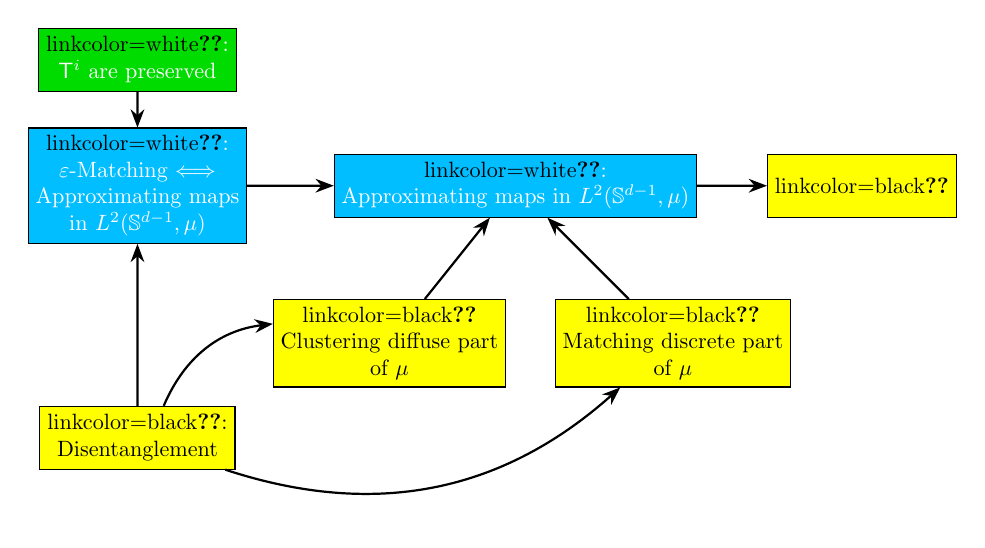
\begin{tikzpicture}[node distance=2cm, scale=0.8, every node/.style={transform shape}]

    % Define block styles
    \tikzset{
        section/.style={rectangle, minimum width=3cm, minimum height=1cm, text centered, draw=black, fill=#1},
        arrow/.style={thick, ->, >=Stealth}
    }

    % Nodes
    \node (1) [section=vibrantgreen, align=center] {
    {\hypersetup{linkcolor=white}\Cref{lem: hyp.propagation}{\color{white}:}}\\{\color{white}$\mathsf{T}^i$ are preserved}};
    \node (2) [section=skyblue, below of=1, align=center] {\hypersetup{linkcolor=white}\Cref{lem: monge}{\color{white}:}
    \\ {\color{white}$\varepsilon$-Matching $\Longleftrightarrow$}\\ {\color{white}Approximating maps}\\{\color{white}in $L^2(\S,\mu)$}};
    \node (3) [section=brightyellow, align=center, below of=2, yshift=-2cm] {\hypersetup{linkcolor=black}\Cref{prop: separation}:\\Disentanglement};
    \node (4) [section=skyblue, right of=2, xshift=4cm, align=center] {\hypersetup{linkcolor=white}\Cref{lem: univ.approx}\color{white}:\\ \color{white}Approximating maps in $L^2(\S,\mu)$};
    \node (5) [section=brightyellow, right of=4, xshift=3.5cm, align=center] {\hypersetup{linkcolor=black}\Cref{thm: main.result}};
    \node (6) [section=brightyellow, below of=2, xshift=4cm, yshift=-0.5cm, align=center] {\hypersetup{linkcolor=black}\Cref{prop: compression}\\ Clustering diffuse part\\ of $\mu$};
    \node (7) [section=brightyellow, below of=4, xshift=2.5cm, yshift=-0.5cm, align=center] {\hypersetup{linkcolor=black}\Cref{prop: interpolation.neural.ode}\\ Matching discrete part\\ of $\mu$};

    % Arrows
    \draw [arrow] (1) to (2);
    \draw [arrow] (2) -- (4);
    \draw [arrow] (4) -- (5);
    \draw [arrow] (3) -- (2);
    \draw [arrow] (6) -- (4);
    \draw [arrow] (7) -- (4);
    \draw [arrow, bend left] (3) to (6); % Curved arrow
    \draw [arrow, bend right] (3) to (7); % Curved arrow

    \end{tikzpicture}
    \caption{High-level overview of the proof of \Cref{thm: main.result}. %\ndpr{I can't read what's in the blue and green boxes when printing out. Please  use different colors like white text or lighter background colors.}\nbbg{bg: done}
    }
    \label{fig: overview.2}
\end{figure}

Matching general ensembles of measures \emph{cannot} be done with a single \emph{linear} continuity equation, as is done in the Benamou-Brenier reformulation of optimal transport for instance \cite{benamou2000computational}, namely \eqref{eq: cauchy.pb} in which the vector field $v$ does not depend on $\mu(t)$. Indeed, take for instance $\mu_0^1,\mu_0^2\in\mathscr{P}_{\mathrm{ac}}(\S)$ such that 
$$\supp(\mu_0^1)\cap \supp(\mu_0^2)\neq\varnothing,$$
and similarly $\mu_1^1,\mu_1^2\in \mathscr{P}_{\mathrm{ac}}(\S)$ such that
\begin{equation} \label{eq: empty.intersection}
\supp(\mu_1^1)\cap \supp(\mu_1^2)=\varnothing.
\end{equation}
Then there cannot exist a single-valued $\mathsf{T}:\S\to\S$ such that $\mathsf{T}_\#\mu_0^1=\mu_1^1$ and $\mathsf{T}_\#\mu_0^2=\mu_1^2$, since there would have to exist $x\in \supp(\mu_0^1)\cap \supp(\mu_0^2)$ for which $\mathsf{T}(x)$ would have to take two different values due to \eqref{eq: empty.intersection}. This elementary counterexample is the starting point of our strategy, as the self-attention mechanism $\mathscr{A}_{\bB}[\mu]$ provides a nonlinear dependence\footnote{One can draw parallels with the failure of the Kalman rank condition \cite{sontag2013mathematical, coron2007control} for the ensemble controllability of linear systems in finite dimensions.} of the solution map to \eqref{eq: cauchy.pb} with respect to $\mu$, which we use precisely to disentangle overlapping measures. In this regard, \Cref{thm: main.result} is an ensemble controllability result for a {\it nonlinear} continuity equation, thus extending existing results on the controllability of the {\it linear} continuity equation---see \cite{brockett2008control, khesin2009, agrachev2009controllability, agrachev2009optimal, raginsky2024some, chen2016optimal, duprez2019approximate}.

\subsection{Outline} The remainder of the paper is organized as follows. We comment on assumptions and extensions of \Cref{thm: main.result} in {\bf \Cref{sec: discussion}}. In {\bf \Cref{sec: clustering}}, we provide explicit parameters that yield long-time clustering (i.e., convergence to discrete measures). {\bf \Cref{sec: disentanglement}} presents how initial measures with overlapping support can be disentangled over time using clustering. {\bf \Cref{sec: neural.ode}} addresses the matching problem of clouds of points, which is used after clustering and disentanglement. The proofs of \Cref{thm: main.result} and \Cref{thm: targets.atoms} can be found in {\bf \Cref{sec: proofs}}. We discuss some interesting questions regarding the number of switches needed for disentanglement in {\bf \Cref{sec: complexity.untanglement}}.


\subsection{Discussion} \label{sec: discussion}

\subsubsection{On our assumptions}  

\begin{itemize}
    \item The requirement $d \geq 3$ in \Cref{thm: main.result} stems from matching disentangled measures. In $d = 2$, the problem becomes intrinsically one-dimensional, and in such a setting, the order of particles is preserved. This obstruction impedes the conclusion of the disentanglement. To carry through our strategy, one needs to use self-attention to order the input measures and disentangle them.


    \item When the targets are more general than point masses---as in \Cref{thm: main.result}---we operate under the assumption that there exists a transport map between every pair $(\mu_0^i, \mu_1^i)$. This is again satisfied for many cases of interest; for instance, whenever $\mu_0^i$ is absolutely continuous with respect to the Lebesgue measure on $\S$ (per the celebrated theorem(s) of Brenier-McCann \cite{brenier1991polar, mccann2001polar}), or whenever $\mu_0^i$ and $\mu_1^i$ are empirical measures with $\mu_0^i$ having as many atoms as $\mu_1^i$. This assumption is also minimal. Indeed, since $v[\mu(t)](t,\cdot)$ is Lipschitz, any solution to \eqref{eq: cauchy.pb} can be written as the image measure of the initial data by means of some map. This presents a natural impediment to matching a measure constituted by a single atom to a measure with two atoms.

    \item If the input $\mu_0^i$ and output $\mu_1^i$ are empirical measures having $n$ and $m$ atoms respectively, 
    with $n > m$ and $\frac{n}{m} \notin \mathbb{N}$, then there does not exist a transport map between $\mu_0^i$ and $\mu_1^ i$. 
    Consequently, for the same reason as in the previous point, it is not possible to find a solution to \eqref{eq: cauchy.pb} that approximates $\mu_1^i$ to any desired level of accuracy. However, if to each atom of $\mu_1^i$ one assigns  $\lfloor n/m \rfloor$ atoms of $\mu_0^i$, then one can construct a map $\mathsf{T}^i$ such that $\mathsf{W}_2(\mathsf{T}_\#^i\mu_0^i, \mu_1^i) = O\left(m/n\right)$. As a result, we could use the flow map of  \eqref{eq: cauchy.pb} to approximate all $N$ target measures 
     to error $O(\varepsilon+m/n)$.
\end{itemize} 

\subsubsection{On exact matching} 
One can raise the natural question if it is possible to have \emph{exact} matching. i.e. $\varepsilon=0$, in \Cref{thm: main.result}. We provide some comments:

\begin{itemize}
    \item We can exactly match $N$ empirical input measures to $N$ empirical target measures as long as they have the same number of atoms. This follows as a corollary of the proof of \Cref{thm: main.result}, since no quantization is required in \Cref{lem: univ.approx}. %\npdr{What if source has more atoms than target? I wrote this just before the beginning of 1.4.2 when you talk about Brenier but you seem to insist on the same support size so I'm not sure. Please check.} \nddrb{The second paragraph of 1.4.1 corrected and a third point added}
    
    \item Since $v[\mu(t)](t,\cdot)$ is Lipschitz, we cannot do exact transportation of an absolutely continuous measure to a discrete one even when $N=1$. Similarly, we cannot match a single input measure with connected support to a target measure whose support has multiple connected components. 
\end{itemize}

\begin{remark}[Beyond $\mathsf{W}_2$] We opted for approximation in the Wasserstein distance because working with distances is convenient. The result could be adapted to encompass the Kullback-Leibler divergence  $(\mathsf{KL})$, which is the natural candidate in view of applications.
%(Due to the compactness of $\S$,
(Note that this would be a stronger approximation result by virtue of \cite{bolley2005weighted}, which only requires the second argument in the $\mathsf{KL}$ to have a Gaussian moment, guaranteed in our case by working on $\S$.)
%Talagrand's $T_2$-inequality \cite{otto2000generalization}.)
%\ndpr{Talagrand's $T_2$ inequality does not hold for any measure so you cannot invoke it without further assumptions. You can use Bolley-Villani though. It only requires the second argument in the KL to have Gaussian moment.} \nddrb{Corrected}
To achieve this, after the step involving the disentanglement of supports, we can match the disentangled measures approximately in $\mathsf{TV}$ instead of $\mathsf{W}_2$ by following a similar approach to the one developed in \cite{ruiz2024control}, and then apply a reverse Pinsker inequality \cite[Theorem 7]{verdu2014total} (see also \cite{sason2016f}). However, to do so, one needs that the measures are mutually absolutely continuous and to have a bounded likelihood ratio. %\npdr{Do you really think this is something we can ever achieve?}%under the assumption that $\mu\ll\nu$ and $\nu\ll\mu$, and $\left\|\frac{\diff \mu}{\diff \nu}\right\|_{L^\infty(\S)}\geq 1 $ \cite[Theorem 7]{verdu2014total} asserts
%\begin{equation*}
%    \mathsf{KL}(\mu||\nu)\lesssim \left\|\frac{\diff \mu}{\diff \nu}\right\|_{L^\infty(\S)}^{\frac{1}{2}}|\mu-\nu|_{\mathsf{TV}(\S)}.
%\end{equation*}
%\ndpr{what's a reverse Pinsker inequality? Does it hold in general? I think you need to the measures to be very close in a strong sense for this to hold; e.g. bdd likelihood ratio} \nddrb{references and hypothesis added} 
This approach would avoid quantizing the (disentangled) target measure and thus clustering the (disentangled) inputs into atoms.
\end{remark}

\begin{comment}
\begin{remark}[Infinite-dimensional transport]
{\color{white}.}

\begin{enumerate}
    \item \Cref{thm: main.result} is an instance of approximation of regular maps from $\mathscr{P}(\S)$ to itself. Let $f:\mathscr{P}(\S)\to\mathscr{P}(\S)$ be 1-Lipschitz:
\begin{equation*}
    \mathsf{W}_2(f(\mu),f(\nu))\leq\mathsf{W}_2(\mu,\nu).
\end{equation*}
Fix $\pi\in\mathscr{P}(\mathscr{P}(\S))$ and $\varepsilon>0$. One then seeks to find $\theta^\varepsilon\in L^\infty((0,T);\Uptheta)$ such that the solution map $\Phi_{\theta^\varepsilon}^T:\mathscr{P}(\S)\to\mathscr{P}(\S)$ of \eqref{eq: cauchy.pb} satisfies
\begin{equation*}
    \int\mathsf{W}_2\left(\Phi_{\theta^\varepsilon}^T(\mu), f(\mu)\right)\pi(\mu)\leq\varepsilon.
\end{equation*}
\Cref{thm: main.result} provides a positive answer when $\pi$ is an empirical measure over probability measures on $\S$, but the question can be asked in full generality---this remains open. \ndpr{Okay, I guess you can ask this question, but I'm not sure anyone would care really.}

\item Another question\footnote{We thank Gabriel Peyré for raising this question and for discussions.} which our analysis could yield an answer to is the following. Suppose $f:\mathscr{P}(\S)\to\mathscr{P}(\S)$ preserves cardinality when acting on discrete measures. Can one then write $f(\mu)=(\mathsf{T}_\mu)_\#\mu$ for some $\mathscr{P}(\S)\ni\mu\mapsto\mathsf{T}_\mu\in L^2(\S;\S)$ which is continuous with respect to $\mu$ (in the sense of weak convergence)? A possible avenue for answering this question is to note that the characteristic flow of \eqref{eq: cauchy.pb} allows to write $\Phi_{\theta^\varepsilon}^T(\mu)=(\mathsf{T}_\mu^\varepsilon)_\#\mu$
for some $\mathsf{T}_\mu^\varepsilon\in L^2(\S;\S)$ which is continuous in $\mu$. An affirmative answer to the question would follow should one be able to pass to the limit as $\varepsilon\to0$, which, while not immediate from our results (since the norm of the parameters blows up), appears plausible. \npdr{This is not a very clean question. I have a vague sense of what you want to do her but why continuous and not Lipschitz? What's the point of finding this map?. I suggest removing it. Also removing the previous remark in fact. I don't want to be the guy asking question in my paper for profiling purposes: if a students comes to me and tells me they have solved this question, I will probably run away.} \nbbg{bg: fine for me, we can remove.}
\end{enumerate}
    

\end{remark}    
\end{comment}




\subsubsection{On the number of parameter switches} \label{sec: nb.disc}

Our proof roughly yields
\begin{equation*}
    \#\text{switches} =  \#\text{switches}_{\text{disentanglement}} + \#\text{switches}_{\text{clustering}} + \#\text{switches}_{\text{matching}}
\end{equation*}
for piecewise constant parameters. Our current best estimate, if all measures have pairwise overlapping support, is 
\begin{equation*}
 \#\text{switches}_{\text{disentanglement}} = O(d \cdot N).   
\end{equation*}
(See {\bf \Cref{sec: complexity.untanglement}} for an extended discussion thereon.)
While all the parameters involved in the construction of the final map $\Phi_{\text{fin}}^T$ yielding \Cref{thm: main.result} are explicit, the precise estimate of $\#\text{switches}$ in the most general case is difficult to determine, due to the clustering step. We discuss three concrete cases.


\begin{enumerate}
    \item In \Cref{thm: targets.atoms}, once the input measures are rendered disentangled, we use a single constant parameter that results in clustering over time (as per \cite{geshkovski2023mathematical}), collapsing each input measure to a point mass. Thus, 
    $$\#\text{switches}_{\text{clustering}}=0.$$
    The resulting ensemble of point masses can then be matched to the targets using the perceptron component (adapting ideas from \cite{ruiz2023neural, li2022deep}) with 
    $$\#\text{switches}_{\text{matching}}=O(N).$$
    So the switches in \Cref{thm: targets.atoms} arise primarily from the disentangling step. In particular, if the source measures have disjoint support, then the number of switches becomes $O(N)$ which is dimension independent.

    
    \item Consider \Cref{thm: main.result}, with targets that are empirical measures having $m \geq 2$ atoms, and inputs that are all absolutely continuous. As seen in \Cref{proof: proof.restricted} (restricted case), the proof can be significantly simplified in this case. Indeed, one can avoid a direct application of \Cref{lem: univ.approx} and \Cref{prop: compression} by instead iteratively applying \Cref{lem: two.balls}
    to each input measure. Namely, after the disentanglement step (with a sufficiently large separation), we partition the support of each disentangled input measure into $m$ pieces, which we can cluster to a point with a single constant parameter per piece using \Cref{lem: two.balls}. All in all, 
    $$\#\text{switches}_{\text{clustering}} = O(m\cdot N).$$
    The resulting clustered measures can then be matched to the empirical target measures by \Cref{prop: interpolation.neural.ode} at the cost of 
    $$\#\text{switches}_{\text{matching}} = O(m \cdot N).$$  
    All in all,
    $$
    \#\mathrm{switches} = O\big((m+d)N\big).
    $$
    
    \item Suppose both the inputs and targets are empirical measures, with $n$ and $m$ atoms, respectively. 
    When it comes to $\#\text{switches}_{\text{clustering}}$, if $n \gg m$ or $m$ is a divisor of $n$, one can use $m$ balls per measure in \Cref{prop: compression} instead of packing, which would lead to 
    $$\#\text{switches}_{\text{clustering}} = O(m \cdot N).$$ 
    To achieve this, one can combine \Cref{prop: separation} with the clustering of measures to a point mass as in \Cref{prop: targets.atoms}, much like what is done in the \Cref{proof: proof.restricted} (restricted case). 
    By virtue of the latter, we can partition the support of each measure using large balls that are not necessarily contained within the support. All in all,
    $$
    \#\mathrm{switches} = O\big((m+d)N\big).
    $$
    %\ndpr{need to compare this with existing results for sequence-to-sequence} \nbbg{done to the best of our ability}
    To put things into context: in the discrete-time setting of \cite{yun2019transformers}, while the number of layers is seemingly independent of the number of sequences $N$, it is exponential in the dimension $d$.
\end{enumerate}
In the case of general target measures as in \Cref{thm: main.result}, $\#\text{switches}_{\text{clustering}}$ is exponential in the dimension $d$ due to the use of a specific strategy which leverages packing numbers---see \Cref{rem: nb.disc.clustering}. 





\subsubsection{On generalities}
We comment on even greater generality in the choice of the Transformer architecture, which typically varies slightly from implementation to implementation. (See {\bf \Cref{app: code}} for further details.)

\begin{itemize}
    \item {\bf Increasing the width.} Many of the actions used throughout our proofs are performed using the perceptron component with constant parameter matrices $\bW$ and $\bU$ that are of rank 1. One could, of course, consider using rectangular matrices instead, thus increasing the \emph{width} of the network, which could, in turn, reduce the number of switches ($\approx$ depth).
    
    \item {\bf Multi-head attention.} The computation of token similarities through self-attention is typically parallelized in practice throughout several \emph{heads}, lending way to \emph{multi-head self-attention}. This boils down to replacing the term 
    $$\bV(t)\mathscr{A}_{\bB}[\mu(t)](t,x)$$ 
    in \eqref{eq: vf} by
    \begin{equation*}
        \sum_{h=1}^H \bV_h(t)\mathscr{A}_{\bB_h}[\mu(t)](t,x).
    \end{equation*}
    We now dispose of $H\geq1$ parameters $(\bV_h(t),\bB_h(t))_{h\in[H]}$ at every time $t$. We do not know how to exploit multiple heads in our proofs, although some theoretical insights thereon can be found in the proofs in \cite{chen2024provably}.

    \item  {\bf Discrete time.} The continuous-time formulation gives rise to an equation that is \emph{reversible in time}, which we often use in our construction. In particular, the task of disentangling supports becomes equivalent to the task of entangling supports, which is not the case in the non-reversible scenario. Our results are expected to hold for an appropriate discretization of \eqref{eq: cauchy.pb} with a sufficiently small time step.

    \item {\bf Beyond the ReLU perceptron.} All of our results remain unchanged if one replaces $(\cdot)_+$ (the ReLU) by any other Lipschitz nonlinearity that equals the ReLU near the origin. It is likely that the proofs can be generalized to even encompass the hyperbolic tangent. The relevant property that the nonlinear activation function ought to satisfy is to ensure that the resulting  flow (when $\bV\equiv0$) leaves any spherical cap of choice invariant. 
\end{itemize}


\subsection{Notation and basic definitions} 
Unless stated otherwise, all integrals are taken over $\S$, and all $\nabla$ denote the spherical gradient. We use $[n]:=\{1,\ldots,n\}$, and $f(x) \lesssim g(x)$ if there exists a finite positive constant $C$ such that $f(x) \leq Cg(x)$. We write $f(x) \lesssim_S g(x)$ if the resulting constant depends on $S$. We denote by $d_g(x,y)$ the geodesic distance between $x, y \in \S$, which, as a reminder, is the great-circle distance $d_g(x,y) = \arccos(\langle x, y \rangle)$. For $A \subset \S$, we denote by $\mathrm{conv}\, A$ the convex hull of $A$ in $\mathbb{R}^d$, and by $\conv_g\, A$ the geodesic convex hull of $A$ in $\S$ (the smallest geodesically convex set containing $A$). Unless otherwise specified, all open balls are considered as subsets of $\S$ and are taken with respect to $d_g$. 
%\npdr{I don't understand what "with the norm ..." means here} \nbbg{bg: old remnant, removed.} 
Recall the Wasserstein-$p$ distance for $p\geq 1$:
\begin{equation} \label{eq: wass.dist}
    \mathsf{W}_p^p(\mu,\nu):=\inf_{\pi\in \mathcal{C}(\mu,\nu)}\int d_g(x,y)^p\pi(\diff x,\diff y),
\end{equation}
where $\mathcal{C}(\mu,\nu)$ denotes all couplings between $\mu$ and $\nu$ (see \cite{villani2009optimal} for details). 
We set \( \mathsf{W}_\infty(\mu,\nu) := \lim_{p \to +\infty} \mathsf{W}_p(\mu,\nu) \). A geodesic is a smooth curve with zero acceleration, namely, a smooth \( \gamma: I \to \S \) with \( \proj_{\gamma(t)}(\ddot{\gamma}(t)) = 0 \) for \( t \in I \), where \( I \) is an open interval. Geodesics on \( \S \) lie on great circles, specifically, there exists \( v \in \S \) such that
\[
\gamma(t) \subset \{x \in \S : \langle x, v \rangle = 0 \}\,, \quad \forall\, t \in I\,.
\]
Given two points \( x, y \in \S \), a geodesic \( \gamma: [a,b] \to \S \) is called a minimal or minimizing geodesic between \( x \) and \( y \) if \( \gamma \) is of speed 1 (i.e., \( \|\dot{\gamma}(t)\| = 1 \)), satisfies \( \gamma(a) = x \) and \( \gamma(b) = y \), and \( d_g(x,y) = b - a \). If \( x \) and \( y \) are not antipodal, the minimizing geodesic between them is unique and is simply the segment between them on the great circle on which they both lie. The geodesic open ball of radius $R>0$ centered at $x\in\S$ is defined as
\begin{equation} \label{eq: geodesic.ball.def}
    B(x,R)\coloneqq\left\{y\in \S:\, d_g(x,y)< R \right\}.
\end{equation}
Unless stated otherwise, by open (resp. closed) ball we understand a \emph{geodesic} open (resp. closed) ball.

\subsubsection*{Acknowledgments} 

B.G. acknowledges financial support from the French government managed by the National Agency for Research under the France 2030 program, with the reference ”ANR-23-PEIA-0004”.
P.R. was supported by NSF grants DMS-2022448, CCF-2106377, and a gift from Apple.
D. Ruiz-Balet was funded by the UK Engineering and Physical Sciences Research Council (EPSRC) grant
EP/T024429/1.


\section{Clustering of the input data} \label{sec: clustering}

We begin by investigating how the input measures can be clustered using \eqref{eq: cauchy.pb}, in the sense that they are in the vicinity of discrete measures with few atoms.

In {\bf \Cref{sec: diracs}}, we cover the special case of clustering to a single atom, while the case of general discrete measures is discussed in {\bf \Cref{sec: general.dirac}}. The results of this section are used in {\bf \Cref{sec: disentanglement}}, and they are also a key step in our final matching strategy.

\subsection{Clustering to a single point mass} \label{sec: diracs}

The following is essentially an adaptation of the so-called ``cone collapse'' argument presented in \cite[Lemma 6.4]{geshkovski2023mathematical}.

\begin{proposition} \label{prop: targets.atoms}
Suppose $\mu_0^i\in \mathscr{P}(\S)$ for $i\in[N]$, are such that 
\begin{equation*}
\supp(\mu_0^i)\text{ is contained in an open hemisphere.}
\end{equation*} 
Fix $\bB\in \mathscr{M}_{d\times d}(\mathbb{R})$. Then, for any $i\in[N]$, there exists $z^i\in \conv_g\,\supp(\mu_0^i)$ such that the following holds. For any $\varepsilon>0$, there exists $T>0$ such that, the unique solution $\mu^i$ to
\begin{equation} \label{eq: cauchy.pb.W=0}
\begin{cases}
\partial_t \mu^i(t)+\dive\left(\proj_x\mathscr{A}_{\bB}[\mu^i(t)]\mu^i(t)\right)=0 &\text{ on } [0,T]\times\S\\
\mu^i(0)=\mu_0^i &\text{ on } \S   
\end{cases}
\end{equation}
satisfies
\begin{equation*}
\mathsf{W}_{\infty}\left(\mu^i(T),\updelta_{z^i}\right)\leq \varepsilon.
\end{equation*}
%for some $z^i\in\conv_g(\supp(\mu_0^i))$. 
Moreover if
\begin{equation*}
\supp(\mu_0^i)\cap \supp(\mu_0^j)=\varnothing
\end{equation*}
for all $i\neq j\in[N]$ then $z^i\neq z^j$ for all $i\neq j\in[N]$.
\end{proposition}


\begin{proof}[Proof of \Cref{prop: targets.atoms}] 
It suffices to show the result for a single measure. We therefore drop indices to lighten the notation.
Suppose\footnote{$\upsigma_d$ henceforth denotes the normalized spherical Lebesgue measure, i.e. the uniform measure.}
\begin{equation*}
    \upsigma_d(\conv_g\,\supp(\mu_0))>0.
\end{equation*}
Since $\bV=I_d$, and $\supp(\mu_0)$ being contained in a half-sphere, for all 
$x\in \supp(\mu_0)$ we have
\begin{equation}\label{eq: attention.b.1}
    \|\mathscr{A}_{\bB}[\mu_0](x)\|>0,
\end{equation}
and
\begin{equation}\label{eq: attention.b.2}
    \gamma(x):=\frac{\mathscr{A}_{\bB}[\mu_0](x)}{\|\mathscr{A}_{\bB}[\mu_0](x)\|}\in \mathrm{int}\left(\conv_g\,\supp(\mu_0)\right).
\end{equation}
Now fix $\tau>0$ and $x_0\in\partial \conv_g\,\supp(\mu_0)$, and consider $x$ solving
\begin{equation}\label{eq: char.flow}
    \begin{cases}
        \dot{x}(t)=\proj_{x(t)}\left(\mathscr{A}_{\bB}[\mu(t)](x(t))\right)\quad t\in [0,\tau]\\
        x(0)=x_0.
    \end{cases}
\end{equation}
We Taylor expand: 
\begin{align*}
    \left\langle x(\tau), \gamma(x_0) \right\rangle = \left\langle x_0, \gamma(x_0) \right\rangle+ \tau\left\langle \proj_{x_0}(\mathscr{A}_{\bB}[\mu_0](x_0)), \gamma(x_0) \right\rangle+O(\tau^2).
\end{align*}
Using $\mathscr{A}_{\bB}[\mu_0](x_0)=\proj_{x_0}(\mathscr{A}_{\bB}[\mu_0](x_0))+ \left\langle \mathscr{A}_{\bB}[\mu_0](x_0),x_0 \right\rangle x_0 $ as well as \eqref{eq: attention.b.1}, we deduce
\begin{equation*}
   \tau\left\langle \proj_{x_0}(\mathscr{A}_{\bB}[\mu_0](x_0)), \gamma(x_0)\right\rangle=\tau  \frac{\|\proj_{x_0}(\mathscr{A}_{\bB}[\mu_0](x_0))\|}{\|\mathscr{A}_{\bB}[\mu_0](x_0)\|} >0.
\end{equation*}
Therefore $\left\langle x(\tau), \gamma(x_0) \right\rangle> \left\langle x_0, \gamma(x_0) \right\rangle$ for $\tau$ small enough. In view of \eqref{eq: attention.b.2}, we deduce
\begin{equation*}
    x(\tau)\in \mathrm{int}(\conv_g\,\supp(\mu_0)).
\end{equation*}
This entails that $t\mapsto \conv_g\,\supp(\mu(t))$ is strictly non-increasing (in the sense of set inclusion) for short times, i.e.
\begin{equation}\label{eq: set.inclusion}
        \conv_g\,\supp(\mu(\tau))\subset \conv_g\,\supp(\mu_0)
\end{equation}
for $\tau$ small enough. By the Lipschitz character of \eqref{eq: char.flow}, we also gather that 
$$\upsigma_d(\conv_g\,\supp(\mu(t)))>0$$
for all finite $t\geq 0$.
Therefore we can bootstrap the argument for obtaining \eqref{eq: set.inclusion} to deduce that $t\mapsto \conv_g\,\supp(\mu(t))$ is strictly non-increasing over $\mathbb{R}_{\geq 0}$, and we also see that 
\begin{equation}\label{eq: lebesgue.going.zero}
\lim_{t\to+\infty}\upsigma_d(\conv_g\,\supp(\mu(t)))=0. 
\end{equation}
We use \eqref{eq: lebesgue.going.zero} and induction over the dimension $d$ to conclude. Indeed note that in $d=2$, \eqref{eq: lebesgue.going.zero} and the Portmanteau theorem yield
\begin{equation} \label{eq: d=1.case}
    \lim_{t\to +\infty}\mathsf{W}_\infty(\mu(t),\delta_{x^*})=0
\end{equation}
for some $x^*\in \mathbb{S}^1$ depending only on $\mu_0$. 
Now suppose $d=3$. By \eqref{eq: lebesgue.going.zero} and the Portmanteau theorem, for every $\varepsilon_1>0$ there exist $T_{\varepsilon_1}>0$ and $\mu_{\varepsilon_1}^0\in \mathscr{P}(\mathbb{S}^{d-1})$ such that $   \supp(\mu_{\varepsilon_1}^0)\subset \mathbb{S}^1\cap \{x\colon x_2>0\}$ and
\begin{equation} \label{eq: first.winfty}
\mathsf{W}_{\infty}\left(\mu(T_{\varepsilon_1}),\mu_{\varepsilon_1}^0\right)\leq \varepsilon_1.
\end{equation}
By virtue of \eqref{eq: d=1.case}, for every $\varepsilon_2>0$ there exist $T_{\varepsilon_2}>0$ and $x^*_{\varepsilon_1}$ (depending on $\varepsilon_1$ through the initial measure $\mu_{\varepsilon_1}$) such that the solution $\mu_{\varepsilon_1}$ to
\begin{equation*}
\begin{cases}
\partial_t\mu_{\varepsilon_1}+\dive\left(\proj_x\mathscr{A}_{\bB}[\mu_{\varepsilon_1}(t)]\mu_{\varepsilon_1}\right)=0 &\text{ on } [T_{\varepsilon_1},T_{\varepsilon_1}+T_{\varepsilon_2}]\times \mathbb{S}^{d-1}\\
    \mu_{\varepsilon_1}(T_{\varepsilon_1})=\mu_{\varepsilon_1}^0 &\text{ on } \S
\end{cases}
\end{equation*}
satisfies
\begin{equation} \label{eq: second.winfty}
\mathsf{W}_{\infty}\left(\mu_{\varepsilon_1}(T_{\varepsilon_2}+T_{\varepsilon_1}),\delta_{x^*_{\varepsilon_1}}\right)\leq \varepsilon_2.
\end{equation}
Combining \eqref{eq: first.winfty}, \eqref{eq: second.winfty} with the triangle inequality and \Cref{lem: gronwall.transfer.plan}, we have
\begin{align*}
\mathsf{W}_\infty\left(\mu(T_{\varepsilon_2}+T_{\varepsilon_1}),\delta_{x^*_{\varepsilon_1}}\right)
&\leq \mathsf{W}_\infty\left(\mu(T_{\varepsilon_2}+T_{\varepsilon_1}),\mu_{\varepsilon_1}(T_{\varepsilon_2}+T_{\varepsilon_1})\right)\\
&\hspace{1cm}+\mathsf{W}_\infty\left(\mu_{\varepsilon_1}(T_{\varepsilon_2}+T_{\varepsilon_1}),\delta_{x^*_{\varepsilon_1}}\right)\\
&\leq O\left(e^{e^{T_{\varepsilon_2}}}\right)\mathsf{W}_\infty\left(\mu(T_{\varepsilon_1}),\mu_{\varepsilon_1}\right)+\varepsilon_2\\
    &\leq O\left(e^{e^{T_{\varepsilon_2}}}\right)\varepsilon_1+\varepsilon_2,
\end{align*}
where the implicit constants are independent of $\varepsilon_1,\varepsilon_2$.
By compactness, there exists $x^*\in\mathbb{S}^1$ such that for any sequence $\varepsilon_{1,n}\to 0$ as $n\to +\infty$, there is a subsequence $\{\varepsilon_{1,n_k}\}_{k\in \mathbb{N}}$ such that $x_{\varepsilon_{1,n_k}}\to x^*$ as $k\to+\infty$. 
We relabel this subsequence as $\varepsilon_{1,n}$ and the associated sequence of times by $\{T_{\varepsilon_{1,n}}\}_{n\in\mathbb{N}}$. 
Now note that
\begin{align}
    \mathsf{W}_{\infty}\left(\mu(T_{\varepsilon_{2}}+T_{\varepsilon_{1,n}}),\delta_{x^*}\right)&\leq O\left(e^{e^{T_{\varepsilon_2}}}\right)\varepsilon_{1,n}+\varepsilon_2+d_g\left(x_{\varepsilon_{1,n}}^*,x^*\right). \label{eq: triangle}
\end{align}
Moreover, there exists some $n(\varepsilon)\geq 1$ such that 
\begin{equation*}
    d_g\left(x_{\varepsilon_{1,n}}^*,x^*\right)\leq \frac{\varepsilon}{3}
\end{equation*}
for all $n\geq n(\varepsilon)$.
We set $\varepsilon_2=\frac{\varepsilon}{3}$ and we choose $n\geq n(\varepsilon)$ large enough so that
\begin{equation*}
    O\left(e^{e^{T_{\varepsilon_2}}}\right)\varepsilon_{1,n}\leq \frac{\varepsilon}{3}.
\end{equation*}
Coming back to \eqref{eq: triangle}, we find 
\begin{equation*}
    \mathsf{W}_{\infty}\left(\mu\left(T_{\varepsilon_{1,n}}+T_{\frac{\varepsilon}{3}}\right),\delta_{x^*}\right)\leq \varepsilon
\end{equation*}
%where $T_{\frac{\varepsilon}{3}}>T_{\varepsilon_{1,n}}$
for $n\geq n(\varepsilon)$. Therefore, we found a sequence of positive times $\{T_n\}_{n\in \mathbb{N}}$ with $T_n=T_{\varepsilon_{1,n}}+T_{\frac{\varepsilon}{3}}$ for which $\mu_n=\mu(T_n)$ converges to $\delta_{x^*}$ in $\mathsf{W}_\infty$. Thanks to  \eqref{eq: set.inclusion}, the convergence does not depend on the sequence of times. Indeed, for every $t\geq T_n$, we have
\begin{align*}
    \mathsf{W}_\infty(\mu(t),\delta_{x^*})\leq\max_{y\in \mathrm{conv}_g\supp(\mu(t))}d_g(y,x^*)&\leq \max_{y\in \mathrm{conv}_g\supp(\mu_n)}d_g(y,x^*)\\
    &\leq\max_{y\in B(x^*,\mathsf{W}_\infty(\mu_n,\delta_{x^*}))}d_g(y,x^*)\\
    &=2\mathsf{W}_\infty(\mu_n,\delta_{x^*})\\
    &\leq 2\varepsilon
\end{align*}
where $B_n\coloneqq B(x^*,\mathsf{W}_\infty(\mu_n,\delta_{x^*}))$ is the ball on $\S$ centered at $x^*$ with radius $\mathsf{W}_\infty(\mu_n,\delta_{x^*})$. As $B_n$ is geodesically convex, and since $\supp(\mu_n)\subset B_n$, one has  $\mathrm{conv}_g\supp(\mu_n)\subset B_n$.

The cases $d>3$ follow by repeating the above argument.
\end{proof}

We can in fact even show the following quantitative estimate.

\begin{proposition} \label{cl: cluster.rate}
Consider the setting of \Cref{prop: targets.atoms}, for a fixed index $i$ (which we remove), and $\bB\equiv0$. Let $x_0\in\conv_g\,\supp(\mu_0)$ be the limit of $\mu(t)$.
Let $\varepsilon>0$ and set 
\begin{equation*}
T_\varepsilon:=%\inf_{\mathsf{W}_2(\mu(t),\updelta_{x_0})\leq \delta, x_0\in \S} t. 
\inf \left\{t\geq 0\colon \mathsf{W}_2(\mu(t),\updelta_{x_0})\leq \varepsilon\right\}.
\end{equation*}
Then 
\begin{equation*} 
T_\varepsilon=O\left(\log\frac{1}{\varepsilon}\right).
\end{equation*}
\end{proposition}

The proof can be found in {\bf \Cref{app: proof.cluster.time}}.




\subsection{Clustering to discrete measures} \label{sec: general.dirac}

The following result ensures that an ensemble of measures with disjoint supports can be clustered, up to arbitrary precision, to finitely many atoms within their own support, all by means of the same flow map. 

\begin{proposition} \label{prop: compression}
Suppose $\mu_0^i\in\mathscr{P}(\S)$, $i\in[N]$, have no atoms, and satisfy
\begin{equation*}
\conv_g\,\supp(\mu^i_0)\cap\conv_g\,\supp(\mu_0^j)=\varnothing
\end{equation*}
for $i\neq j$. Fix $M\geq1$, and for any $i\in[N]$ consider
\begin{equation*}
    \mu^i_1:=\sum_{k=1}^M \alpha_k^i \updelta_{x_{k}^i}
\end{equation*}
where $x_k^i\in\conv_g\,\supp(\mu_0^i)$, with $x_k^i = x_{k'}^j$ if and only if $(k, i) = (k', j)$, and where $\alpha_k^i\geq 0$ with $\sum_{k=1}^M\alpha_k^i=1$. Then for any $T>0$ and $\varepsilon>0$ there exist piecewise constant $(\bW,\bV,b):[0,T]\to\mathscr{M}_{d\times d}(\R)^2\times\R^d)$ such that for $i\in[N]$, the corresponding unique solution $\mu^i\in \mathscr{C}^0([0,T];\mathscr{P}(\S))$ to \eqref{eq: neural.pde.sphere} with data $\mu_0^i$ and these parameters satisfies
\begin{equation*}
\conv_g\,\supp\left(\mu^i(T)\right)\cap\conv_g\,\supp\left(\mu^j(T)\right)=\varnothing
\end{equation*}
for $i\neq j$, and 
\begin{equation*}
\mathsf{W}_2\left(\mu^i(T),\mu_1^{i}\right)\leq\varepsilon.
\end{equation*}
\end{proposition}

The number of switches in $(\bW,\bV, b)$ can also be accounted for---see \Cref{rem: nb.disc.clustering}.

%The proof of \Cref{prop: compression} makes use of the following.
%\ndpr{why is the next lemma in the main body and not the appendix?}




%We postpone the proof of \Cref{lem: tubular.mass.movement}
%to {\bf \Cref{proof: tubular.mass.movement}}, and proceed with that of \Cref{prop: compression}.

\begin{proof}[Proof of \Cref{prop: compression}]  We split
\begin{equation*}
    [0,T]=\bigcup_{i\in[N]} [T_{i-1},T_{i}],
\end{equation*}
where $0=T_0<T_1<\ldots<T_N=T$ are to be determined later on. 
We look to apply \Cref{lem: tubular.mass.movement} separately within each interval, thus, dealing with one measure at a time. Namely, the parameters take the form
\begin{equation*}
    (\bW,\bU,b)(t)=\sum_{i=1}^N (\bW_i,\bU_i,b_i)(t)1_{[T_{i-1},T_i)}(t),
\end{equation*}
where $(\bW_i,\bU_i,b_i)$ are, roughly speaking, piecewise constant parameters stemming from a repeated application of \Cref{lem: tubular.mass.movement}. We critically use \eqref{eq: eq.tubular.mass.movement} to ensure that when we act on the $i$-th measure in $[T_{i-1}, T_i]$, all the other measures remain invariant, so 
\begin{equation} \label{eq: init.invariant}
 \mu^i(T_{i-1}) = \mu_0^i.   
\end{equation}
Therefore, we take $i\in[N]$ to be arbitrary. We proceed in three steps.

\subsubsection*{Step 1. Partitioning each support into $M$ pieces}

Let $\mathscr{C}^i:=\supp(\mu^i_0)$, and consider a partition $\{\mathscr{C}^i_k\}_{k\in[M]}$ of $\mathscr{C}^i$ consisting of pairwise disjoint sets with connected interiors and satisfying
\begin{equation*}
    \mu_0^i(\mathscr{C}_k^i):=\alpha_k^i.
\end{equation*}
Namely
\begin{equation*}
\mathscr{C}^i=\bigcup_{k\in[M]} \mathscr{C}^i_k
\end{equation*}
with $\mathscr{C}_k^i\cap \mathscr{C}_{k'}^i=\varnothing$ if $k\neq k'$ (see \Cref{fig: shattering}).

\begin{figure}[!ht]
    \centering
    \includegraphics[scale=0.6]{figures/figure-2.pdf}
    \caption{Partitioning $\mathscr{C}^i:=\supp(\mu^i_0)$ into $M$ pieces with connected interiors.}
    \label{fig: shattering}
\end{figure}

\subsubsection*{Step 2. Packing each part $\mathscr{C}_k^i$ with balls}

We henceforth fix an arbitrary $i\in[N]$ and $k\in[M]$.
Let $\delta>0$ to be fixed and determined later on. Consider a packing of $\mathscr{C}_k^i$ consisting of $\mathsf{N}_{k}^i(\delta)\geq1$ disjoint open balls\footnote{Recall that all balls are considered as subsets of the sphere, so taken with respect to the geodesic distance, as in \eqref{eq: geodesic.ball.def}.} %\ndpr{Where do we define balls. These are on the sphere right? Since it's not that common and the picture is cartoony, I recommend (i) properly defining them and if it's done earlier in the paper but I didn't find it, (ii) recall what they are here}\nddrb{In the notation section, the definition is added and recalled in a footnote}
\begin{equation*}
B(z_{n,i,k},R_{n,i,k})\subset\mathscr{C}_k^i\hspace{1cm}\text{ for } n\in[\mathsf{N}_{k}^i(\delta)],
\end{equation*}
with $z_{n,i,k}\in \S$ and $R_{n,i,k}>0$, such that
\begin{equation}\label{eq: reminder.packing}
    \mu_0^i\left(\bigcup_{n\in[\mathsf{N}_{k}^i(\delta)]} B(z_{n,i,k},R_{n,i,k})\right)=\alpha_k^i-\delta.
\end{equation}
%\ndpr{You are doing two different things with zero explanation here.}
We now define a target ball contained in $\mathscr{C}_k^i$ to which we aim to send the mass contained in the packing \eqref{eq: reminder.packing}.
Fix the anchor point $x_{k}^i\in \mathrm{int}\left(\mathscr{C}^i_k\right)$, and let $\eta>0$ be arbitrary and to be determined later on (the same for all indices $(i, k)\in[N]\times[M]$), but also small enough so that
\begin{equation*}
\mathscr{B}_k^i:=B(x_{k}^i,\eta)\subset\mathrm{int}\left(\mathscr{C}^i_k\right).
\end{equation*}
We also choose the target ball $\mathscr{B}_k^i$ to satisfy $\mathscr{B}_k^i\subset B(z_{n,i,k},R_{n,i,k})$ for some $n\in[\mathsf{N}_k^i(\delta)]$ (see \Cref{fig: packing}).


\subsubsection*{Step 3. Sending most of the mass to $\mathscr{B}_k^i$}

\begin{figure}[!ht]
    \centering
    \includegraphics[scale=0.55]{figures/figure-3.pdf}
    \caption{ Step 2: packing the piece $\mathscr{C}_k^i$ of the partition of $\mathscr{C}^i=\mathrm{supp}(\mu_0^i)$ with balls whose union has mass $\mu_0^i(\mathscr{C}_k^i)-\delta$. A single anchor%\ndpr{Reference the word "anchor" in main text"} \nddrb{Done!  right below \eqref{eq: reminder.packing}} 
    point $x_k^i$ lies in this piece. The goal of Step 3 is to repeatedly use \Cref{lem: tubular.mass.movement} to transfer the mass of each ball to the one highlighted in blue. }
    \label{fig: packing}
\end{figure}


As $\mathrm{int}\left(\mathscr{C}^i_k\right)$ is connected and thus path-connected (both are equivalent for open sets in our setup), for every $n\in[\mathsf{N}_{k}^i(\delta)]$ we can find a sequence of open balls $\{\mathscr{B}_{\ell,n}\}_{0\leq\ell\leq L_{k, n}^i}\subset \mathscr{C}_k^i$ satisfying
\begin{equation}\label{eq: homotopy}
    \begin{aligned}
        &\mathscr{B}_{0,n}=B(z_{n,i,k},R_{n,i,k}),\\ 
        &\mathscr{B}_{\ell,n}\cap \mathscr{B}_{\ell+1,n}\neq \varnothing,\\
        &\mathscr{B}_{L_{n},n}=\mathscr{B}_k^i,\\
        &\mathscr{B}_{\ell,n}\cap\mathscr{B}_{\ell',n}=\varnothing\hspace{0.5cm}\text{ if }|\ell'-\ell|\geq 2.
    \end{aligned}
\end{equation}
Set $L_k^i:=\max_{n\in[\mathsf{N}_{k}^i(\delta)]} L_{n}$ and  fix an arbitrary $\overline{\varepsilon}>0$ to be determined later on. 
We apply \Cref{lem: tubular.mass.movement} for each piece $k\in[M]$ and $n\in[\mathsf{N}_k^i(\delta)]$---recalling \eqref{eq: init.invariant}---to find piecewise constant $(\bW_i, \bU_i, b_i):[T_{i-1}, T_i]\to\mathscr{M}_{d\times d}(\mathbb{R})^2\times\R^d$ with at most
\begin{equation*}
    K\cdot \max_{k\in[M]} \mathsf{N}_k^i(\delta)\cdot L_k^i
\end{equation*}
switches, such that
\begin{align}\label{eq: mass.lower.bound}
    \mu^i(T_i,\mathscr{B}_k^i)&\geq (1-\overline{\varepsilon})^{L_k^i} \mu_0^i\left(\bigcup_{n\in[\mathsf{N}_{k}^i(\delta)]}\bigcup_{\ell=0}^{L_{n}} \mathscr{B}_{\ell, n} \right)\nonumber\\
    &\geq (1-\overline{\varepsilon})^{L_k^i} \mu_0^i\left(\bigcup_{n\in[\mathsf{N}_{k}^i(\delta)]} B(z_{n,i,k},R_{n,i,k})\right)\nonumber\\
    &\overset{\eqref{eq: reminder.packing}}{=}(1-\overline{\varepsilon})^{L_k^i} \left(\alpha_k^i-\delta \right).
\end{align}
Moreover, $\mu^i(T_i)=\Phi^{T_i}_\#\mu^i_0$, and $\Phi^{T_i}(x)=x$ for all $x\notin \supp(\mu_0^i)$ because of \eqref{eq: eq.tubular.mass.movement}. 
Using Kantorovich-Rubinstein duality,
\begin{align*}
&\hspace{0.1cm}\mathsf{W}_1(\mu^i(T_i),\mu^i_1) = \sup_{\mathrm{Lip}(\phi)\leq 1}\left|\int\phi(\mu^i(T_i)-\mu_1^i)\right|\\
    &\hspace{0.2cm}= \sup_{\mathrm{Lip}(\phi)\leq 1}\left|\sum_{k=1}^M\int_{\mathscr{B}_k^i}\phi(\mu^i(T_i)- \mu_1^i)+\int_{\S\setminus(\bigcup_{k\in[M]}\mathscr{B}_k^i)}\phi(\mu^i(T_i)-\mu_1^i)\right|.
\end{align*}
Note that without loss of generality we can maximize over all $\phi\in W^{1,\infty}(\S)$ with $\mathrm{Lip}(\phi)\leq1$ and of average $0$. Such functions have an $L^\infty(\S)$--norm bounded by the length of any geodesic, namely $2\pi$.\footnote{We can write $\phi=\psi+\int\phi$ (vertical shift), and clearly $\|\psi\|_{\mathrm{Lip}(\S)}\leq1$. Since $\psi$ has average $0$ and is continuous, $\psi(x)=0$ for some $x\in\S$. Whence $|\psi(x)|\leq d_g(x,0)$ for $x\in\S$.} 
Going term by term in the identity above, using \eqref{eq: mass.lower.bound} and the definition of $\mathscr{B}_k^i$ we find
\begin{align*}
\int_{\mathscr{B}_k^i} \phi(\mu^i(T_i) -\mu_1^i)&=
    \int_{\mathscr{B}_k^i} \phi\mu^i(T_i) -\alpha_k^i\phi(x_k^i)\\
    &=\int_{\mathscr{B}_k^i} \phi\mu^i(T_i) -(\alpha_k^i-\overline{\delta})\phi(x_k^i)-\overline{\delta}\phi(x_k^i)\\
    &=\int_{\mathscr{B}_k^i} (\phi(x)-\phi(x_k^i))\mu^i(T_i) -\overline{\delta}\phi(x_k^i),
\end{align*}
where $\overline{\delta}:=\alpha_k^i-\mu^i(T_i,\mathscr{B}_k^i)>0$. 
By virtue of \eqref{eq: homotopy} and \eqref{eq: eq.tubular.mass.movement} we also gather that $\mu(T_i,\mathscr{C}_k^i)=\mu_0(\mathscr{C}_k^i)=\alpha_k^i$, and therefore 
$$\alpha_k^i=\mu^i(T_i,\mathscr{C}_k^i)\geq \mu^i(T_i,\mathscr{B}_k^i).$$
Owing to \eqref{eq: mass.lower.bound}, we find
\begin{equation*}
    \overline{\delta}\leq \alpha_k^i-(1-\overline{\varepsilon})^{L_k^i}(\alpha_k-\delta),
\end{equation*}
which clearly goes to $0$ as $\overline{\varepsilon}$ and $\delta$ go to $0$. Therefore
\begin{equation*}
    \left|\int_{\mathscr{B}_k^i} \phi(\mu^i(T_i) -\mu_1^i)\right|\leq \eta \mu^i(T_i,\mathscr{B}_k^i)+\overline{\delta}\|\phi\|_{L^\infty(\S)},
\end{equation*}
which tends to $0$ as $\delta$, $\overline{\varepsilon}$ and $\eta$ tend to zero. On the other hand, thanks to \eqref{eq: mass.lower.bound},
\begin{align*}
\left|\int_{\S\setminus(\bigcup_{k\in[M]}\mathscr{B}_k^i)}\phi(\mu^i(T_i)-\mu_1^i)\right|&\leq 2\pi \mu^i\left(T_i,\S\setminus\bigcup_{k\in[M]} \mathscr{B}_k^i\right)\\
    &\leq 2\pi \left|1-(1-\overline{\varepsilon})^{\max_{k\in[M]} L_k^i}\sum_{k=1}^M(\alpha_k^i-\delta)\right|\\
    &\leq 2\pi \left|1-(1-\overline{\varepsilon})^{\max_{k\in[M]} L_k^i}(1-M\delta)\right|,
\end{align*}
which also tends to 0 as $\overline{\varepsilon}$ and $\delta$ tend to $0$.
Therefore, we can choose $\overline{\varepsilon},\delta$ and $\eta$ small enough so that
\begin{equation*}
    \mathsf{W}_1\left(\mu^i(T_i),\mu_1^i\right)\leq \varepsilon.
\end{equation*}
We can conclude since all Wasserstein distances are equivalent on $\S$.
\end{proof}

\begin{remark} \label{rem: nb.disc.clustering}
    Looking at the proof, we deduce that $(\bW, \bU, b)$ have at most
    \begin{equation*}
    N \cdot M \cdot \max_{\substack{(i, k)\in[N]\times[M]}} \mathsf{N}_k^i(\delta) \cdot \max_{n\in[\mathsf{N}_k^i(\delta)]} L_{k,n}^i 
    \end{equation*}
    switches, where $\mathsf{N}_k^i(\delta)$ and $L_{k, n}^i$ are defined in Step 2 and Step 3 respectively.
    %\ndpr{How is this not exponential in the dimension??} \nbbg{it is exponential in the dimension, which is why this argument should be avoided (by having discrete targets for instance).}\ndpr{then we should have a remark to that effect when discussing the number of switches}

\end{remark}


\section{Disentangling supports} \label{sec: disentanglement}

In this section we show that flows generated by Transformers can disentangle measures with overlapping supports, in the sense that if
\begin{equation*}
    \supp(\mu_0^i)\cap \supp(\mu_0^j)\neq\varnothing,
\end{equation*}
for all $i\neq j\in[N]$,
then we can find parameters $\theta$ so that the corresponding solution to \eqref{eq: cauchy.pb} at time $T>0$ satisfies
\begin{equation*}
        \supp(\mu^i(T))\cap \supp(\mu^j(T))=\varnothing
\end{equation*}   
for all $i\neq j\in[N]$.
The fact that the vector field governing the continuity equation \eqref{eq: cauchy.pb} is nonlinear as a function of $\mu(t)$ is essential in this endeavor. We provide two different proofs: when $\bB\equiv0$ (which is a generalization of the celebrated {\it Kuramoto model} to spheres) just below, and $\bB\not\equiv0$ in {\bf \Cref{sec: beyond.the.average}}.

%\subsection{The average is all you need} \label{sec: kuramoto}

Set 
$$\mathbb{Q}_1^{d-1}:=\S\cap (\R_{>0})^d.$$
We now prove that for disentangling the supports it suffices to consider $\bB\equiv0$. We consider \eqref{eq: cauchy.pb} with 
 \begin{equation} \label{eq: average.vf}
    v[\mu](t,x) = \proj_x\left(\bV(t)\mathbb{E}_{\mu(t)}[z]+\bW(t)(\bU(t)x+b(t))_+\right).
\end{equation}
The following is the main result of this section.

\begin{proposition}[\emph{A Separation}] \label{prop: separation}
Let $T>0$ and $\mu_0^i\in\mathscr{P}(\Q_1^{d-1})$, $i\in[N]$, be given.
There exists $\theta\in L^\infty((0,T);\Uptheta)$ such that
\begin{equation*}
    \conv_g\, \supp(\mu^i(T))\cap \conv_g \,\supp(\mu^j(T))=\varnothing
\end{equation*}
for all $i\neq j\in[N]$, where $\mu^i \in \mathscr{C}^0([0,T];\mathscr{P}(\S))$ denotes the unique solution to \eqref{eq: cauchy.pb}--\eqref{eq: average.vf} corresponding to $\mu_0^i$ and $\theta$. 

Furthermore, we can take $\theta$ to be piecewise constant, having $O(d\cdot N)$ switches.
\end{proposition}

We defer the proof to {\bf \Cref{sec: proof.prop.separation}}.
\Cref{prop: separation} entails the existence of a continuous solution map 
$$\Phi^T_{\theta}:\mathscr{P}(\S)\to\mathscr{P}(\S)$$ 
which satisfies
\begin{equation*}
\conv_g\, \supp\left(\Phi^T_\theta(\mu_0^i)\right)\cap \conv_g\, \supp\left(\Phi^T_\theta(\mu_0^j)\right)=\varnothing
\end{equation*}
for all $i\neq j\in[N]$.
This is of course totally equivalent to what is stated in \Cref{prop: separation}, but in subsequent arguments, referring directly to the flow map $\Phi^T_\theta$ instead of the parameters $\theta$ significantly eases the presentation, and we choose to do so.

\begin{figure}[!ht]
    \centering
    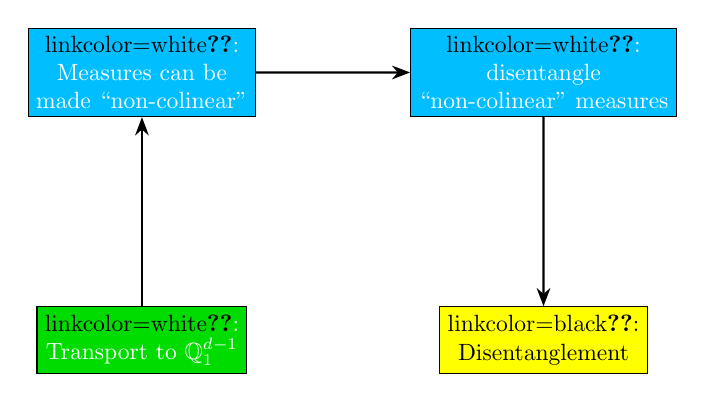
\begin{tikzpicture}[node distance=4cm, scale=0.85, every node/.style={transform shape}]

    % Define block styles
    \tikzset{
        section/.style={rectangle, minimum width=3cm, minimum height=1cm, text centered, draw=black, fill=#1},
        arrow/.style={thick, ->, >=Stealth}
    }

    % Nodes
    \node (1) [section=vibrantgreen, align=center] {\hypersetup{linkcolor=white}\Cref{lem: first.quadrant}\color{white}:\\ \color{white}Transport to $\mathbb{Q}_1^{d-1}$};
    \node (2) [section=skyblue, above of=1, align=center] {\hypersetup{linkcolor=white}\Cref{lem: perturbation}\color{white}:\\ \color{white}Measures can be\\ \color{white}made ``non-colinear''};
    \node (3) [section=skyblue, right of=2, xshift=2cm, align=center] {\hypersetup{linkcolor=white}\Cref{lem: induction.barycenter}\color{white}:\\ \color{white}disentangle\\ \color{white}``non-colinear'' measures};
    \node (6) [section=brightyellow, below of=3, align=center] {\hypersetup{linkcolor=black}\Cref{prop: separation}:\\Disentanglement};

    % Arrows
    \draw [arrow] (1) -- (2);
    \draw [arrow] (2) -- (3);
    %\draw [arrow] (3) -- (5);
    %\draw [arrow] (4) -- (5);
    \draw [arrow] (3) -- (6);

    \end{tikzpicture}
    \caption{High-level overview of the proof of \Cref{prop: separation}.}
    \label{fig: overview.1}
\end{figure}

\subsection{\texorpdfstring{Transportation to $\mathbb{Q}_1^{d-1}$}{Transportation to}}


By virtue of the following lemma, working with initial measures supported on $\mathbb{Q}_1^{d-1}$ is without loss of generality.

\begin{lemma} \label{lem: first.quadrant}
Let $T>0$. Suppose that $\mu_0^i\in\mathscr{P}(\S)$, for $i\in[N]$, are such that 
\begin{equation*}
    \bigcup_{i\in[N]} \mathrm{supp}(\mu^i_0)\subset\S.
\end{equation*}
Then there exists $\theta=(\bW,\bU,\bB,\bV,b)\in L^\infty((0,T);\Uptheta)$ such that 
\begin{equation*}
\mathrm{supp}(\mu^i(T)) \subset \mathbb{Q}_1^{d-1}
\end{equation*}
for all $i\in[N]$ where $\mu^i\in \mathscr{C}^0([0,T];\mathscr{P}(\S))$ denotes the unique solution to \eqref{eq: cauchy.pb} corresponding to $\mu_0^i$ and $\theta$.

Furthermore, one can take $\bV\equiv\bB\equiv\bU\equiv0$, $b\equiv{\bf 1}$, and $\bW$ piecewise constant, having at most one switch, and satisfying
\begin{equation*}
\|\bW\|_{L^\infty((0,T);\mathscr{M}_{d\times d}(\R))}\leq \frac{C}{T},
\end{equation*}
where $C>0$ depends only on the supports of the measures $\mu_0^i$, $i\in[N]$.
\end{lemma}

\begin{proof}[Proof of \Cref{lem: first.quadrant}]

Set $\bV\equiv \bB\equiv \bU\equiv 0$ and $b\equiv{\bf 1}$.

We begin by noting that by assumption, there exists some $\omega\in\S$ with $\omega\notin\mathrm{supp}(\mu_0^i)$ for all $i\in[N]$.
Let $T_0\in(0,T)$ be chosen later on. We select 
\begin{equation*}
    \bW(t)\equiv \bW_1 \hspace{1cm} \text{ for } t\in[0, T_0]
\end{equation*}
where $\bW_1$ is any $d\times d$ matrix such that
\begin{equation*}
\bW_1 {\bf 1}=-\omega.
\end{equation*}
For this choice of parameters, the characteristics of \eqref{eq: cauchy.pb} read
\begin{equation}\label{eq:EasyCircle}
\begin{dcases}
\dot{x}(t)=\proj_{x(t)}(-\omega) &\text{ in }[0, T_0]\\
x(0)=x_0.
\end{dcases}
\end{equation}
For any $x_0\in\S\setminus\{\omega\}$, we observe that the solution to \eqref{eq:EasyCircle} converges to $-\omega$ in long time. Indeed,
\begin{equation}\label{eq:BasicDissipation}
    \frac{\diff}{\diff t}\langle x(t), \omega\rangle=-1+\langle x(t),\omega \rangle^2<0 
\end{equation}
whenever $x(t)\in\S\backslash\{\pm\omega\}$. The solution to \eqref{eq:EasyCircle} defines a Lipschitz-continuous flow map 
$$\Phi^t\colon\S\to\S,$$ 
which is independent of any measure, and which allows to write the solution $\mu^i(t,\cdot)$ to \eqref{eq: cauchy.pb} on $[0, T_0]$ as
\begin{equation*}
    \mu^i(t)=\Phi^t_\#\mu_{0}^i
\end{equation*} 
for $i\in[N]$. Since $\omega$ does not belong to the support of any of the measures $\mu_0^i$, by virtue of \eqref{eq:BasicDissipation}, we can choose $T_0>0$, depending on
\begin{equation*}
    \min_{x\in \bigcup_{i\in[N]}\supp(\mu_0^i)}d_g(x,\omega)
\end{equation*}
so that
\begin{equation*} 
    \max_{x\in \supp(\mu^i(T_0))}d_g(x,-\omega)\leq \frac\pi8
\end{equation*}
for all $i\in[N]$.

Let $\alpha\in\mathbb{Q}_1^{d-1}$ be such that
\begin{equation*}
  d_g(-\omega,-\alpha)>\frac\pi8.  
\end{equation*}
As a consequence, $-\alpha$ does not belong to the support of $\mu^i(T_0)$ for any $i\in[N]$. Now we choose 
\begin{equation*}
    \bW(t)\equiv \bW_2 \hspace{1cm} \text{ for } t\in[T_0,T]
\end{equation*} 
where $\bW_2$ is any $d\times d$ matrix such that
\begin{equation*}
    \bW_2{\bf 1}=\alpha.
\end{equation*}
The characteristics of \eqref{eq: cauchy.pb} in $[T_0,T]$ then read
\begin{equation*}
\begin{cases}
       \dot{x}(t)=\proj_{{x(t)}}(\alpha) &\text{ in }[T_0, T]\\
x(T_0)=x_0.
\end{cases}
\end{equation*}
This differential equation defines a Lipschitz-continuous flow map 
$$\Psi^{t-T_0}:\S\to\S$$ 
with the same properties as in Step 1 (just replacing $-\omega$ by $\alpha$), i.e., we can choose $T>0$ large enough so that
\begin{equation*}
\mu^i(T)=\Big(\Psi^{T-T_0}\circ\Phi^{T_0}\Big)_\#\mu_{0}^i
\end{equation*}
satisfies
\begin{equation*}
    \supp(\mu^i(T))\subset \Q_1^{d-1}
\end{equation*}
for all $i\in[N]$, as desired. The bound on $\bW$ follows by rescaling time. \qedhere
\end{proof}


\subsection{A pair of lemmas}

The proof of \Cref{prop: separation} is based on the following lemmas.

\begin{lemma} \label{lem: induction.barycenter} 
Let $\mu_0^i\in\mathscr{P}(\Q_1^{d-1})$, $i\in[N]$, be given such that
    \begin{equation*}
        \mathbb{E}_{\mu_0^i}[x] \text{ is not colinear with }\mathbb{E}_{\mu_0^j}[x] \hspace{1cm} \text{ for } i\neq j.
    \end{equation*}
    Fix $j\in[N]$.
    Then for any $T>0$ and $\varepsilon>0$, and for any $\nu_0\in \mathscr{P}(\Q_1^{d-1})$ such that $\mathbb{E}_{\nu_0}[x]$ is colinear with $\mathbb{E}_{\mu_0^N}[x]$, there exists $\theta\in L^\infty((0,T);\Uptheta)$ such that 
    \begin{equation*}
        \supp(\nu(T))\cup\supp(\mu^j(T))\subset B\left( \frac{\mathbb{E}_{\mu^j_0}[z]}{\left\|\mathbb{E}_{\mu^j_0}[z]\right\|},\varepsilon\right),
    \end{equation*}
    and
    \begin{equation*}
        \mu^i(T)=\mu^i_0
    \end{equation*}
    for $i\neq j\in[N]$, where $\mu^i, \nu \in \mathscr{C}^0([0,T];\mathscr{P}(\S))$ 
    denote the unique solution to \eqref{eq: cauchy.pb}--\eqref{eq: average.vf} corresponding to data $\mu_0^i$, $\nu_0$, and the parameters $\theta$.

Furthermore, one can take $\theta$ piecewise constant, having  $O(d\cdot N)$ switches.
\end{lemma}

We postpone the proof to {\bf \Cref{proof: induction.barycenter}}.


\begin{lemma}\label{lem: perturbation} \label{lem: colinearity}
Let $T>0$ and let $\mu_0,\nu_0\in\mathscr{P}(\Q_1^{d-1})$ be two different measures such that
\begin{equation*}
        \mathbb{E}_{\mu_0}[x]= \gamma_1 \mathbb{E}_{\nu_0}[x]
    \end{equation*}
    for some $\gamma_1\in(0,1]$.
\begin{enumerate}
    \item If $\gamma_1=1$, then, setting $\bV\equiv0$, there exist $\bW,\bU\in\mathscr{M}_{d\times d}(\R)$ and $b\in \mathbb{R}^d$ such that the unique solutions $\mu, \nu$ to \eqref{eq: cauchy.pb}--\eqref{eq: average.vf} corresponding to $\mu_0, \nu_0$ and these parameters, satisfy
\begin{equation*}
    \mathbb{E}_{\mu(T)}[x]\neq \mathbb{E}_{\nu(T)}[x].
\end{equation*}
Moreover the Lipschitz-continuous and invertible flow map $\Phi^T:\S\to\S$ induced by the characteristics of \eqref{eq: cauchy.pb}--\eqref{eq: average.vf} with these parameters satisfies
\begin{equation}\label{eq: identity.flow}
    \Phi^T(x)=x\hspace{1cm}\text{ for }x\in \S\setminus\left(\supp(\mu_0)\cup\supp(\nu_0)\right).
\end{equation}
\item If $\gamma\neq 1$, then, setting $\bB\equiv0$, there exist $(\bV,\bW,\bU)\in L^\infty((0,T);\mathscr{M}_{d\times d}(\mathbb{R})^3)$ and $b\in L^\infty((0,T);\mathbb{R}^d)$,  piecewise constant with at most $2$ switches, such that the unique solutions $\mu, \nu$ to \eqref{eq: cauchy.pb}--\eqref{eq: average.vf} corresponding to data $\mu_0, \nu_0$ and these parameters satisfy
\begin{equation*}
    \mathbb{E}_{\mu(T)}[x]\neq\gamma_2\mathbb{E}_{\nu(T)}[x]
\end{equation*}
for all $\gamma_2\in\mathbb{R}$. In fact, 
\begin{align*}
  \bV(t)&=I_d 1_{(0,T_*)}(t) &  
  \bW(t)&=\bW 1_{(T_*,T)}(t) \\ 
  \bU(t)&=\bU 1_{(T_*,T)}(t) &
  b(t)&=b 1_{(T_*,T)}(t)  
\end{align*}
for some $T_*\in (0,T)$ and $\bW, \bU\in \mathscr{M}_{d\times d}(\mathbb{R})$, $b\in \mathbb{R}^d$. Moreover the Lipschitz-continuous and invertible flow map $\Phi^T:\S\to\S$ induced by the characteristics
\begin{equation*}
\begin{cases}
    \dot{x}(t)=\proj_x(\bW(t)(\bU(t) x+b(t))_+) &\text{ in } [0,T]\\
    x(0)=x\in\S,
\end{cases}    
\end{equation*}
satisfies
\begin{equation*}
  \Phi^T(x)=x\hspace{1cm} \text{ for all }x\notin \conv_g\, \supp(\mu_0)\cup \conv_g\, \supp(\nu_0).
\end{equation*}
\end{enumerate}
\end{lemma}

We postpone the proof to {\bf\Cref{proof: perturbation}}.






%\subsection{Proof of \Cref{prop: separation}}
\subsection{\texorpdfstring{Proof of \Cref{prop: separation}}{Proof of Proposition}} \label{sec: proof.prop.separation}


\begin{proof}[Proof of \Cref{prop: separation}]

We argue by induction over $N$. The base case $N=1$ is trivially satisfied. Assume that 
\begin{equation}\label{eq: empty.inter.sup}
\conv_g\,\supp(\mu^i_0)\cap\conv_g\,\supp(\mu^j_0)=\varnothing \hspace{1cm} \text{ for } i\neq j\in[N-1],
\end{equation}
and let $\mu_0^N\in \mathscr{P}(\Q_1^{d-1})$ be arbitrary. 
We prove that there exist parameters $\theta$ as in the statement, such that the solution $\mu^i$ to \eqref{eq: cauchy.pb} satisfies
\begin{equation*}
\supp(\mu^i(T))\cap\supp(\mu^j(T))=\varnothing\hspace{1cm} \text{ for } i\neq j\in[N].
\end{equation*}
Since $\supp(\mu^i_0)\subset\Q_1^{d-1}$, \eqref{eq: empty.inter.sup} implies that
\begin{equation*}
    \mathbb{E}_{\mu^i_0}[x]\text{ is not colinear with }\mathbb{E}_{\mu^j_0}[x] \hspace{1cm} \text{ for } i\neq j\in[N-1].
\end{equation*}
Now if $\mathbb{E}_{\mu_0^N}[x]$ is not colinear with $\mathbb{E}_{\mu_0^i}[x]$ for all $i\in[N-1]$, one can conclude by a simple application of \Cref{lem: induction.barycenter}. 
On another hand, as a consequence of \eqref{eq: empty.inter.sup}, $\mathbb{E}_{\mu^N_0}[x]$ is colinear with $\mathbb{E}_{\mu^i_0}[x]$ for at most one $i\in[N-1]$. 
Suppose that this is the case, and without loss of generality, we label this index $i=N-1$. We now proceed as follows.
\begin{enumerate}
    \item In $\left[0,T/4\right]$, we apply \Cref{lem: induction.barycenter}, with $\varepsilon>0$ small enough, to guarantee the existence of piecewise constant $\theta_1\in L^\infty((0,T/4); \Uptheta)$ having $O(d\cdot N)$ switches, such that the solution to \eqref{eq: cauchy.pb} satisfies
\begin{align}
    \supp\left(\mu^j\left(\frac{T}{4}\right)\right)\cap \supp\left(\mu^N\left(\frac{T}{4}\right)\right)=\varnothing\label{eq: first.step}\\
    \supp\left(\mu^j\left(\frac{T}{4}\right)\right)\cap \supp\left(\mu^{N-1}\left(\frac{T}{4}\right)\right)=\varnothing\nonumber
\end{align}
  for all $j\in[N-2]$.
\item In $\left[T/4,T/2\right]$, we apply the first part of \Cref{lem: perturbation} to find constant $\theta_2$ such that 
\begin{equation*}
    \mathbb{E}_{\mu^{N-1}\left(\frac{T}{2}\right)}[x]\neq \mathbb{E}_{\mu^{N}\left(\frac{T}{2}\right)}[x],
\end{equation*}
whereas, thanks to \eqref{eq: identity.flow} and the Lipschitz character of the ODE,
\begin{equation*}
    \supp\left(\mu^j\left(\frac{T}{2}\right)\right)\cap \supp\left(\mu^{N-1}\left(\frac{T}{2}\right)\right)=\varnothing
\end{equation*}
for all $j\in[N-2]$.
\item 
In $[T/2,3T/4]$, we apply the second part of \Cref{lem: colinearity} to $\mu^{N-1}\left(T/2\right)$ and $\mu^{N}\left(T/2\right)$ so that there are some piecewise constant $\theta_3\in L^\infty((T/2,3T/4);\Uptheta)$ such that 
\begin{equation*}
    \mathbb{E}_{\mu^N\left(\frac{3T}{4}\right)}[x] \text{ is not colinear with } \mathbb{E}_{\mu^{N-1}\left(\frac{3T}{4}\right)}[x].
\end{equation*}
Furthermore, owing to \eqref{eq: first.step}, and noting that $\bV=I_d$ in \Cref{lem: perturbation}, along with \eqref{eq: set.inclusion}, we also have  
\begin{equation*}
    \supp\left(\mu^i\left(\frac{3T}{4}\right)\right)\cap\supp\left(\mu^j\left(\frac{3T}{4}\right)\right)=\varnothing
\end{equation*}
for all $i\neq j\in[N-1]$, and for all $i\in[N-2]$ and $j=N$. 
\item The assumption of \Cref{lem: induction.barycenter} is now fulfilled by all $N$ measures, so by picking $\varepsilon>0$ small enough and applying \Cref{lem: induction.barycenter} once again, this time in $\left[3T/4,T\right]$, the conclusion follows.\qedhere
\end{enumerate}
\end{proof}




 


\section{Matching discrete measures} \label{sec: neural.ode}

The goal of this section is to prove the following result.

\begin{proposition} \label{prop: interpolation.neural.ode}
Suppose $d\geq3$. Consider 
\begin{equation*} \tag{$\mathscr{D}$}
  \left(x_0^i,y^i\right)\in\S\times\S \hspace{1cm} \text{ for } i\in[M], 
\end{equation*}
with $x_0^i\neq x_0^j$ and $y^i\neq y^j$ for $i\neq j$, and suppose that for any $i\in[M]$, there exist $\gamma_i\in\S$ and $\varepsilon_i>0$ such that
\begin{equation*} 
\left\langle\gamma_i,x_0^i-y^i\right\rangle=0 \hspace{1cm} \text{ and } \hspace{1cm} 
x_0^j\notin H_{\varepsilon_i}^{\gamma_i}
\end{equation*}
for $j\neq i\in[N]$, where
\begin{equation*}
H_{\varepsilon_i}^{\gamma_i}:=\Big\{x\in \S\colon|\langle x,\gamma_i\rangle|\leq \varepsilon_i\Big\}.
\end{equation*}
Then for any $T>0$, there exists $\theta=(\bW,\bU,b)\in L^\infty((0,T);\mathscr{M}_{d\times d}(\R)^2\times\R^d)$, piecewise constant having at most $6M$ switches, such that for any $i\in[M]$, the solution $x^i(\cdot)\in \mathscr{C}^0([0,T];\S)$ to
\begin{equation} \label{eq: neural.ode.sphere}
\begin{cases}
\dot{x}^i(t)=\proj_x\left(\bW(t)\Big(\bU(t)x^i(t)+b(t)\Big)_+\right) &\text{ in } [0, T]\\
x^i(0)=x_0^i,
\end{cases}
\end{equation}
satisfies 
$$x^i(T)=y^i.$$
Moreover there exists some $C>0$, not depending on $\mathscr{D}$ nor $T$, such that
\begin{equation*}
\|\theta\|_{L^\infty((0,T);\Uptheta)}\leq \frac{C\cdot M}{\displaystyle T\min_{i\in[M]}\varepsilon_{i}}.
\end{equation*}
\end{proposition}


The proof of \Cref{prop: interpolation.neural.ode} follows directly from the following result, combined with a straightforward induction argument. 

\begin{proposition} \label{lem: induction.neural.ode}
Suppose $d\geq3$. Consider 
\begin{equation*} \tag{$\mathscr{D}$}
  \left(x_0^i,y^i\right)\in\S\times\S \hspace{1cm} \text{ for } i\in[M], 
\end{equation*}
with $x_0^i\neq x_0^j$ and $y^i\neq y^j$ for $i\neq j$, with $x_0^i=y^i$ for $i\in[M-1]$, and suppose that there exist $\gamma\in\S$ and $\varepsilon>0$ such that
\begin{equation*} 
\left\langle\gamma,x_0^M-y^M\right\rangle=0 \hspace{1cm} \text{ and } \hspace{1cm} 
x_0^i\notin H_{\varepsilon}^{\gamma}
\end{equation*}
for all $i\in[M-1]$. 
Then, for every $T>0$, there exist piecewise constant parameters $\theta=(\bW,\bU,b)\in L^\infty((0,T);\mathscr{M}_{d\times d}(\R)^2\times\R^d)$, all having at most $6$ switches, such that for any $i\in[M]$, the solution $x^i(\cdot)\in \mathscr{C}^0([0,T];\S)$ to \eqref{eq: neural.ode.sphere} satisfies
\begin{equation*}
x^i(T)=y^i.
\end{equation*}
Moreover, there exists some constant $C>0$, not depending on $\mathscr{D}$ and $T$, such that
    \begin{equation*}
        \|\theta\|_{L^\infty((0,T); \Uptheta)}\leq \frac{C}{T\cdot\varepsilon}.
    \end{equation*}
\end{proposition}

\begin{proof}[Proof of \Cref{lem: induction.neural.ode}]
The final parameters take the form
\begin{align*}
    \bW(t) &= \sum_{j=1}^6 \bW_j 1_{\left[\frac{(j-1)T}{6},\frac{jT}{6}\right]}(t),\\
    \bU(t) &= \sum_{j=1}^6 \bU_j 1_{\left[\frac{(j-1)T}{6},\frac{jT}{6}\right]}(t),\\
    b(t) &= \sum_{j=1}^6 b_j 1_{\left[\frac{(j-1)T}{6},\frac{jT}{6}\right]}(t),
\end{align*}
where 
\begin{align*}
  \bW_5 &= -\bW_1 & \bU_5 &= \bU_1 & b_5 &= b_1, \\
  \bW_6 &= -\bW_2 & \bU_6 &= \bU_2 & b_6 &= b_2, \\
         &         & \bU_3 &= \bU_4 & b_3 &= b_4.
\end{align*}
Throughout, the time \( T > 0 \) is adjusted later by rescaling the norm of the parameters.


%Moreover, in the construction we take $\bU_3=\bU_4$ and $b_3=b_4.$. On the other hand, we set $\bU_5=\bU_1$, $b_5=b_1$, $\bW_5=-\bW_1$, and $\bU_6=\bU_2$, $b_6=b_2$, $\bW_6=-\bW_2$.

\subsubsection*{Step 1. The anchor points}
In this step we find three anchor points which serve to build the parameters in what follows. 
Since $\langle \gamma, x_0^M-y^M\rangle=0$, we can find some $\omega\in\S$ such that 
\begin{equation}\label{eq: great.circle.hyperplane}
\langle \gamma, \omega\rangle=0,
\end{equation}
as well as
\begin{equation}\label{eq: omega.distance}
d_g\left(\omega, x_0^M\right)\geq \frac{\pi}{2},\hspace{1cm}\text{ and } \hspace{1cm}  d_g\left(\omega, y^M\right)\geq\frac{\pi}{2}.
\end{equation}
Because of \eqref{eq: great.circle.hyperplane}, we consider the point $\omega_+$ lying on the minimizing geodesic between $\omega$ and $\gamma$, satisfying
\begin{equation*}
d_g(\omega_+,\omega)=\frac{\pi}{8}.
\end{equation*}
Similarly, we consider the point $\omega_-$ lying on the minimizing geodesic between $\omega$ and $-\gamma$, satisfying 
\begin{equation*}
d_g(\omega_-,\omega)=\frac{\pi}{8}.
\end{equation*}
We have 
\begin{align*}
d_g\left(\omega_+,x_0^M\right)&\geq d_g\left(\omega,x_0^M\right)-d_g\left(\omega,\omega_+\right)=\frac{3\pi}{8},\\
d_g\left(\omega_+,y^M\right)&\geq \frac{3\pi}{8},\\ 
d_g\left(\omega_-,x_0^M\right)&\geq \frac{3\pi}{8},\\
d_g\left(\omega_-,y^M\right)&\geq \frac{3\pi}{8}.
\end{align*}
As a consequence, the hyperplane 
\begin{equation*}
\left\{x\in\S\colon\langle\omega,x\rangle=\cos\left(\frac{\pi}{8}+\tau\right)\right\}
\end{equation*}
is a separating hyperplane for the ball $B\left(\omega,\frac{\pi}{8}+\tau\right)$ and the points $x_0^M$ and $y^M$ for every $\tau\in(0,\frac{3\pi}{8})$; namely
\begin{equation*}
\left\langle \omega,x_0^M\right\rangle -\cos\left(\frac{\pi}{8}+\tau\right)=\cos d_g\left(\omega,x_0^M\right)-\cos\left(\frac{\pi}{8}+\tau\right)<0,
\end{equation*}
where the inequality is by virtue of \eqref{eq: omega.distance}. 
Analogous computations hold for $y^M$, whereas
\begin{equation*}
\langle\omega,x\rangle -\cos\left(\frac{\pi}{8}+\tau\right)>0
\end{equation*}
for all $x\in B(\omega,\frac{\pi}{8}+\frac{1}{2}\tau)$ and $\tau\in(0,\frac{3\pi}{8})$ (see \Cref{fig: setup.ball}).

\begin{figure}[!ht]
    \centering
    \includegraphics[scale=0.75]{figures/figure-4.pdf}
    \caption{The geometric configuration of Step 1.}
    \label{fig: setup.ball}
\end{figure}
            
\subsubsection*{Step 2. Isolating $x_0^M$ and $y^M$} 
Let 
$$\epsilon:=\min\left\{\varepsilon,\frac{\pi}{4}\right\}.$$ 
Consider 
\begin{equation*}
 \bU_1=\gamma {\bf1}^\top \hspace{1cm} \text{ and } \hspace{1cm}   b_1=-\frac{\epsilon}{2}{\bf1}. 
\end{equation*}
Then
\begin{equation*}
\left(\bU_1x+b_1\right)_+=\left(\langle \gamma, x\rangle -\frac{\epsilon}{2}  \right)_+{\bf1}.
\end{equation*}
Choose any $\bW_1$ so that
\begin{equation*}
\bW_1{\bf1}=\omega_+.
\end{equation*}
Define
\begin{equation*}
\mathscr{S}_+:=\left\{ x\in \S:\langle \gamma, x\rangle \geq \epsilon\right\}.
\end{equation*}
Obviously $\omega_+\in \mathscr{S}_+$. 
Observe that the trajectories of the ODE
\begin{equation} \label{eq: neural.ode.separation}
\dot{x}(t)=\left(\langle \gamma, x(t)\rangle -\frac{\epsilon}{2}\right)_+\proj_{x(t)}(\omega_+)\hspace{1cm}\text{ for $t\geq0$,}
\end{equation}
follow the Riemannian gradient flow of the distance between $\omega_+$ and $x$ in $\mathscr{S}_+$. Indeed,
\begin{equation*}
     \nabla_1 d_g(x,\omega_+)=-\frac{\proj_x(\omega_+)}{\sqrt{1-\langle x,\omega_+\rangle^2 }}.
\end{equation*}
Then, setting $f(x)=\left(\langle \gamma, x\rangle -\frac{\epsilon}{2}\right)_+$, we have
 \begin{align*}
    \dot{x}(t)&=-f(x(t))\,\sqrt{1-\langle x(t),\omega_+\rangle^2 } \,\nabla_1 d_g(x(t),\omega_+)\nonumber\\
    &=-\overline{f}(x(t))\,\nabla_1 d_g(x(t),\omega_+).
 \end{align*}
 Since $\overline{f}$ is a nonnegative scalar function, by appropriately reparameterizing time, we conclude that $x(t)$ follows the desired gradient flow.
 In turn, the trajectory $x(t)$ of \eqref{eq: neural.ode.separation} starting from any $x_0\in\mathscr{S}_+$ always lies on the minimal geodesic from $x_0$ to $\omega_+\in\mathscr{S}_+$. Since $\mathscr{S}_+$ is geodesically convex, we gather that $x(t)\in\mathscr{S}_+$ for all $t\geq0$. Then, notice that 
 \begin{equation*}
     \overline{f}(x)=0 \qquad \Longleftrightarrow \qquad x=\omega_+ \quad \text{ or } \quad x\in  \left\{y\in\S:\langle \gamma,y\rangle\leq \frac{\epsilon}{2}\right\}.
 \end{equation*}
 Thus, unless $x(t)=\omega_+$, $\overline{f}$ is uniformly bounded from below on $\mathscr{S}_+$, and since 
 \begin{equation*}
     \nabla_1 d_g(x,\omega_+)=0 \qquad \Longleftrightarrow \qquad x=\pm \omega_+,
 \end{equation*}
 we can conclude that $x(t)\to\omega_+$ as $t\to+\infty$ for any $x_0\in\mathscr{S}_+$ by applying the LaSalle invariance principle \cite{lasalle1960some}.
 
% {\color{red} Therefore \eqref{eq: gradient.flow} allows to say that, given $x_0\in \mathscr{S}_+$, the solution to \eqref{eq: neural.ode.separation}, $x(t)$ lies on the minimal geodesic $\gamma$ starting at $x_0$ and ending at $\omega_+$, i.e.
% \begin{equation}\label{eq: trajectory.geodesic}
%     x(t)\in \left\{y\in \S:\,  y=\gamma(s), \text{ for some }s\in [0,1]\right\}\text{ for all }t\geq 0.
% \end{equation}
% Since $\mathscr{S}_+$ is geodesically convex, \eqref{eq: trajectory.geodesic} implies that for every $x_0\in \mathscr{S}_+$, the solution to \eqref{eq: neural.ode.separation} satisfies $x(t)\in \mathscr{S}_+$ is invariant by the flow generated by \eqref{eq: neural.ode.separation} and, furthermore, since 
% \begin{equation*}
%     \overline{f}(x)=0\Longleftrightarrow x=\omega_+\text{ or }x\in  \left\{y\in\S:\langle \gamma,y\rangle-\frac{\epsilon}{2}\leq 0\right\}
% \end{equation*}
% and $f(x)$ is uniformly bounded from below on $\mathscr{S}_+$, 
% and furthermore
% \begin{equation*}
%     \nabla d_g(x,\omega_+)=0 \Longleftrightarrow x=\pm \omega_+
% \end{equation*}
% therefore, by LaSalle's invariance principle \cite{lasalle1960some}, we have $x(t)\to\omega_+$ as $t\to+\infty$ for all $x_0\in \mathscr{S}_+$.
% }

For any $x_0\in\S$, set
\begin{equation*}
T_{\frac{\pi}{16}}(x_0):=\inf\left\{t\geq 0:\quad x(t)\in B\left(\omega_+,\frac{\pi}{16}\right)\right\},
\end{equation*}
where $x(\cdot)$ is the solution to the Cauchy problem for \eqref{eq: neural.ode.separation} with data $x_0$. 
Since $\|\gamma\|=1$, $\|\bW_1\|_{\text{op}}\leq1$ and $\|b_1\|\leq\frac{\epsilon}{2}\sqrt{d}$, bounding the $L^\infty$--norm of the parameters comes from bounding $T_{\frac{\pi}{16}}(x_0)$ uniformly over $x_0\in\mathscr{S}_+$ and rescaling time. 
For every $x_0\in B\left(\omega_+,\frac{\pi}{16}\right)$ we see that $T_{\frac{\pi}{16}}(x_0)$ is trivially $0$, whereas for  $x_0\in \mathscr{S}_+\setminus B\left(\omega_+,\frac{\pi}{16}\right)$ one has
\begin{align} \label{eq: estimate.neural}
\frac{\diff}{\diff t} \langle x(t),\omega_+\rangle&=\left( \langle \gamma, x(t)\rangle-\frac{\epsilon}{2}\right)_+\left(1-\langle \omega_+,x\rangle^2\right)\nonumber\\
&\geq \frac{\epsilon}{2}\left(1-\langle \omega_+,x\rangle^2\right)\nonumber\\
&\geq \frac{\epsilon}{2}\left(1-\cos^2\left(\frac{\pi}{16}\right)\right).
\end{align}
Hence $T_{\frac{\pi}{16}}(x_0)=O(1/\epsilon)$ for all $x_0\in \mathscr{S}_+$.  

Finally, by following the same arguments leading to \eqref{eq: estimate.neural}, beyond some large enough time, and for every $x_0\in \mathscr{S}_+$, we can apply the Hartman-Grobman theorem \cite{hartman1960lemma, hartman1963local, shub2013global}: the behavior near the critical point $\omega_+$ is governed\footnote{Note that the critical point $\omega_+$ is hyperbolic since we are working in $\mathsf{T}_{\omega_+}\S$. On $\mathbb{R}^d$, there is a zero eigenvalue associated to the radial direction.} by the linearized system 
 \begin{equation*}
 \begin{cases}
     \dot{y}(t)=-\left(\langle \gamma,\omega_+\rangle-\displaystyle\frac{\epsilon}{2}\right)y(t) & \text{ in } \R_{\geq0}\\
     y(0)=y_0\in \mathsf{T}_{\omega_+}\S,
     \end{cases}
 \end{equation*}
 which is exponentially stable. Thus, by the Hartman-Grobman theorem, for all $x_0\in\mathscr{S}_+$,
 \begin{equation}\label{eq: Hartman.Grobman}
     d_g(x(t),\omega_+)\leq Ke^{-\lambda t} \hspace{1cm} \text{  for all } t\geq 0, 
 \end{equation}
and for some $\lambda>0$ and $K\geq 1$ which depend on $x_0$, $\epsilon$ and $\gamma$ only.

Similarly, consider 
\begin{equation*}
 \bU_2=-\gamma {\bf1}^\top \hspace{1cm} \text{ and } \hspace{1cm}   b_2=-\frac{\epsilon}{2}{\bf1}.
\end{equation*}
Then, 
\begin{equation*}
(\bU_2x+b_2)_+=\left( \langle -\gamma, x\rangle -\frac{\epsilon}{2}\right)_+ {\bf1}.
\end{equation*}
Choose any $\bW_2$ so that
\begin{equation*}
\bW_2{\bf1}=\omega_-.
\end{equation*}
Define
\begin{equation*}
\mathscr{S}_-:=\left\{ x\in \S:    \langle -\gamma, x\rangle \geq \epsilon\right\}.
\end{equation*}
After reasoning similarly for $\mathscr{S}_-$ as for $\mathscr{S}_+$, and by rescaling time so that
\begin{equation*}
\|\bW_1\|_{\text{op}} = O\left( \frac{1}{T\cdot\epsilon}\right), \qquad \|\bW_2\|_{\text{op}}=O\left( \frac{1}{T\cdot\epsilon}\right),
\end{equation*}
we deduce that for any $T>0$ there exists $\theta_1\in L^\infty((0,T/3);\mathscr{M}_{d\times d}(\mathbb{R})^2\times \mathbb{R}^d)$, piecewise constant having two switches, such that the associated flow map of \eqref{eq: neural.ode.sphere} is a Lipschitz-continuous and invertible map that satisfies
\begin{align}\label{eq: sphere.separation}
&\Phi^{\frac{T}{3}}_{\theta_1}(x_0^i)\in B\left(\omega,\frac{3\pi}{16}\right)\\
&\Phi^{\frac{T}{3}}_{\theta_1}(x)=x\hspace{1cm}\text{ if }x\in H_\epsilon^\gamma\nonumber.
\end{align}

\begin{figure}
    \centering
        \includegraphics[scale=0.6]{figures/figure-5.pdf}
    \hspace{0.5cm}
        \includegraphics[scale=0.6]{figures/figure-6.pdf}
    \caption{({\it Left}) All points in one spherical cap converge to $\omega_+$. ({\it Right}) All points aside the $M$-th one are in a neighbourhood of $\omega_+$ or $\omega_-$. Consequently there is a separating hyperplane between $x_0^M$ and $y^M$ (dashed).}
    \label{fig:?}
\end{figure}

\subsubsection*{Step 3. Steering $x_0^M$ to $y^M$}




By virtue of \eqref{eq: sphere.separation}, the hyperplane
\begin{equation*}
\left\{x\in\S\colon\langle \omega, x\rangle =\cos\left(\frac{3\pi}{16}\right)\right\}
\end{equation*}
is a separating hyperplane: it separates $x_0^N$ and $y^N$ from $\Phi_{\theta_1}^{\frac{T}{3}}(x_0^i)$ for $i\in[M-1]$. Consider
\begin{align*}
\bU_3=-\omega {\bf1}^\top, \hspace{1cm} \text{ and } \hspace{1cm}
b_3=\cos\left(\frac{3\pi}{16}\right){\bf1}.
\end{align*}
With this choice, we have 
\begin{align*}
    \left( \bU_3x+b_3 \right)_+=0 \hspace{1cm} \text{ for } &x\in B\left(\omega, \frac{3\pi}{16}\right),\\
    \left( \bU_3x+b_3 \right)_+= \underbrace{\left(\langle -\omega, x\rangle+\cos\left(\frac{3\pi}{16}\right)\right)}_{>0} {\bf1} \hspace{1cm} \text{ for } &x\in \S\setminus B\left(\omega, \frac{3\pi}{16}\right).
\end{align*}
Take two points $z_1,z_2\in \S\setminus B\left(\omega, \frac{3\pi}{16}\right)$ such that
\begin{enumerate}
    \item $\{c(s)\}_{s\in[0,1]}$ is a geodesic satisfying $c(0)=x_0^M$ and $c(1)=z_2$;
    \item $c(1-s_0)=y^M$ for some $s_0\in(0,1)$;
    \item $c(s_{z_1})=z_1$ for some $s_{z_1}\in(0,1-s_0)$;
    \item $\{c(s)\}_{s\in[0,1]}\subset \S\setminus B\left(\omega, \frac{3\pi}{16}\right)$;
    \item $d_g(z_1,x_0^M)\leq \kappa\pi$ and $d_g(z_1,z_2)\leq \kappa\pi$ for some\footnote{can be chosen as such because $\{c(s)\}_{s\in[0,1]}\subset \S\setminus B\left(\omega,\frac{3\pi}{16}\right)$---indeed, take $\kappa=\frac{29}{32}$.} $\kappa<1$.
\end{enumerate}
Consider any $d\times d$ matrix $\bW_3$ such that
\begin{equation*}
\bW_3{\bf1}=z_1.
\end{equation*}
The Cauchy problem \eqref{eq: neural.ode.sphere} with these parameters, for the $i=M$-th particle, reads
\begin{equation}\label{eq: neural.ode.step3}
\begin{cases}
\dot{x}(t)=\left(\langle -\omega, x(t)\rangle+\cos\left(\frac{3\pi}{16}\right)\right)_+\proj_{x(t)}(z_1) &\text{ on } \R_{\geq0}\\
x(0)=x_0^M.
\end{cases}
\end{equation}
Since $d_g(x_0^M,z_1)\leq\kappa\pi$, and since the minimizing geodesic between $x_0^M$ and $z_1$ is contained in $\{c(s)\}_{s\in [0,1]}\subset B(\omega, \frac{3\pi}{16})$, we gather that there exists some large enough time $\tau>0$ such that
\begin{equation} \label{eq: geodesic.toll}
    d_g\left( x(\tau),z_2\right)\leq d_g\left( x(\tau),z_1\right)+d_g\left( z_1,z_2\right)\lesssim e^{-\lambda\tau}+\kappa\pi\leq\kappa_2\pi
\end{equation}
for some $\kappa_2<1$ and $\lambda>0$. This comes from the long-time convergence of \eqref{eq: neural.ode.step3} to $z_1$, which can be shown by following the same arguments as for \eqref{eq: Hartman.Grobman}, replacing $\omega_+$ by $z_1$. 
For any $d\times d$ matrix $\bW_4$ such that
\begin{equation*}
\bW_4{\bf1}=z_2,
\end{equation*}
the Cauchy problem \eqref{eq: neural.ode.sphere}, for the $i=M$-th particle, reads
\begin{equation} \label{eq: neural.ode.step3.2}
\begin{cases}
\dot{x}(t)=\left(\langle -\omega, x(t)\rangle+\cos\left(\frac{3\pi}{16}\right)\right)_+\proj_{x(t)}(z_2) &\text{ for } t\geq\tau\\
x(\tau) = x(\tau)
\end{cases}
\end{equation}
where $x(\tau)$ is the solution of \eqref{eq: neural.ode.step3} at $t=\tau$. Since $d_g(z_1,z_2)\leq \kappa \pi$, $y^M$ lies on the minimizing geodesic between $x(\tau)$ and $z_2$. All the while, thanks to \eqref{eq: geodesic.toll}, taking $T$ even larger than before, we deduce that that the solution to \eqref{eq: neural.ode.step3.2} satisfies
\begin{equation*}
    x(T)=y^M.
\end{equation*}
Therefore, as in the previous step, we deduce that for any $T>0$ there exists some $\theta_2\in L^\infty((T/3,2T/3);\mathscr{M}_{d\times d}(\mathbb{R})^2\times\mathbb{R}^d)$, piecewise constant having two switches, such that the associated flow map of \eqref{eq: neural.ode.sphere} is a Lipschitz-continuous and invertible map that satisfies
\begin{align*}
\Phi^{\frac{2T}{3}}_{\theta_2}(x)&=x\hspace{1cm}\text{ if }x\in B\left(\omega, \frac{3\pi}{16}\right),\\
\Phi^{\frac{2T}{3}}_{\theta_2}(x_0^M)&=y^M,
\end{align*}
and
\begin{equation*}
    \left(\Phi_{\theta_2}^{\frac{2T}{3}}\circ\Phi_{\theta_1}^{\frac{T}{3}}\right)(x_0^i)= \Phi_{\theta_1}^{\frac{T}{3}}(x_0^i)\in B\left(\omega, \frac{3\pi}{16}\right)\qquad\text{ for } i\in[M-1]
\end{equation*}
as well as
\begin{equation*}
    \left(\Phi_{\theta_2}^{\frac{2T}{3}}\circ\Phi_{\theta_1}^{\frac{T}{3}}\right)(x_0^M)= \Phi_{\theta_2}^{\frac{2T}{3}}(x_0^M)=y^M.
\end{equation*}


\subsubsection*{Step 4. Bringing $x^i(T)$ back to $y^i$}
We conclude by applying the inverse of the flow map $\Phi^{\frac{T}{3}}_{\theta_1}$: defining
\begin{equation*}
    \Phi^T_{\text{fin}}:=\left(\Phi^{\frac{T}{3}}_{\theta_1}\right)^{-1}\circ \Phi^{\frac{2T}{3}}_{\theta_2} \circ\Phi^{\frac{T}{3}}_{\theta_1},
\end{equation*}
we have $\Phi^T_{\text{fin}}(x_0^i)=y^i$ for all $i\in[M]$, as desired.
\end{proof}


\begin{remark}
\Cref{prop: compression} yields a flow map that clusters the support of the input measure, which in turn allows to reduce a universal approximation property of maps in $L^p(\S;\S)$ to interpolation via flow maps  proved in \Cref{prop: interpolation.neural.ode}. 
Indeed it suffices to consider a simple function $\varphi:\S\to\S$ defined as
\begin{equation*}
\varphi(x)=\sum_{i=1}^N y_i1_{\Omega_i}(x)
\end{equation*}
with $y_i\in \S$. Universal approximation in $L^p(\S;\S)$, $p<+\infty$, is equivalent to the $\mathsf{W}_p$-approximate interpolation of
\begin{equation*}
\diff\mu_0^i(x)=1 _{\Omega_i}(x)\diff x,\quad
\mu_1^i=|\Omega_i|\updelta_{y_i}
\end{equation*}
for $i\in[N]$. Note that, by construction, the supports of $\mu_0^i$ (and of $\mu_1^i$) are pairwise disjoint. Thus the attention component of the vector field is not needed to perform this task. This is generalized in the next section.
\end{remark}



\section{Proofs of the main results} \label{sec: proofs}

Our overarching goal is to construct the solution map $\Phi_{\mathrm{fin}}^T:\mathscr{P}(\S)\to\mathscr{P}(\S)$ of the form
$$\Phi_{\mathrm{fin}}^T:=\left(\Phi^{\frac{T}{3}}_{\theta_3}\right)^{-1}\circ \Phi^{\frac{T}{3}}_{\theta_2}\circ \Phi^{\frac{T}{3}}_{\theta_1}, 
$$
where $$\Phi_{\theta_1}^{\frac{T}{3}}=:\Phi_1$$ and 
$$\Phi_{\theta_3}^{\frac{T}{3}}=:\Phi_3$$ 
are the flow maps given by \Cref{prop: separation}, so that the measures $\Phi_1(\mu_0^i)$ (and $\Phi_3(\mu_1^i)$), for $i\in[N]$, have pairwise disentangled supports. The map 
$$\Phi_{\theta_2}^{\frac{T}{3}}=:\Phi_2$$ 
is constructed in this section (see \Cref{fig: overview.2} for a schematic overview of the entire proof). The main clue lies in the following three lemmas.

\begin{lemma}[Propagating transport maps]
\label{lem: hyp.propagation}
Suppose that for every $i\in[N]$ there exists $\mathsf{T}^i\in L^2(\S;\S)$ such that
\begin{equation} \label{eq: hypothesis}
    \mathsf{T}^i_\#\mu_0^i=\mu_1^i.
\end{equation}
Consider the flow map $\Phi_1:\mathscr{P}(\S)\to\mathscr{P}(\S)$ (respectively $\Phi_3$) given by \Cref{prop: separation} with data $\mu_0^i\in\mathscr{P}(\S)$ (respectively $\mu_1^i\in\mathscr{P}(\S)$) for $i\in[N]$. 
Then, there exists a Lipschitz-continuous and invertible map $\Psi:\S\to\S$ such that
\begin{equation} \label{eq: diffeo.supports}
\Psi\big|_{\supp\left(\Phi_1(\mu_0^i)\right)}=\Psi^i
\end{equation}
for any $i\in[N]$, where $\Psi^i:\S\to\S$ is another Lipschitz-continuous and invertible map that satisfies
\begin{equation*}
\left(\Psi^i\circ \mathsf{T}^i_{\Phi_1}\right)_\#\mu_0^i= \left(\Psi\circ \mathsf{T}^i_{\Phi_1}\right)_\#\mu_0^i=\left(\mathsf{T}^i_{\Phi_3}\right)_\#\mu_1^i=\Phi_3(\mu_1^i)
\end{equation*}
for some Lipschitz-continuous and invertible maps $\mathsf{T}_{\Phi_1}^i, \mathsf{T}_{\Phi_3}^i:\S\to\S$.
\end{lemma}

The proof can be found in {\bf \Cref{proof: hyp.propagation}}.

\begin{lemma}
\label{lem: monge}
Suppose $\mu\in \mathscr{P}(\S)$ and $\mathsf{T}^1,\mathsf{T}^2:\S\to\S$ measurable, with $\mathsf{T}^1$ bijective. Then
\begin{equation} \label{eq: linearized.wasserstein}
\mathsf{W}_2\left(\mathsf{T}^1_\#\mu,\mathsf{T}^2_\#\mu\right)\lesssim\left\|\mathsf{T}^1-\mathsf{T}^2\right\|_{L^2(\mu)}.
\end{equation}
\end{lemma}

The proof is elementary, but brief, thus we provide it for completeness.

\begin{proof}[Proof of \Cref{lem: monge}]
Since $\mathsf{T}^1$ is bijective, there is a measurable $\Psi:\S\to \S$ such that
\begin{equation*}
\Psi(\mathsf{T}^1(x))=\mathsf{T}^2(x) \hspace{1cm} \text{ for all } x\in\S. 
\end{equation*}
Then
\begin{equation*}
\mathsf{W}_2^2\left(\mathsf{T}^1_\#\mu,\mathsf{T}^2_\#\mu\right)\lesssim\int\|x-\Psi(x)\|^2\left(\mathsf{T}^1_\#\mu\right)(\diff x)=\left\|\mathsf{T}^1-\mathsf{T}^2\right\|_{L^2(\mu)}^2.\qedhere
\end{equation*}
\end{proof}

\begin{remark}
    When $\mu$ is absolutely continuous with respect to the Lebesgue measure, and
    $\mathsf{T}^1$ and $\mathsf{T}^2$ are the optimal transport maps between $\mu$ and $\nu_1$, and $\mu$ and $\nu_2$ respectively, the upper bound in \eqref{eq: linearized.wasserstein} is know as the \emph{linearized optimal transport distance} (see \cite{delalande2023quantitative, jiang2023algorithms} and the references therein).
\end{remark}

Finally,

\begin{lemma} \label{lem: univ.approx}
Suppose $\varepsilon>0$ and $\mu\in \mathscr{P}(\S)$. 
For every $\Psi\in L^2(\S;\S)$, there exists a Lipschitz-continuous and invertible map $\Psi_\varepsilon:\S\to\S$ induced by the solution map of \eqref{eq: neural.pde.sphere}, namely 
$$\Phi^T_{\theta_\varepsilon}(\mu)=(\Psi_\varepsilon)_\#\mu$$ for some piecewise constant $\theta_\varepsilon\in L^\infty((0,T);\Uptheta)$ with finitely many switches, such that
\begin{equation*}
\left\|\Psi-\Psi_\varepsilon\right\|_{L^2(\mu)}\leq\varepsilon.
\end{equation*}
\end{lemma}

The proof of \Cref{lem: univ.approx} is involved, so we postpone it to {\bf \Cref{proof: univ.approx}}.


\subsection{\texorpdfstring{Proof of \Cref{thm: main.result}}{Proof of Theorem}}

We provide \emph{two} proofs: we first provide the proof in full generality, followed by a simpler proof that doesn't rely on \Cref{lem: univ.approx}, under stronger structural assumptions on the input and target measures.


\begin{proof}[Proof of \Cref{thm: main.result} (general case)]

We split the proof in three steps.

\subsubsection*{Step 1. Disentanglement} 

We begin by rendering the supports of the initial measures $(\mu_0^i)_{i\in[N]}$ (respectively, the target measures $(\mu_1^i)_{i\in[N]}$) pairwise disjoint by virtue of applying \Cref{prop: separation} to \eqref{eq: cauchy.pb} with data $\mu_0^i$ at time $t=0$ (respectively $\mu_1^i$ at time $t=2T/3$) for any $i\in[N]$. 
This entails the existence of two parameterized flow maps
\begin{equation*}
    \Phi_{\theta_1}^{t}:\mathscr{P}(\S)\mapsto \mathscr{P}(\S)
\end{equation*}
for $t\in[0,T/3]$, and
\begin{equation*}
    \Phi_{\theta_3}^{t}:\mathscr{P}(\S)\mapsto \mathscr{P}(\S)
\end{equation*}
for $t\in[2T/3, T]$, induced by \eqref{eq: cauchy.pb}, which are such that
\begin{equation*}
    \supp\left(\Phi_{\theta_1}^{\frac{T}{3}}(\mu_0^i)\right)\cap \supp\left(\Phi_{\theta_1}^{\frac{T}{3}}(\mu_0^j)\right)=\varnothing\hspace{1cm}\text{ if }i\neq j,
\end{equation*}
and 
\begin{equation*}
    \supp\left(\Phi_{\theta_3}^{T}(\mu_1^i)\right)\cap \supp\left(\Phi_{\theta_3}^{T}(\mu_1^j)\right)=\varnothing\hspace{1cm}\text{ if }i\neq j.
\end{equation*}
Since \eqref{eq: cauchy.pb} is well-posed and time-reversible, %by using \cite[I think that 4 is enough for our purposes]{geshkovski2023emergence}
we further gather that there exists some constant $C=C(T,\theta_3)>0$ such that
\begin{equation} \label{eq: continuity.inverse.flow}
\mathsf{W}_2\left(\left(\Phi_{\theta_3}^{T}\right)^{-1}(\mu),\left(\Phi_{\theta_3}^{T}\right)^{-1}(\nu)\right)\leq C\cdot\mathsf{W}_{2}(\mu,\nu)
\end{equation}
holds for any $\mu,\nu\in \mathscr{P}(\S)$.


\subsubsection*{Step 2. Matching}


By virtue of \Cref{lem: hyp.propagation}, there exists a Lipschitz-continuous and invertible map $\Psi:\S\to \S$ such that 
\begin{equation*}
    \Psi\Big|_{\supp\left(\Phi^{\frac{T}{3}}_{\theta_1}(\mu_0^i)\right)}=\Psi^i,
\end{equation*}
for $i\in[N]$ where $\Psi^i:\S\to\S$ satisfies 
\begin{equation} \label{eq: first.psi}
    \Psi^i_\# \left(\Phi^{\frac{T}{3}}_{\theta_1}(\mu_0^i)\right)=\Phi^{\frac{T}{3}}_{\theta_3}(\mu_1^i).
\end{equation}
We consider
\begin{equation*}
    \mu=\sum_{i=1}^N \Phi_{\theta_1}^{\frac{T}{3}}(\mu_0^i),
\end{equation*}
and use \Cref{lem: univ.approx} to find a flow map $\Psi_\varepsilon:\S\to\S$ such that
\begin{equation} \label{eq: second.psi}
    \left\|\Psi^i-\Psi_\varepsilon\Big|_{\supp\left(\Phi_{\theta_1}^{\frac{T}{3}}(\mu_0^i)\right)}\right\|_{L^2\left(\Phi_{\theta_1}^{\frac{T}{3}}(\mu_0^i)\right)}\leq\|\Psi-\Psi_\varepsilon\|_{L^2(\mu)}\leq\frac{\varepsilon}{C}
\end{equation}
for $i\in[N]$. In fact by virtue of \Cref{lem: univ.approx} there exists a parameterized flow map
\begin{equation*}
    \Phi_{\theta_2}^{t}:\mathscr{P}(\S)\to \mathscr{P}(\S)
\end{equation*}
for $t\in[T/3,2T/3]$, induced by \eqref{eq: cauchy.pb} and defined, for $\nu\in \mathscr{P}(\S)$, as
\begin{equation*}
    \Phi_{\theta_2}^{\frac{2T}{3}}(\nu)=(\Psi_\varepsilon)_\#\nu,
\end{equation*}
which by virtue of \eqref{eq: first.psi}, \eqref{eq: second.psi} and \Cref{lem: monge}, satisfies
\begin{equation}\label{eq: gluing.flow}
    \mathsf{W}_2\left(\left(\Phi_{\theta_2}^{\frac{2T}{3}}\circ \Phi_{\theta_1}^{\frac{T}{3}}\right)(\mu_0^i),\Phi_{\theta_3}^{T}(\mu_1^i)\right)\leq\frac{\varepsilon}{C}
\end{equation}
for all $i\in[N]$.

\subsubsection*{Step 3. Continuity}

We now apply the inverse of $\Phi_{\theta_3}^{T}$ to conclude that
the map
\begin{equation*}
\Phi_{\text{fin}}^T:=\left(\Phi_{\theta_3}^{T}\right)^{-1}\circ\Phi_{\theta_2}^{\frac{2T}{3}}\circ \Phi_{\theta_1}^{\frac{T}{3}}
\end{equation*}
satisfies
\begin{align*}
\mathsf{W}_2\left(\Phi_{\text{fin}}^T (\mu_0^i),\mu_1^i\right) &= \mathsf{W}_2\left(\Phi_{\text{fin}}^T (\mu_0^i), \left(\left(\Phi_{\theta_3}^T\right)^{-1}\circ\Phi_{\theta_3}^T\right) (\mu_1^i)\right)\\
    &\overset{\eqref{eq: continuity.inverse.flow}}{\leq}  C\cdot\mathsf{W}_2\left(\left(\Phi_{\theta_2}^{\frac{2T}{3}}\circ \Phi_{\theta_1}^{\frac{T}{3}}\right) (\mu_0^i),\Phi_{\theta_3}^T (\mu_1^i)\right)\\
    &\overset{\eqref{eq: gluing.flow}}{\leq}\varepsilon,
\end{align*}
for all $i\in[N]$, as desired.
\end{proof}

We now provide a different proof under the assumption that the input measures are absolutely continuous, and the targets are empirical measures with $M$ atoms. The advantage of this proof is that it provides an explicit estimate on the number of parameter switches.

\begin{proof}[Proof of \Cref{thm: main.result} (restricted case)] \label{proof: proof.restricted}
We assume that the target measures $\mu_1^i$ are all empirical measures with $M \geq 2$ atoms:
\begin{equation*}
    \mu_1^i = \frac{1}{M}\sum_{m=1}^M \delta_{y_m^i},
\end{equation*}
for some $y_m^i \in \S$. The input measures $\mu_0^i$ are assumed to be absolutely continuous with respect to the normalized Lebesgue measure, in addition to satisfying \eqref{eq: assumption.hole}. Under these assumptions, the following proof
is very similar to that of \Cref{thm: targets.atoms}---it avoids the packing step of \Cref{prop: compression}, and avoids a direct application of \Cref{lem: univ.approx}, steps where the number of switches are hard to track. We split the proof in three steps.

\subsubsection*{Step 1. Disentanglement}
As before, we first disentangle the measures using \Cref{prop: separation}. Furthermore since the vector field in \eqref{eq: cauchy.pb} is Lipschitz, absolute continuity of all measures is preserved over time, and thus we find flow maps
\begin{equation*}
    \Phi_{\theta_1}^{t}:\mathscr{P}_{\mathrm{ac}}(\S)\mapsto \mathscr{P}_{\mathrm{ac}}(\S)
\end{equation*}
for $t\in[0,T/5]$, and
\begin{equation*}
    \Phi_{\theta_5}^{t}:\mathscr{P}(\S)\mapsto\mathscr{P}(\S)
\end{equation*}
for $t\in[4T/5, T]$, induced by the characteristics of \eqref{eq: cauchy.pb} and piecewise constant parameters having $O(d\cdot N)$ switches, which satisfy
\begin{equation*}
   \conv_g\,\supp\left(\Phi_{\theta_1}^{\frac{T}{5}}(\mu_0^i)\right)\cap \conv_g\,\supp\left(\Phi_{\theta_1}^{\frac{T}{5}}(\mu_0^j)\right)=\varnothing\hspace{1cm}\text{ if }i\neq j,
\end{equation*}
and 
\begin{equation*}
    \conv_g\,\supp\left(\Phi_{\theta_5}^{T}(\mu_1^i)\right)\cap \conv_g\,\supp\left(\Phi_{\theta_5}^{T}(\mu_1^j)\right)=\varnothing\hspace{1cm}\text{ if }i\neq j.
\end{equation*}
We label the disentangled targets as
\begin{equation} \label{eq: relabelling.target}
    \Phi_{\theta_5}^{T}(\mu_1^i)=\frac{1}{M}\sum_{m=1}^M\delta_{\widetilde{y}_m^i}.
\end{equation}

\subsubsection*{Step 2. Clustering}
Let $\varepsilon_1>0$ be arbitrary and to be chosen later on.
We first employ \Cref{prop: targets.atoms} to cluster the disentangled input measures: there exists a flow map
\begin{equation*}
    \Phi^t_{\theta_2}:\mathscr{P}_{\text{ac}}(\S)\mapsto\mathscr{P}_{\text{ac}}(\S)
\end{equation*}
for $t\in[T/5, 2T/5]$, which satisfies 
    \begin{equation}\label{eq: smallness.two}
        \mathrm{diam}\left(\supp\left(\left(\Phi^{\frac{2T}{5}}_{\theta_2}\circ \Phi^{\frac{T}{5}}_{\theta_2}\right)(\mu^i_0)\right)\right)\leq \varepsilon_1
    \end{equation}
    for all $i\in[N]$. Instead of using \Cref{lem: univ.approx} to approximate arbitrary transport maps as done in Step 2 in the previous proof, we rather use \Cref{lem: two.balls} recursively to reduce the problem to an ensemble matching of points. As a consequence of Step 1 and \eqref{eq: smallness.two}, there exists some $\kappa>0$ such that
    \begin{align}\label{eq: min.dist}
    \inf_{\substack{
    x\in\conv_g\supp(\nu^i),\\y\in\conv_g\supp(\nu^j),\\\,i\neq j
    }}d_g(x,y)\geq 2\kappa,
    \end{align}
    where we set 
    \begin{equation*}
        \nu^i:= \Bigg(\Phi^{\frac{2T}{5}}_{\theta_2}\circ \Phi^{\frac{T}{5}}_{\theta_2}\Bigg)(\mu^i_0).
    \end{equation*}
    We use the following.

\begin{claim}\label{cl: balls}
  There exists some small enough $\varepsilon_1>0$ such that for all $i\in[N]$, the measures $\nu^i$ in \eqref{eq: min.dist} are such that there exist balls $B(x_m^i,r^i)$, for $m\in[M]$, satisfying
  \begin{enumerate}
      \item\begin{align*}
      &\nu^i\left(B(x_m^i,r^i)\setminus B(x_{m-1}^i,r^i)\right)=\frac{1}{M}\hspace{1cm}\text{ for }2\leq m\leq M,\\
     &\nu^i\left(B(x_1^i,r^i)\right)=\frac{1}{M}.\nonumber
  \end{align*}
      \item For any $m\in[M-1]$ there exists $z_m^i\in B(x_m^i,r^i)$ such that 
    \begin{equation*}
         z_m^i\notin B(x_{m'}^i,r^i)\hspace{1cm}\text{ for }m'\geq m+1.
    \end{equation*}
    \item %For every $i$, the balls for the measures $j\neq i$ do not intersect the support of $\nu^i$
    For $j\neq i\in[N]$,
        \begin{equation}\label{eq: measure.zero}
         \nu^i\left(B(x_m^j,r^j)\right)=0 \hspace{1cm} \text{ for all } m\in[M].
     \end{equation}
  \end{enumerate}       
\end{claim}

We postpone the proof of \Cref{cl: balls} to after the present one (see also \Cref{fig: figure-7}).
Fix an arbitrary $i\in[N]$. Applying \Cref{lem: two.balls} $M$ times successively using the balls stemming from \Cref{cl: balls} and $z_m^i$ in place of $\omega$, we obtain $M$ Lipschitz-continuous invertible flow maps $\psi_m^i:\S\to\S$ of \eqref{eq: neural.ode.sphere} corresponding to constant parameters, such that, setting
     \begin{equation*}
         \Psi^i:=\psi_M^i\circ\psi_{M-1}^i\circ\cdots \circ\psi_1^i,
     \end{equation*}
  because of \eqref{eq: measure.zero}, we have
     \begin{equation}\label{eq: identity.map}
         \Psi^i_{\#}\nu^j=\nu^j \hspace{1cm}\text{ for }j\neq i\in[N],
     \end{equation}
     as well as
     \begin{equation}\label{eq: multi.cluster}
         \mathsf{W}_2\left(\Psi^i_{\#}\nu^i,\alpha^i\right)\leq \varepsilon
     \end{equation}    
     where
     \begin{equation*}
         \alpha^i=\frac{1}{M}\sum_{m=1}^M \delta_{z_m^i}.
     \end{equation*}
     Due to \eqref{eq: identity.map} and \eqref{eq: multi.cluster}, the map
     \begin{equation*}
         \Psi:=\Psi^N\circ\Psi^{N-1}\circ\cdots\circ\Psi^1
     \end{equation*}
     is a flow map of \eqref{eq: neural.pde.sphere} induced by parameters having $O(M\cdot N)$ switches, and satisfying
     \begin{equation*}
         \mathsf{W}_2\left(\Psi_{\#}\nu^i,\alpha^i\right)\leq \varepsilon
     \end{equation*}  
     for all $i\in[N]$. All in all, the flow map
     \begin{align*}
        \Phi^{\frac{3T}{5}}_{\theta_3}:\mathscr{P}(\S)&\mapsto\mathscr{P}(\S)\\
         \Phi^{\frac{3T}{5}}_{\theta_3}(\mu)&=\Psi_\#\mu
     \end{align*}
     is such that
     \begin{equation}\label{eq: third.flow}
         \mathsf{W}_2\left(\left(\Phi^{\frac{3T}{5}}_{\theta_3}\circ \Phi^{\frac{2T}{5}}_{\theta_3}\circ\Phi^{\frac{T}{5}}_{\theta_3}\right)\mu_0^i,\alpha^i\right)\leq \varepsilon
     \end{equation}
     for all $i\in[N]$.

     
     \subsubsection*{Step 3. Matching} 
     We apply\footnote{Should the assumptions of \Cref{prop: interpolation.neural.ode} not hold, we consider a slight perturbation of the target measures ($\mathsf{W}_2(\mu_1^i,\tilde{\mu}_1^i)\leq \varepsilon$).} \Cref{prop: interpolation.neural.ode} to
     \begin{equation} \tag{$\mathscr{D}$}
     \left(z_m^i, \widetilde{y}_m^i\right)\in\S\times\S \hspace{1cm} \text{ for } (i, m)\in[N]\times[M],
     \end{equation}
     with $\widetilde{y}_m^i$ as in \eqref{eq: relabelling.target}. This yields a flow map $\phi:\S\to\S$ of \eqref{eq: neural.ode.sphere} induced by piecewise constant parameters with $O(M\cdot N)$ switches satisfying
     \begin{equation*}
         \phi(z_m^i)=\widetilde{y}_m^i
     \end{equation*}
     for all $(i, m)\in[N]\times[M]$. 
     Define
    \begin{equation*}
         \Phi^{\frac{4T}{5}}_{\theta_4}(\mu):=\phi_\#\mu.
     \end{equation*}
     Using the triangle inequality, the definition of $\alpha^i$ in Step 2, and the continuity of the solution to \eqref{eq: neural.ode.sphere} with respect the initial conditions and \eqref{eq: third.flow}, we find 
     \begin{equation*}
\mathsf{W}_2\left((\phi\circ\Psi)_{\#}\nu^i,\Phi_{\theta_5}^T(\mu_1^i)\right)\lesssim_{M, N}\varepsilon
     \end{equation*}
     for all $i\in[N]$ where the implicit constant is independent of $\varepsilon$. This yields
               \begin{equation*} 
         \mathsf{W}_2\left(\left(\Phi_{\theta_4}^{\frac{4T}{5}}\circ\Phi^{\frac{3T}{5}}_{\theta_3}\circ \Phi^{\frac{2T}{5}}_{\theta_2}\circ\Phi^{\frac{T}{5}}_{\theta_1}\right)(\mu_0^i),\Phi_{\theta_5}^{T}(\mu_1^i)\right)\lesssim_{N, M}\varepsilon
     \end{equation*}
     for all $i\in[N]$.
     The conclusion follows by applying the inverse of $\Phi^T_{\theta_5}$ as in the previous proof. Finally, pasting the parameters used in all of the steps above, the resulting number of switches is $O((d+M)\cdot N)$. 
\end{proof}

\begin{figure}[!ht]
\centering
    \includegraphics[scale=0.65]{figures/figure-7.pdf}
    \caption{High-level overview of \Cref{cl: balls}: $M$ balls partition the support of the absolutely continuous measure $\nu^i$ into $M$ pieces of mass $\frac{1}{M}$. Here $M=3$.} 
    \label{fig: figure-7}
\end{figure}

\begin{proof}[Proof of \Cref{cl: balls}]
    We fix $i\in[N]$. Due to \eqref{eq: smallness.two}, we have
    \begin{equation}\label{eq: boundary.ball}
        \supp(\nu^i)\subset B\left(x_{M}^i,C\varepsilon_1\right)
    \end{equation}
    for some $x_{M}^i\in \conv_g\,\supp(\nu^i)$ and $C>0$. Take $\varepsilon_1$ small enough so that
    \begin{equation}\label{eq: bound}
        \kappa\geq 4C\varepsilon_1.
    \end{equation}
    Take 
    $$x_1^i\in \partial B\left(x_M^i,\frac{\kappa}{2}\right).$$
    Consider the minimizing geodesic $\gamma:[0,1]\to \S$ between $x_1^i$ and $x_{M}^i$, and the function
    \begin{align*} %\label{eq: f.deff}
        f:[0,1]\times [0,\pi]&\mapsto [0,1]\nonumber\\
        (s,r)&\mapsto f(s,r)=\nu^i\left(B(\gamma(s),r)\right).
    \end{align*}
    Since $\nu^i$ is absolutely continuous, we have
    \begin{enumerate}
        \item     $f\in \mathscr{C}^0([0,1]\times [0,\pi];[0,1]).$
        \item $f(1,r)=1$ for all $r\geq C\varepsilon_1$
        \item $f(0,r)=0$ for all $r\leq \kappa/2 -C\varepsilon_1$
        \item $f(0,r)=1$ for all $r\geq 1/2+C\varepsilon_1.$
    \end{enumerate}
    By continuity, there exists $r^i\in (\kappa/2-C\varepsilon_1,\kappa/2+C\varepsilon_1)$ such that
    \begin{equation*}
        f(0,r^i)=\frac{1}{M}.
    \end{equation*}
    Furthermore, due to \eqref{eq: boundary.ball} and \eqref{eq: min.dist} we also have
    \begin{equation*}
        \nu^j(B(\gamma(s),r^i))=0\hspace{1cm}\text{ for }s\in[0,1],\, j\neq i\in[N].
    \end{equation*}
    Finally, note that $f(\cdot,r^i)$ is continuous and monotonically increasing provided $r^i\geq C\varepsilon_1$, which is guaranteed by \eqref{eq: bound}. We can thus pick $\{s_m^i\}_{m=2}^{M-1}\subset(0,1)$ such that
    \begin{equation*}
        f(s_m^i,r^i)=\frac{m}{M}.
    \end{equation*}
    Hence, the desired balls are
    \begin{equation*}
        B\left(x_m^i=\gamma(s_m^i),r^i\right),\hspace{1cm} \text{ with } (s_1^i, s_M^i)=(0, 1).
    \end{equation*}
    Finally, since for fixed $i$, all balls have the same radius, the existence of $z_m^i$ is straightforward.
    \end{proof}

%\subsection{Proof of \Cref{thm: targets.atoms}}
\subsection{\texorpdfstring{Proof of \Cref{thm: targets.atoms}}{Proof of Theorem}}

\begin{proof}[Proof of \Cref{thm: targets.atoms}]

The proof follows the same ideas as that of \Cref{thm: main.result}, but is significantly simpler since some steps can be omitted completely. Indeed, we can consider
\begin{equation*}
    \Phi^T_{\text{fin}}:=\Phi^{T}_{\theta_3}\circ\Phi^{\frac{2T}{3}}_{\theta_2}\circ\Phi^{\frac{T}{3}}_{\theta_1},
\end{equation*}
where 
\begin{itemize}
    \item $\Phi^t_{\theta_1}:\mathscr{P}(\S)\to\mathscr{P}(\S)$ for $t\in[0,T/3]$ is the flow map provided by \Cref{prop: separation};
    \item $\Phi^{t}_{\theta_2}:\mathscr{P}(\S)\to\mathscr{P}(\S)$ for $t\in[T/3, 2T/3]$ is the flow map provided by \Cref{prop: targets.atoms}, which can be applied since $\Phi^{\frac{T}{3}}(\mu_0^i)$ are pairwise disjoint and supported in a single hemisphere for all $i\in[N]$;
    \item $\Phi^t_{\theta_3}$ for $t\in[2T/3,T]$ is the flow map provided by \Cref{prop: interpolation.neural.ode}.
\end{itemize}

To conclude, we demonstrate how to derive the bound on the norm of the parameters $\theta$. Recall that by rescaling time, bounding the final time horizon is equivalent to bounding the $L^\infty$--norm of $\theta$.

\begin{enumerate}
    \item In the proof of \Cref{prop: separation}, after tracking dependencies one sees that
    \begin{equation*}
        \|\theta_1\|_{L^\infty((0,T);\Uptheta)}\lesssim \frac{ d\cdot N}{T}
    \end{equation*}
    where the implicit constant depends only on the supports of the initial measures.
    
    \item Once the measures are disentangled, we further cluster them before using \Cref{prop: interpolation.neural.ode}. 
    We thus quantify the convergence in \Cref{prop: targets.atoms}, when $\bB\equiv0$. Specifically, by virtue of \Cref{cl: cluster.rate}, we deduce that for every $i\in[N]$,
    \begin{equation*}
        \mathsf{W}_2\left(\mu^i(T_\delta),\updelta_{x_0^i}\right)\leq \delta
    \end{equation*}
    with $T_\delta=O(\log1/\delta)$, which implies 
\begin{equation*}
    \|\theta_2\|_{L^\infty((0,T);\Uptheta)}\lesssim \log\frac{1}{\delta}.
\end{equation*}

\item Finally, we apply \Cref{prop: interpolation.neural.ode} for the ensemble of atoms $x_0^i$: since all measures are $\delta$-close to $\updelta_{x_0^i}$, we have
\begin{equation*}
    \mathsf{W}_2\left(\mu^i(T),\updelta_{y^i}\right)\leq e^{O(1)\cdot N\cdot T}\delta,
\end{equation*}
at a cost
\begin{equation*}
     \|\theta_3\|_{L^\infty((0,T);\Uptheta)}\lesssim \frac{N}{T}.
\end{equation*}
\end{enumerate}
All in all,  $$\mathsf{W}_2\left(\mu^i(T),\updelta_{y^i}\right)\leq \varepsilon,$$
with
\begin{equation*}
    \|\theta\|_{L^\infty((0,T);\Uptheta)}=O\left(\frac{d\cdot N}{T}+\log \frac{1}{\varepsilon}\right).\qedhere
\end{equation*}
\end{proof}





\section{Complexity of disentanglement} \label{sec: complexity.untanglement}

\subsection{Number of switches}
In view of what precedes, we know that the Transformer can be used to disentangle the supports of $N$ probability measures on $\S$ by using parameters with $O(d\cdot N)$ switches. 
The proof thereof relies on separating one probability measure from all the others in a successive manner, leading to the linear dependence in $N$. This dependence is very likely sub-optimal, and could be improved upon having a precise characterization of the $\omega$-limit set for
\begin{equation*}
    \partial_t \mu(t)+\dive\Big(\proj_x(\mathscr{A}_{\beta\bB} [\mu(t)](x))\mu(t)\Big)=0 \hspace{1cm} \text{ in } \mathbb{R}_{\geq0}\times\S
\end{equation*}
for $\bB\in\mathscr{M}_{d\times d}(\R)$ and $\beta\geq0$. 
Specifically, if given $\mu_0^i\in\mathscr{P}(\S)$, $i\in[N]$, we were to know that there exists a matrix $\bB\in\mathscr{M}_{d\times d}(\mathbb{R})$ such that for all $i\in[N]$, there exists $z_i\in\S$, with $z_i\neq z_j$, $i\neq j$, such that
\begin{equation*}
\lim_{T\to+\infty}\mathsf{W}_{\infty}\left(\mu^i(T),\updelta_{z_i}\right)=0,
\end{equation*}
then there would exist a time $T>0$ for which the measures are disentangled with \emph{a single constant parameter}. 
However, we believe that characterizing $z_i$ from $\mu_0^i$ is far from straightforward in general. 

\begin{example}
We provide an example of a small class of probability measures that can be simultaneously disentangled with a single constant parameter. Let $d=2$ and consider $\mu_0^i(\diff x)=\frac{1}{|\mathscr{B}_i|}1_{\mathscr{B}_i}\diff x$, with $\mathscr{B}_i$ being connected, $\mathscr{B}_i\neq \mathbb{S}^1$, and the barycenters of all $\mathscr{B}_i$ being different. When $\bB=0$ the barycenter is preserved along the flow by symmetry. This implies that each measure clusters to the barycenter of $\mathscr{B}_i$.
\end{example}



Furthermore, one has to note that in the construction we presented, there is a bottleneck (in terms of number of switches) in \Cref{prop: compression}, which solely uses the perceptron component of the vector field. Although \Cref{prop: compression} can be parallelized by adding width to the perceptron, one could inquire if nonlinear effects of the self-attention mechanism could be of help in obtaining the same property with even less switches---avenues in this direction include using the \emph{dynamic metastability} property shown in \cite{geshkovski2024dynamic} (see also \cite{bruno2024emergence}).

\subsection{Fastest disentanglement}

One can view the number of switches in the parameters as a natural measure of complexity for achieving a particular task (we focus on disentanglement for simplicity). However there are other relevant notions of complexity that ought to be kept track of, such as the \emph{effective depth} of the architecture, namely the time horizon $T>0$ needed for achieving disentanglement with $\bV$ and $\bW$ rescaled so that the maximal velocity of the characteristics of \eqref{eq: cauchy.pb} is bounded by $1$.
Indeed, we can always rescale the dynamics so that any property can be achieved in the time we want, simply because we can absorb the change of time-scale in the parameters. Bounding the speed of the particles gives us a judicious way of comparing different choices of parameters, which could help in understanding self-attention across different parameters.

We now propose an example which demonstrates that the shortest time horizon $T$ in which disentanglement occurs is necessarily achieved by using self-attention with $\bB\not\equiv0$. 

Suppose $\mu_0^1,\mu_0^2\in\mathscr{P}(\mathbb{S}^1\cap (\mathbb{R}_{\geq0})^2)$\footnote{Similar examples can be constructed in higher dimensions with appropriate assumptions on the supports.} such that $\supp(\mu_0^i)$ is connected for $i=1,2$ and
\begin{equation*}
    \supp(\mu_0^1)\cap\supp(\mu_0^2)\neq \varnothing.
\end{equation*}
Set
\begin{equation*}
    x^{i+}:=\argmax_{x\in \supp(\mu_0^i)}\langle x,e_2\rangle,\hspace{1cm} x^{i-}:=\argmin_{x\in \supp(\mu_0^i)}\langle x,e_2\rangle,
\end{equation*}
and assume that $x^{1+}>x^{2+}$ and $x^{1-}>x^{2-}$. Consider
\begin{equation} \label{eq: separation.reference}
\begin{cases}
        \partial_t \mu^1+\dive\left(\proj_x(x^{1+})\mu^1\right)=0\\
    \mu^1(0)=\mu_0^1,
\end{cases}\quad\begin{cases}
        \partial_t \mu^2+\dive\left(\proj_x(x^{2-})\mu^2\right)=0\\
    \mu^2(0)=\mu_0^2.
\end{cases}
\end{equation}
The vector fields in \eqref{eq: separation.reference} can be achieved by considering the self-attention mechanism with a \emph{hardmax} nonlinearity. Indeed, pick 
\begin{equation*}
\bB = \alpha\alpha^\top
\end{equation*}
where $\alpha\in\mathbb{S}^1\cap(\mathbb{R}_{\leq0})^2$ satisfies
\begin{equation*}
    \argmax_{y\in\supp(\mu_0^1)}\langle \bB x,y\rangle=\argmax_{y\in\supp(\mu_0^1)}\langle  \alpha,y\rangle = x^{1+},
\end{equation*}
and similarly
\begin{equation*}
    \argmax_{y\in\supp(\mu_0^2)}\langle \bB x,y\rangle = x^{2-}.
\end{equation*}
One such vector is $$\alpha=-\frac{x^{1+}+x^{2-}}{2\|x^{1+}+x^{2-}\|}.$$ 
The respective solutions to \eqref{eq: separation.reference} disentangle the supports of $\mu_0^1$ and $\mu_0^2$ faster than those for the equation considered with $\mathscr{A}_{\bB}[\mu(t)]$ for any other constant $\bB$. 
Indeed, the measures are disentangled in time $T$ if the trajectories of
\begin{equation*}
\begin{cases}
    \dot{x}^{-}(t)=\proj_{x^{-}(t)}\left(\mathscr{A}_{\bB}[\mu^1(t)](x^{-}(t))\right)\\
    x^-(0)=x^{1-},
    \end{cases}\hspace{0.05cm}
\begin{cases}
    \dot{x}^{+}(t)=\proj_{x^{+}(t)}\left(\mathscr{A}_{\bB}[\mu^2(t)](x^{+}(t))\right)\\
    x^+(0)=x^{2+},
    \end{cases}
\end{equation*}
satisfy
\begin{equation*}
    \langle x^{+}(T),e_2\rangle >\langle x^{-}(T),e_2\rangle.
\end{equation*}
Since $\mathscr{A}_{\bB}[\mu^2(t)](x)$ points inward the convex hull of $\supp(\mu^2(t))$ for any $\bB$, one has
\begin{equation*}
    \left\|\proj_{x^{+}(t)}\left(\mathscr{A}_{\bB}[\mu^2(t)](x^{+}(t))\right)\right\|\leq \left\|\proj_{x^+(t)}(x^{2-})\right\|,
\end{equation*}
and similarly,
\begin{equation*}
    \left\|\proj_{x^{-}(t)}\left(\mathscr{A}_{\bB}[\mu^1(t)](x^{-}(t))\right)\right\|\leq\left\|\proj_{x^-(t)}(x^{1+})\right\|.
\end{equation*}
Therefore, for any $\bB$, disentanglement will necessarily be achieved in a greater time than the time needed using \eqref{eq: separation.reference}. 



In that regard, it is natural to define the \emph{hardmax} dynamics. Consider the Cauchy problem
\begin{equation} \label{eq: cauchy.argmax}
\begin{cases}
\partial_t\mu(t)+\dive\left(\proj_x\left(\displaystyle\int y \mu_{\bB,x}(t, \diff y)\right)\mu(t)\right)=0 &\text{ on } \mathbb{R}_{\geq0}\times\S\\
\mu(0)=\mu_0 &\text{ on } \S,
\end{cases}
\end{equation}
where $\mu_{\bB,x}(\diff y)$ denotes the conditional probability at the $\argmax$ of the map $\supp(\mu)\ni y\to \langle \bB x,y\rangle$, namely
\begin{equation*}
    \mu_{\bB,x}(\diff y):=\mu\left( \diff y \,\bigg|\, y\in \argmax_{x'\in \supp(\mu)} \langle \bB x, x'\rangle\right).
\end{equation*}
The vector field in \eqref{eq: cauchy.argmax} is not continuous in $x$ in general, and as such, uniqueness of solutions may not be expected. The example presented above is a particular case in which the $\argmax$ is constant for all $x$, and therefore uniqueness is not an issue.

The \emph{hardmax} vector field defined above is therefore a natural alternative to self-attention. Yet, even-though for $\mu\in\mathscr{P}_{\text{ac}}(\S)$ and $\bB\in\mathscr{M}_{d\times d}(\R)$, one has
\begin{equation*}
    \lim_{\beta\to+\infty}\mathscr{A}_{\beta \bB}[\mu](x)=\argmax_{y\in \supp(\mu)}\langle \bB x,y\rangle,
\end{equation*}
the following question is open.

\begin{problem}
Given $\bB\in\mathscr{M}_{d\times d}(\R)$ and $\mu_0\in\mathscr{P}(\S)$, does the solution to
\begin{equation*}
\begin{cases}
\partial_t \mu^\beta(t)+\dive\left(\proj_x\left(\mathscr{A}_{\beta \bB}\left[\mu^\beta(t)\right]\right)\mu^\beta(t)\right)=0 &\text{ on } \mathbb{R}_{\geq0}\times\S\\
\mu^\beta(0)=\mu_0 &\text{ on } \S,
\end{cases}
\end{equation*}
converge, in an appropriate sense, to an appropriate solution to \eqref{eq: cauchy.argmax}, as $\beta\to+\infty$? 
\end{problem}

This is a \emph{singular perturbation} limit. 

All in all, one can speculate that the fastest disentanglement problem among vector fields consisting of parametrized attention mechanisms or hardmax ones, comes precisely from the latter, namely \eqref{eq: cauchy.argmax}. 
It would however be of interest to fully understand the following problem.

\begin{problem}[Fastest disentanglement]
Given $\mu_0^i\in\mathscr{P}(\S)$, $i\in[N]$,
\begin{align*}
    \mathrm{minimize }\quad T
\end{align*}
among all $\bB\in L^\infty((0,T);\mathscr{M}_{d\times d}(\mathbb{R}))$, subject to
\begin{equation*}
\supp(\mu^i(T))\cap\supp(\mu^j(T))=\varnothing \hspace{1cm}\text{ if } i\neq j,    
\end{equation*}
and
\begin{align*}
\begin{cases}
    \partial_t \mu^i(t)+\dive\left(\proj_x\left(\mathscr{A}_{\bB}[\mu^i(t)]\right)\mu^i(t)\right)=0 &\text{ on } [0,T]\times\S\\
\mu^i(0)=\mu_0^i &\text{ on } \S.
\end{cases}
\end{align*}
\end{problem}

\begin{remark}[Minimum-exit-time problem]
It is worth noting that the fastest disentanglement problem has a link in spirit with the \emph{minimum-exit-time problem} (motion with constant velocity). Indeed, for disentanglement to hold, every particle in the support of one measure needs to exit the supports of the other measures. 
Typically, the minimum-exit-time problem has as input a bounded domain $\Omega\subset\mathbb{R}^d$ and $x_0\in \Omega$, and one solves 
\begin{equation*}
    \mathrm{minimize }\quad T
\end{equation*}
among all $\alpha\in L^\infty((0,T); \R^d)$ with $\|\alpha(t)\|=1$ for $t\in[0,T]$, subject to 
\begin{equation*}
\begin{cases}
\dot{x}(t)=\alpha(t) &\text{ in } [0,T],\\ 
x(0)=x_0,\\
x(T)\in\partial\Omega.
\end{cases}
\end{equation*}
We recall (\cite{bardi1997optimal}\footnote{The interested reader is also referred to \cite{kohn2009second} for an exquisite introduction.}) that the solution to this problem is $\alpha^*(t)=\nabla u(x(t))$, where $u$ solves the eikonal equation
\begin{equation*}
\begin{cases}
    \|\nabla u\|=1\quad &\text{ in } \Omega,\\
    u=0\quad &\text{ on } \partial \Omega.
    \end{cases}
\end{equation*}    
\end{remark}


\appendix


\section{Deriving the model} \label{app: code}

\subsection{From the code to a model}
Our starting point in writing down a mathematical model for a Transformer is the following code snippet:

\begin{figure}[h]
\begin{center}
\includegraphics[scale=0.775]{figures/github.pdf}    
\end{center}
\caption{Lines $123-130$ in the source code of OpenAI's {\sf GPT-2}, freely available online at \href{https://github.com/openai/gpt-2/blob/master/src/model.py}{\color{myblue}https://github.com/openai/gpt-2/blob/master/src/model.py}.} 
\label{fig: gpt}
\end{figure}

\Cref{fig: gpt} shows a single layer of a practical implementation of a Transformer. Combining this code with transparent models written in \cite{lu2019understanding, sander2022sinkformers}, we write the full architecture in mathematical symbols. Our model is not exactly the same as the one used in {\sf GPT-2}, as it differs in two ways: 
\begin{itemize}
\item We focus on \emph{encoder} models, namely those in which  self-attention is defined as in \eqref{eq: attention}. Models such as {\sf GPT} are \emph{decoder} models: they are causal as they use a masked self-attention mechanism. 
These models are not addressed herein. It is worth noting that the equation is remarkably similar, and the probability flow interpretation persists---see \cite{castin2023understanding}.

\item We use \emph{post-layer normalization}, instead of \emph{pre-layer normalization} as done in \Cref{fig: gpt}, which consists in simply permuting the order of the {\tt norm} and {\tt attn}, and {\tt norm} and {\tt mlp} operations. This is a minor modeling detail.
\end{itemize}
Our setting is however exactly that used in the celebrated {\sf BERT} model \cite{devlin2018bert} (see \cite[Algorithm 9]{phuong2022formal} as well) and vision Transformers \cite{dosovitskiy2020image}.

We proceed in writing the full Transformer architecture. Suppose we are given a sequence of initial particles (tokens)
\begin{equation*}
    x^0=(x_1^0,\ldots,x_n^0):=(x_1(0),\ldots,x_n(0))\in(\S)^n.
\end{equation*}
At layer $t\geq0$, given parameters $\bV^t, \bB^t, \bW^t, \bU^t, b^t$ the Transformer processes the token $x_i^t$ via\footnote{Strictly speaking, $\bigtriangleup t=1$ in practical implementations. We can rescale the multiplicative parameters $\bV^t,\bW^t$ to recover the time-step  $\bigtriangleup t$ which we make small to derive a differential equation. One ought to be wary about the practical validity of such approximations---see \cite{sander2022residual, marion2023implicit}.}\footnote{In truth, looking closely at the code, one sees that even in the equation for \(y_i^t\), one ought to divide the right-hand side by its Euclidean norm. We choose not to do this so as to derive a ``cleaner'' equation. Since this normalization is parametrized as well, we can choose the parameters so that it doesn't appear anyway.
%The additional normalization would essentially result in normalizing the attention mechanism in the differential equation by multiplying with $\|\mathscr{A}_{\bB}[\mu](x))\|^{-1}$, which does change our results.
}
\begin{align*}
y^{t}_i &= x^t_i + \bigtriangleup t\,\bV^t\sum_{j=1}^n \frac{e^{\langle \bB^t x_i^t, x_j^t\rangle}}{\displaystyle \sum_{k=1}^n e^{\langle \bB^t x_i^t, x_k^t\rangle}} x_j^t,\\
x^{t+1}_i &= \frac{y_i^t + \bigtriangleup t\, \bW^t\left(\bU^t y_i^t + b^t\right)_+}{\displaystyle \left\|y_i^t + \bigtriangleup t\, \bW^t\left(\bU^t y_i^t + b^t\right)_+\right\|}.
\end{align*}

\subsection{The differential equation}
Although classical, for the sake of clarity and completeness, we briefly sketch the derivation of the continuous-time model from the discrete-time scheme written above. 
Setting 
\begin{equation*}
\mathscr{A}_{\bB^t}[\mu](x_i^t) = \sum_{j=1}^n \frac{e^{\langle \bB^t x_i^t, x_j^t\rangle}}{\displaystyle \sum_{k=1}^n e^{\langle \bB^t x_i^t, x_k^t\rangle}}x_j^t,
\end{equation*}
and 
\begin{equation*}
    f_{\theta^t}^{\bigtriangleup t}(x_i^t) := \bV^t\mathscr{A}_{\bB^t}[\mu](x_i^t)+\bW^t\left(\bU^t\left(x_i^t + \bigtriangleup t\,\bV^t\mathscr{A}_{\bB^t}[\mu](x_i^t)\right)+ b^t\right)_+,
\end{equation*}
we can rewrite the above scheme as 
\begin{equation*}
x_i^{t+1} = \frac{x_i^t + \bigtriangleup t\, f_{\theta^t}^{\bigtriangleup t}(x_i^t)}{\left\|x_i^t + \bigtriangleup t\, f_{\theta^t}^{\bigtriangleup t}(x_i^t)\right\|}.
\end{equation*}
We Taylor-expand the denominator as 
\begin{align*}
    \left\|x_i^t + \bigtriangleup t\, f_{\theta^t}^{\bigtriangleup t}(x_i^t)\right\|&=\left\|x_i^t\right\| + \bigtriangleup t\left\langle x_i^t, f^{\bigtriangleup t=0}_{\theta^t}(x_i^t)\right\rangle + O\left(\left(\bigtriangleup t\right)^2\right),
\end{align*}
thus
\begin{equation*}
    \frac{1}{\left\|x_i^t + f_{\theta^t}^{\bigtriangleup t}(x_i^t)\right\|} = \frac{1}{\|x_i^t\|} - \bigtriangleup t\left\langle\frac{x_i^t}{\left\|x_i^t\right\|},f_{\theta^t}^{\bigtriangleup t=0}(x_i^t)\right\rangle+O\left(\left(\bigtriangleup t\right)^2\right).
\end{equation*}
Consequently, 
\begin{align*}
    x_i^{t+1} &= \left(1-\bigtriangleup t\left\langle x_i^t, f^{\bigtriangleup t=0}_{\theta^t}(x_i^t)\right\rangle + O\left(\left(\bigtriangleup t\right)^2\right)\right)\\
    &\quad\cdot\left(x_i^t+\bigtriangleup t\left\langle x_i^t, f^{\bigtriangleup t=0}_{\theta^t}(x_i^t)\right\rangle + O\left(\left(\bigtriangleup t\right)^2\right)\right),
\end{align*}
and expanding the product yields
\begin{equation*}
    x_i^{t+1} = x_i^t + \bigtriangleup t\,\proj_{x_i^t}\left(f_{\theta^t}^{\bigtriangleup t=0}(x_i^t)\right) + O\left(\left(\bigtriangleup t\right)^2\right).
\end{equation*}
Letting $\bigtriangleup t\to0$ we find the desired equation.


%\section{On condition \eqref{eq: assumption.hole}}

\section{\texorpdfstring{On condition \eqref{eq: assumption.hole}}{Proof of Lemma}}
\label{appendix: technical}

\begin{lemma} \label{lem: mass.concentration.Q1}
Suppose $\nu_0^i\in \mathscr{P}(\S)$, $i\in[N]$. 
Assume that for every $\eta>0$ there exists a Lipschitz-continuous and invertible $\Phi_\eta:\S\to\S$ such that
\begin{equation}\label{eq: mass.first.quadrant}
    \left(\Phi_{\eta\#} \nu_0^i\right)(\Q_1^{d-1})=1-\eta
\end{equation}
for all $i\in[N]$. Then for all $i\in[N]$ there exists $\mu_0^i\in\mathscr{P}(\Q_1^{d-1})$ and a universal numerical constant $C>0$ such that
\begin{equation*}
    \mathsf{W}_2\left(\Phi_{\eta\#}\nu_0^i, \mu_0^i\right)\leq C\eta.
\end{equation*}
\end{lemma}

\begin{proof}[Proof of \Cref{lem: mass.concentration.Q1}]
   For every $A\subset\S$ consider
    \begin{equation*}
        \mu_0^i(A)=\nu_0^i(A\cap \Q_1^{d-1})+\nu_0^i\left(\S\setminus\Q_1^{d-1}\right)\updelta_{x_0^i}(A)
    \end{equation*}
    with $x_0^i\in\Q_1^{d-1}$. 
\end{proof}

\Cref{lem: first.quadrant} provides a map $\Phi_\eta$ that ensures \eqref{eq: mass.first.quadrant}. 
By virtue of \Cref{lem: mass.concentration.Q1}, we can extend \Cref{thm: main.result} to the setting of measures whose support fill $\S$, namely, the assumption of having a point $\omega\notin\bigcup_{i}\supp(\mu_0^i)$ can be removed. 
The result then follows by a continuity argument: we apply \Cref{thm: main.result} to the measures $\mu_0^i$ provided by \Cref{lem: mass.concentration.Q1} to obtain
\begin{equation*}
\mathsf{W}_2\left(\mu^i(T),\nu^i(T)\right)\lesssim_T\mathsf{W}_2\left(\mu_0^i,\Phi_\eta\nu_0^i\right)\lesssim_T \eta,
\end{equation*}
where $\mu^i(t)$ is the solution to \eqref{eq: cauchy.pb} given by \Cref{thm: main.result} with initial data $\mu_0^i$, and $\nu(t)$ is the solution to \eqref{eq: cauchy.pb} with initial data $(\Phi_\eta)_\#\nu_0^i$.
On the other hand, we can simply approximate the targets $\mu_1^i$ by measures that directly satisfy \eqref{eq: assumption.hole}.

\section{Technical proofs}

\subsection{\texorpdfstring{$\mathsf{W}_\infty$-stability}{$\mathsf{W}_\infty$-stability}}


\begin{lemma}\label{lem: gronwall.transfer.plan}
    Suppose $\mu_0,\nu_0\in \mathscr{P}(\S)$, $\bB\in\mathscr{M}_{d\times d}(\R)$. Let $\mu$ and  $\nu$ denote the unique solutions to \eqref{eq: cauchy.pb.W=0} on $\R_{\geq0}\times\S$ corresponding to data $\mu_0$ and $\nu_0$ respectively. Then there exist a couple of constants $M_0\geq 1$ and $M_1>0$ depending only on $\bB$ such that 
    \begin{equation*}
        \mathsf{W}_\infty(\mu(t),\nu(t))\leq M_0e^{e^{M_1 t} }\,\mathsf{W}_\infty(\mu_0,\nu_0)
    \end{equation*}
    for all $t\geq0$.
\end{lemma}


\begin{proof}[Proof of \Cref{lem: gronwall.transfer.plan}]
     Fix $p\geq 1$. Let $\gamma_0\in \mathscr{P}(\S\times \S)$ be the optimal transport plan between $\mu_0$ and $\nu_0$ given by solving
    \begin{equation*}
    \mathsf{W}_p(\mu_0,\nu_0)^p=\inf_{\gamma\in \mathcal{C}(\mu_0,\nu_0)}\iint d_g(x,y)^p\gamma(\diff x, \diff y).
    \end{equation*}
    Consider $\Lambda^t:\S\times \S\to \S\times \S$ defined as
    \begin{equation*}
        \Lambda^t\big(x,y\big)=\left(\Phi^t(x),\Psi^t(y)\right),
    \end{equation*}
    where $\Phi^t:\S\to \S$ and $\Psi^t:\S\to \S$ are the flow maps induced by \eqref{eq: cauchy.pb.W=0} with data $\mu_0$ and $\nu_0$. Namely, setting $v[\upnu](x) = \proj_x \mathscr{A}_{\bB}[\upnu](x)$, $\Phi^t$ solves
    \begin{equation*}
        \begin{dcases}
            \displaystyle\frac{\diff}{\diff \tau}\Phi^\tau(x)= v[\mu(\tau)](\Phi^\tau(x)) &\tau\in[0,t]\\
            \Phi^0(x)=x,
        \end{dcases}
    \end{equation*}
    and $\Psi^t$ solves
    \begin{equation*}
        \begin{dcases}
            \frac{\diff}{\diff \tau}\Psi^\tau(x)= v[\nu(\tau)](\Psi^\tau(x)) & \tau\in[0,t]\\
            \Psi^0(x)=x.
        \end{dcases}
    \end{equation*}
    We have $\mu(t)=\Phi^t_\#\mu_0$ and $\nu(t)=\Psi^t_\#\nu_0$, and $\Lambda_\#^t\gamma$ is a transport plan between $\mu(t)$ and $\nu(t)$.
    Denote by $\Pi^x:\S\times \S\to \S$ (resp. $\Pi^y$) the projection operator onto the first (resp. second) variable. Note that
    \begin{equation*}       \left(\Pi^x\circ\Lambda^t\right)\big(x,y\big)=\Phi^t(x)=\left( \Phi^t\circ \Pi^x \right)\big(x,y\big).
    \end{equation*}
    Therefore
    \begin{equation*}
\Pi^x_\#\left(\Lambda^t_\#\gamma_0\right)=\left(\Pi^x\circ\Lambda^t\right)_\#\gamma_0=\left(\Phi^t\circ \Pi^x\right)_\#\gamma_0=\Phi^t_\#\mu_0.
    \end{equation*}
    (Analogous computations follow for $\Pi^y_\#(\Lambda^t_\#\gamma_0)$.)
    Therefore,
    \begin{align*}
        \mathsf{W}_p(\mu(t),\nu(t))&\leq \left(\iint d_g(x,y)^p\Lambda^t_\#\gamma_0(\diff x,\diff y)\right)^{\frac{1}{p}}\\
        &=\left(\iint d_g(\Phi^t(x),\Psi^t(y))^p\gamma_0(\diff x,\diff y)\right)^{\frac{1}{p}}.
    \end{align*}
    We thus have 
    \begin{align}
        \mathsf{W}_p(\mu(t),\nu(t))&\leq \left(\iint d_g(\Phi^t(x),\Phi^t(y))^p\gamma_0(\diff x,\diff y)\right)^{\frac{1}{p}}\nonumber\\
        &+\left(\iint d_g(\Phi^t(y),\Psi^t(y))^p\gamma_0(\diff x,\diff y)\right)^{\frac{1}{p}}.\label{eq: gronwall.two.integrals}
    \end{align}
    We analyze the integrals above separately, starting with the first one, since $v[\mu](\cdot)$ is Lipschitz, by the Grönwall Lemma, the flow map $\Phi^t$ is Lipschitz as well:
    \begin{align}
       \iint d_g(\Phi^t(x),\Phi^t(y))^p\gamma_0(\diff x,\diff y)&\leq K_1^pe^{pK_0 t} \iint d_g(x,y)^p\gamma_0(\diff x,\diff y)\label{eq: gronwall.fisrt}
    \end{align}
    where $K_1\geq 1$ and $K_0>0$ depend only on $\bB$.  
    For the second integral, setting $f(t, y)=\|\Phi^t(y)-\Psi^t(y)\|$, since both flows are actually $\mathscr{C}^\infty$ on $\R_{\geq0}\times\S$,  for a.e. $t$ and $y$ we can differentiate to find
    \begin{align*}
        \partial_t f(t, y)&\leq \bigg\|v[\mu(t)](\Phi^t(y))-v[\nu(t)](\Psi^t(y))\bigg\|\\
        &\leq \bigg\|v[\mu(t)](\Phi^t(y))-v[\nu(t)](\Phi^t(y))\bigg\|+ \bigg\|v[\nu(t)](\Phi^t(y))-v[\nu(t)](\Psi^t(y))\bigg\|\\
        &\leq \big\|v[\mu(t)]-v[\nu(t)]\big\|_{L^\infty(\S)}+C_0 d_g(\Phi^t(y),\Psi^t(y))\\
        &\leq C_1\mathsf{W}_p(\mu(t),\nu(t))+C_0 f(t, y),
    \end{align*}
    where $C_1, C_0\geq 0$ depend only on $\bB$ as shown in \cite{geshkovski2024emergence, castin2023understanding}.
    Applying Grönwall's inequality, and noting that $f(0, \cdot)\equiv0$, we obtain
    \begin{equation*}
        f(t, y)\leq \int_0^te^{C_1(t-s)}\mathsf{W}_p(\mu(s),\nu(s))\diff s.
    \end{equation*}
    Therefore, 
\begin{equation}\label{eq: gronwall.second}
    \iint d_g(\Phi^t(y),\Psi^t(y))^p\gamma_0(\diff x,\diff y)\leq C_2^p  \left(\int_0^t e^{C_1(t-s)}\mathsf{W}_p(\mu(s),\nu(s))\diff s\right)^p.
\end{equation}
where $C_2>0$ is such $d_g(z_1,z_2)\leq C_2\|z_1-z_2\|$ for all $z_1,z_2\in \S$, and thus, independent of $p$.
Gathering \eqref{eq: gronwall.fisrt} and \eqref{eq: gronwall.second} in \eqref{eq: gronwall.two.integrals}, we find
\begin{align*}
    \mathsf{W}_p(\mu(t),\nu(t))\leq K_1e^{K_0t}\mathsf{W}_p(\mu_0,\nu_0)+C_2\int_0^t e^{C_1 (t-s)}\mathsf{W}_p(\mu(s),\nu(s))\diff s.
\end{align*}
Employing the integral form of Grönwall's inequality, we end up with
\begin{equation*}
    \mathsf{W}_p(\mu(t),\nu(t))\leq M_0 e^{e^{M_1t}}\mathsf{W}_p(\mu_0,\nu_0)
\end{equation*}
for $M_0\geq 1$ and $M_1>0$ depending only on $\bB$.
Since none of the constants depend on $p$, we can let $p\to +\infty$ to conclude.
\end{proof}

%\subsection{Proof of \Cref{lem: induction.barycenter}}
\subsection{\texorpdfstring{Proof of \Cref{cl: cluster.rate}}{Proof of Lemma}}
\label{app: proof.cluster.time}

\begin{proof}[Proof of \Cref{cl: cluster.rate}]
Note that $\|\mathbb{E}_{\mu(t)}[x]\|>0$ since $\supp(\mu_0)$ is contained in a hemisphere.
Set 
$$
\gamma(t):=\frac{\mathbb{E}_{\mu(t)}[x]}{\|\mathbb{E}_{\mu(t)}[x]\|}.
$$ 
and consider
\begin{equation*} 
    \mathsf{V}[\mu(t)](t):=\int\|x-\gamma(t)\|^2\mu(t,\diff x).
\end{equation*}
We first show that $\mathsf{V}[\mu(t)](t)$ decays exponentially fast.
Integration by parts yields
 \begin{align}
     \frac{\diff}{\diff t} \mathsf{V}[\mu(t)](t)&=2\|\mathbb{E}_{\mu(t)}[x]\|\left(-1+\int \langle x, \gamma(t)\rangle^2\mu(t,\diff x)\right)\nonumber\\
     &\hspace{1cm}+2\int \langle x-\gamma(t),-\dot{\gamma}(t)\rangle \mu(t,\diff x).\label{eq: differentiation.lyapunov}
 \end{align}
 Owing to \Cref{prop: targets.atoms}, for any $\varepsilon_0>0$ there is some $t_0>0$ such that for all $t\geq t_0$, we have 
 \begin{equation}\label{eq: smallness}
     d_g(x,y)\leq \varepsilon_0 \hspace{1cm} \text{ for all }x,y\in \supp(\mu(t_0)).
 \end{equation} 
 We treat the terms in \eqref{eq: differentiation.lyapunov} separately, starting with
 \begin{align}
     -1+\int \langle x, \gamma(t)\rangle^2\mu(t,\diff x)&=-1+\int \cos^2\left(d_g(x,\gamma)\right)\mu(t,\diff x)\nonumber\\
     &=-1+\int\left(1-\frac{1}{2}d_g(x,\gamma)^2+O\left(\varepsilon_0^4\right)\right)^2\mu(t,\diff x)\nonumber\\
     &=-\int d_g(x,\gamma)^2\mu(t,\diff x)+O\left(\varepsilon_0^4\right).
     \label{eq: expectation.term}
 \end{align}
On the other hand,
 \begin{align}
     \dot{\gamma}(t)&=\int \proj_x(\gamma(t)) \mu(t,\diff x)-\frac{\mathbb{E}_{\mu(t)}[x]}{\|\mathbb{E}_{\mu(t)}[x]\|^2}\left\langle \frac{\mathbb{E}_{\mu(t)}[x]}{\|\mathbb{E}_{\mu(t)}[x]\|},\int y\partial_t\mu(t,\diff y)\right\rangle\nonumber\\
     &=\int \proj_x(\gamma(t)) \mu(t,\diff x)-\gamma(t)\left(1-\int \langle \gamma(t),x\rangle^2\mu(t,\diff x)\right).
     \label{eq: gamma.prime}
 \end{align}
 Plugging \eqref{eq: gamma.prime} into the second term in \eqref{eq: differentiation.lyapunov}, we find
 \begin{align}
     \int \langle y-\gamma(t),\dot{\gamma}(t)\rangle \mu(t,\diff y)&=\int \langle y,\dot{\gamma}(t)\rangle \mu(t,\diff y)-\frac{1}{2}\int \frac{\diff}{\diff t}\langle \gamma(t),\gamma(t)\rangle \mu(t,\diff y) \nonumber\\
     &=\int \langle y,\dot{\gamma}(t)\rangle \mu(t,\diff y).\label{eq: to.develop}  \end{align}
Expanding the inner product in \eqref{eq: to.develop}, we obtain
\begin{align}
    \langle y,\dot{\gamma}(t)\rangle&=\int\left\langle y,\proj_x\gamma(t)\right\rangle\mu(t,\diff x)-\left(1-\int \langle \gamma(t),x\rangle^2\mu(t,\diff x)\right) \langle y,\gamma(t)\rangle\nonumber\\
    &=\int\left(\langle y,\gamma(t)\rangle -\langle \gamma(t),x\rangle \langle x,y\rangle\right) \mu(t,\diff x)
    \nonumber\\
    &\hspace{4cm}-\left(1-\int \langle \gamma(t),x\rangle^2\mu(t,\diff x)\right) \langle y,\gamma(t)\rangle\nonumber\\
    &=-\int \langle \gamma(t),x\rangle \langle x,y\rangle \mu(t,\diff x)+\left(\int \langle \gamma(t),x\rangle^2\mu(t,\diff x)\right) \langle y,\gamma(t)\rangle\nonumber\\
    &=-\int  \cos(d_g(\gamma(t),x)) \cos(d_g(x,y)) \mu(t,\diff x)\nonumber\\
    &\hspace{1.5cm}+\left(\int \cos^2(d_g(\gamma(t),x))\mu(t,\diff x)\right) \cos(d_g(y,\gamma(t))).\label{eq: several.cosines}
\end{align}
In view of \eqref{eq: smallness}, we Taylor expand to find
\begin{align}
    &\int  \cos(d_g(\gamma(t),x) )\cos(d_g(x,y)) \mu(t,\diff x)\nonumber\\
    &=\int \left(1-\frac{d_g(\gamma(t),x)^2}{2}+O\left(\varepsilon_0^4\right)\right)\left(1-\frac{d_g(y,x)^2}{2}+O\left(\varepsilon_0^4\right)\right)\mu(t,\diff x)\nonumber\\
    &=\int \left(1-\frac{d_g(\gamma(t),x)^2}{2}-\frac{d_g(y,x)^2}{2}\right)\mu(t,\diff x)+O\left(\varepsilon_0^4\right),\label{eq: first.first.term}
\end{align}
and
\begin{align}
    &\left(\int \cos^2(d_g(\gamma(t),x))\mu(t,\diff x)\right) \cos(d_g(y,\gamma(t)))\nonumber\\
    &=\left(\int \left(1-d_g(\gamma(t),x)^2+O\left(\varepsilon_0^4\right)\right)\mu(t,\diff x)\right) \left(1-\frac{d_g(y,\gamma(t))^2}{2}+O\left(\varepsilon_0^4\right)\right)\nonumber\\
    &=\left(\int (1-d_g(\gamma(t),x)^2)\mu(t,\diff x)\right)-\frac{d_g(y,\gamma(t))^2}{2}+O\left(\varepsilon_0^4\right).\label{eq: first.second.term}
\end{align}
Combining \eqref{eq: first.first.term} and \eqref{eq: first.second.term} in \eqref{eq: several.cosines} we obtain
\begin{align*}
    \langle y,\dot{\gamma}(t)\rangle &=\left(\int (1-d_g(\gamma(t),x)^2)\mu(t,\diff x)\right)-\frac{d_g(y,\gamma(t))^2}{2}\nonumber\\
    &\hspace{0.5cm}-\int \left(1-\frac{d_g(\gamma(t),x)^2}{2}-\frac{d_g(y,x)^2}{2}\right)\mu(t,\diff x)+O\left(\varepsilon_0^4\right)\nonumber\\
    &=-\int d_g(\gamma(t),x)^2\mu(t,\diff x)-\frac{d_g(y,\gamma(t))^2}{2}\nonumber\\
    &\hspace{0.5cm}+\frac{1}{2}\int \left(d_g(\gamma(t),x)^2+d_g(y,x)^2\right)\mu(t,\diff x)+O\left(\varepsilon_0^4\right).
\end{align*}
Going back to \eqref{eq: to.develop}, using \eqref{eq: expectation.term} we gather that
\begin{align}
    \frac{\diff}{\diff t} \mathsf{V}[\mu(t)](t)&=2\|\mathbb{E}_{\mu(t)}[x]\|\left(-\int d_g(x,\gamma(t))^2\mu(t,\diff x)\right)-2\int \langle y,\dot{\gamma}(t)\rangle \mu(t,\diff y)\nonumber\\
    &=-2\int d_g(x,\gamma(t))^2\mu(t,\diff x)+O\left(\varepsilon_0^3\right)\nonumber\\
    &\hspace{1cm} - \int d_g(\gamma(t),x)^2\mu(t,\diff x)-\iint d_g(y,x)^2\mu(t,\diff x)\mu(t,\diff y)\nonumber\\
    &\hspace{1cm} +2\int d_g(\gamma(t),x)^2\mu(t,\diff x)+\int d_g(y,\gamma(t))^2\mu(t,\diff y),\label{eq: putting.together}
\end{align}
where we used \eqref{eq: smallness} to ensure $\|\mathbb{E}_{\mu(t)}[x]\|=1-O(\varepsilon_0)$. 
Combining terms in \eqref{eq: putting.together},
\begin{align*}
    \frac{\diff}{\diff t} \mathsf{V}[\mu(t)](t)&=\int d_g(y,\gamma(t))^2\mu(t,\diff y)+O\left(\varepsilon_0^3\right)\nonumber\\
    &-\int d_g(\gamma(t),x)^2\mu(t,\diff x)-\iint d_g(y,x)^2\mu(t,\diff x)\mu(t,\diff y)\nonumber\\
    &=-\iint d_g(y,x)^2\mu(t,\diff x)\mu(t,\diff y)+O\left(\varepsilon_0^3\right).
\end{align*}
Taking $\varepsilon_0$ small enough, 
\begin{equation} \label{eq: diff.ineq.first}
    \frac{\diff}{\diff t} \mathsf{V}[\mu(t)](t)\leq - c\iint \|y-x\|^2\mu(t,\diff x)\mu(t,\diff y)
\end{equation}
for some $c>0$ and all $t\geq t_0$. Fixing $t$, we consider the change of variables
\begin{equation*}
    y=\gamma(t)+z,\hspace{1cm}\mathsf{T}(y)=y-\gamma(t),
\end{equation*}
and \eqref{eq: diff.ineq.first} rewrites as
\begin{equation}\label{eq: diff.ineq.first.reload}
    \frac{\diff}{\diff t} \mathsf{V}[\mu(t)](t)\leq - c\iint \|\gamma(t)+z-x\|^2\mu(t,\diff x)\nu(t,\diff z)
\end{equation}
where $\nu(t)=\mathsf{T}_\#\mu(t).$
Expanding in \eqref{eq: diff.ineq.first.reload} we find
\begin{align} \label{eq: diff.ineq.second}
    \frac{\diff}{\diff t} \mathsf{V}[\mu(t)](t)&\leq - c\iint \left(\|\gamma(t)-x\|^2+\|z\|^2+2\langle z,\gamma(t)-x\rangle\right)\mu(t,\diff x)\nu(t,\diff z)\nonumber\\
    &=- c\int\|\gamma(t)-x\|^2\mu(t,\diff x)-c\int \|z\|^2\nu(\diff z)\nonumber\\
    &\hspace{4cm}-2c\iint \langle z,\gamma(t)-x\rangle\mu(t,\diff x)\nu(t,\diff z)\nonumber\\
    &\leq -c\mathsf{V}[\mu(t)](t)+O\left(\varepsilon_0^3\right)\nonumber\\
    &\leq -c_0\mathsf{V}[\mu(t)](t)
\end{align}
for some $c_0>0$ and all $t\geq t_0$, by choosing $\varepsilon_0$ small enough. By virtue of Gr\"onwall's lemma,
\begin{equation}\label{eq: exp.decay}
    \mathsf{V}[\mu(t)](t)\leq c_1e^{-c_0t}
\end{equation}
for some constant $c_1\geq 1$ and for all $t\geq t_0$. We now use \eqref{eq: exp.decay} to conclude. We make use of  
\begin{align} \mathsf{W}_2^2\left(\mu(t),\updelta_{\gamma(t)}\right)&\lesssim\int \left\|x-\gamma(t)\right\|^2\mu(t,\diff x)\label{eq: W2.transport}\\
&=\int_{\{\|x-\gamma(t)\|^2\leq\alpha\}} \left\|x-\gamma(t)\right\|^2\mu(t,\diff x)\nonumber\\
&\hspace{1cm}+\int_{\{\|x-\gamma(t)\|^2>\alpha\}} \left\|x-\gamma(t)\right\|^2\mu(t,\diff x) \nonumber,
\end{align}
for $\alpha>0$ to be determined later on, where we recall the integrals are taken over $\S$, and the first inequality follows by equivalence of norms and by considering the (optimal) transport plan which corresponds to $\mathsf{T}(x)=\gamma(t)$.
We only need to estimate the second term in \eqref{eq: W2.transport}. 
By Markov's inequality and \eqref{eq: exp.decay}, we find
\begin{equation*}
    \mu\left(t,\left\{x\in \S:\, \|x-\gamma(t)\|^2>\alpha\right\}\right)\leq \frac{\mathsf{V}[\mu(t)](t)}{\alpha}\leq \frac{c_1e^{-2c_0 t}}{\alpha}.
\end{equation*}
Picking $\alpha=c_1e^{-c_0t}$, we deduce
\begin{equation*}
   \mu\left(t,\left\{x\in \S:\, \|x-\gamma(t)\|^2> c_1e^{-c_0t}\right\}\right)\leq e^{-c_0t}.
\end{equation*}
Coming back to \eqref{eq: W2.transport}, we find
\begin{equation*} 
   \mathsf{W}_2^2\left(\mu(t),\updelta_{\gamma(t)}\right)
   \lesssim e^{-c_0 t} +  2\pi\cdot\mu\left(t,\{\|x-\gamma(t)\|^2>\alpha\}\right)\lesssim e^{-c_0 t}
\end{equation*}
for all $t\geq 0$.
To conclude the proof, it suffices to show that
\begin{equation*}
    d_g(x_0,\gamma(t))\lesssim e^{-c_2 t}
\end{equation*}
for some constant $c_2>0$ and for all $t\geq 0$.
Similar computations to \eqref{eq: several.cosines} give
\begin{align*}
    \dot{\gamma}(t)&=\int \proj_x(\gamma(t))\mu(t,\diff x)-\gamma(t) \left(1-\int \langle \gamma(t),x\rangle^2\mu(t,\diff x)\right)\\
    &=-\int \cos(d_g(x,\gamma(t)))x\mu(t,\diff x)+\gamma(t)\int \cos^2(d_g(x,\gamma(t))\mu(t,\diff x)\\
    &=-\int \cos(d_g(x,\gamma(t)))x\mu(t,\diff x)+\gamma(t)\int \cos^2(d_g(x,\gamma(t))\mu(t,\diff x).
\end{align*}
We Taylor expand in the above identity to find
\begin{align*}
    \dot{\gamma}(t)&=-\int\left(1-\frac{d_g(x,\gamma(t))^2}{2}\right)x\mu(t,\diff x)\nonumber\\
    &\hspace{3cm}+\gamma(t)\int (1-d_g(x,\gamma(t))^2)\mu(t,\diff x)+O\left(\varepsilon_0^4\right)\nonumber\\
    &=-\int\left(1-\frac{d_g(x,\gamma(t))^2}{2}\right)(x-\gamma(t)+\gamma(t))\mu(t,\diff x)\nonumber\\
    &\hspace{3cm}+\gamma(t)\int (1-d_g(x,\gamma(t))^2)\mu(t,\diff x)+O\left(\varepsilon_0^4\right)\nonumber\\
    &=-\int\left(1-\frac{d_g(x,\gamma(t))^2}{2}\right)(x-\gamma(t))\mu(t,\diff x)\nonumber\\
    &\hspace{4cm}-\frac{\gamma(t)}{2}\int d_g(x,\gamma(t))^2\mu(t,\diff x)+O\left(\varepsilon_0^4\right).
\end{align*}
By Cauchy-Schwarz and \eqref{eq: exp.decay}, we deduce
\begin{align}
    &\left|\int\left(1-\frac{d_g(x,\gamma(t))^2}{2}\right)(x-\gamma(t))\mu(t,\diff x)\right|\nonumber\\
    &\hspace{1cm}\leq \left(\int\left(1-\frac{d_g(x,\gamma(t))^2}{2}\right)^2\mu(t,\diff x)\right)^{\frac{1}{2}}\left(\int\|x-\gamma(t)\|^2\mu(t,\diff x)\right)^{\frac{1}{2}}\nonumber\\
    &\hspace{1cm}\leq\sqrt{\mathsf{V}[\mu(t)](t)}\lesssim e^{-\frac{c_0}{2}t}.\label{eq: gam.dot.one}
\end{align}
Similarly,
\begin{equation}\label{eq: gam.dot.two}
    \left|\gamma(t)\int d_g(x,\gamma(t))^2\mu(t,\diff x)\right|\lesssim \int \|x-\gamma(t)\|^2\mu(t,\diff x)\lesssim e^{-c_0t}.
\end{equation}
Combining \eqref{eq: gam.dot.one} and \eqref{eq: gam.dot.two}, we deduce
\begin{equation*}
    \lim_{t\to +\infty}\gamma(t)=x_0\hspace{1cm}\text{and}\hspace{1cm} |\dot{\gamma}(t)|\lesssim e^{-\frac{c_0}{2} t}
\end{equation*}
for all $t\geq t_0$. We conclude the proof by observing that 
\begin{align*}
    1-\langle x_0, \gamma(t)\rangle &=\langle x_0,\gamma(+\infty)\rangle-\langle x_0,\gamma(t)\rangle\\
    &=\int_t^{+\infty}\frac{\diff}{\diff s} \langle x_0,\gamma(s)\rangle \diff s\lesssim e^{-\frac{c_0}{2}t}. \qedhere
\end{align*}
\end{proof}

\subsection{Transporting mass through overlapping balls} 
%\subsection{\texorpdfstring{Proof of \Cref{lem: tubular.mass.movement}}{Proof of Lemma}}
\label{proof: tubular.mass.movement}

\begin{lemma} \label{lem: tubular.mass.movement}
Consider $K+1$ open balls $\mathscr{B}_K,\ldots,\mathscr{B}_1,\mathscr{B}_0\subset \S$ satisfying
\begin{align*}
        \mathscr{B}_k\cap\mathscr{B}_{k-1}\neq\varnothing \hspace{1cm} &\text{ for } k\in[K]\\
        \mathscr{B}_k\cap\mathscr{B}_{k'}=\varnothing \hspace{1cm} &\text{ if }|k-k'|\geq 2.
\end{align*}
Then for any $T>0$ and $\varepsilon>0$, there exist $(\bW,\bV,b):[0,T]\to\mathscr{M}_{d\times d}(\mathbb{R})^2\times\R^d$,  piecewise constant having at most $K$ switches, such that for any $\mu_0\in \mathscr{P}(\S)$, the corresponding unique solution $\mu\in \mathscr{C}^0([0,T];\mathscr{P}(\S))$ to 
\begin{equation} \label{eq: neural.pde.sphere}
\begin{cases}
\partial_t\mu(t)+\dive\left(\proj_x\left(\bW(t)\Big(\bU(t) x+b(t)\Big)_+\right)\mu(t)\right)=0 &\text{ on } [0, T]\times\S\\
\mu(0)=\mu_0 &\text{ on } \S
\end{cases}
\end{equation}
satisfies
    \begin{equation*}
        \mu(T,\mathscr{B}_K)\geq (1-\varepsilon)^K\mu_0\left(\mathscr{B}_0\right).
    \end{equation*}
    Moreover, $\mu(T)=\Phi^T_\#\mu_0$ for a Lipschitz-continuous, invertible map $\Phi^t:\S\to\S$ which satisfies
    \begin{equation}\label{eq: eq.tubular.mass.movement}
        \Phi^t(x)=x\hspace{1cm}\text{ for }x\notin \bigcup_{k=0}^K \mathscr{B}_k
    \end{equation}
    for all $t\in[0,T]$.
\end{lemma}

We now focus on proving \Cref{lem: tubular.mass.movement}, itself relying on the following lemma.

\begin{lemma} \label{lem: two.balls}
    Consider two open balls $\mathscr{B}_0,\mathscr{B}_1\subset \S$ such that $\mathscr{B}_0\cap\mathscr{B}_1\neq\varnothing$.
    For any $\varepsilon>0$ and $T>0$, there exist $\bW,\bU\in\mathscr{M}_{d\times d}(\R)$ and $b\in\mathbb{R}^d$ such that for any $\mu_0\in\mathscr{P}(\S)$, the unique solution $\mu\in \mathscr{C}^0([0, T];\mathscr{P}(\S))$ to \eqref{eq: neural.pde.sphere} satisfies
    \begin{equation} \label{eq: claim.statement.lemmaA1}
        \mu(T, \mathscr{B}_0\cap\mathscr{B}_1)\geq(1-\varepsilon)\mu_0(\mathscr{B}_0).
    \end{equation}
    Moreover $\mu(T)=\Phi^T_\#\mu_0$ where the Lipschitz-continuous and invertible flow map $\Phi^t:\S\to\S$ of \eqref{eq: neural.ode.sphere} satisfies 
    \begin{equation*}
    (\Phi^t)_{\mid\S\setminus \mathscr{B}_0}\equiv\mathrm{Id} \hspace{1cm} \text{ for } t\in[0,T].    
    \end{equation*}
    Furthermore, for an arbitrary $\omega\in \mathrm{int}(\mathscr{B}_0)$, we can also choose $\bW,\bV$ and $b$, so that the solution to \eqref{eq: neural.pde.sphere} satisfies:
    \begin{equation*}
        \mathsf{W}_2(\mu(T),\alpha)\leq \varepsilon
    \end{equation*}
    where
    \begin{equation*}
        \alpha(A)=\mu_0(\mathscr{B}_0)\updelta_{\omega}(A)+\mu_0(A\setminus\mathscr{B}_0),
    \end{equation*}
    for any Borel set $A\subset \S$.
\end{lemma}
    
\begin{proof}[Proof of \Cref{lem: two.balls}]
As done in previous proofs, we can take all time horizons to be as large as desired throughout by rescaling the norm of the parameters.
Let $z\in\S$ denote the center and $R>0$ the radius of $\mathscr{B}_0$. Take an arbitrary $\omega\in\mathrm{int}(\mathscr{B}_0\cap\mathscr{B}_1)$. We consider
\begin{align*}
\bU&=-{\bf1} z^\top,\\
b&=\cos(R){\bf1},
\end{align*}
as well as any $\bW\in \mathscr{M}_{d\times d}(\mathbb{R})$ such that
\begin{equation*}
\bW{\bf1}=\omega.
\end{equation*}
Then
\begin{equation*}
    \bW\left(\bU x+b\right)_+=\Big(-\cos d_g(z,x)+\cos(R)\Big)_+\omega,
\end{equation*}
and note that
\begin{equation}\label{eq: activation.ball}
    \Big(-\cos d_g(z,x)+\cos(R)\Big)_+> 0\hspace{1cm}\iff \hspace{1cm} x\in\mathscr{B}_0.
\end{equation}
Now observe that
\begin{equation}\label{eq: dissipation.sphere}
    \frac{\diff }{\diff t}\langle x(t),\omega\rangle=\Big(-\cos d_g(z,x(t)) +\cos(R)\Big)_+\Big(1-\langle x(t),\omega\rangle^2\Big),
\end{equation}
which is positive whenever $x(t)\in\mathscr{B}_0\setminus\{\omega\}$. We claim that this implies the existence of a time $T_\varepsilon>0$ for which
\begin{equation} \label{eq: claim.lemmaA1} 
    \mu(T_\varepsilon,\mathscr{B}_0\cap\mathscr{B}_1)\geq(1-\varepsilon)\mu_0(\mathscr{B}_0).
\end{equation}
To prove this claim, let $\delta>0$ be fixed and to be determined later on. 
Because of \eqref{eq: dissipation.sphere}, there exists some $T_\delta>0$ such that
\begin{equation}\label{eq: claim.lemmaA11}
    \Phi^{T_\delta}(x)\in\mathscr{B}_0\cap\mathscr{B}_1\hspace{1cm}\text{ for }x\in B(z,R-\delta),
\end{equation}
where $\Phi^{T_\delta}:\S\to \S$ is the flow map of \eqref{eq: neural.ode.sphere}. Since $\mu(T_\delta)=\Phi^{T_\delta}_\#\mu_0$, we have
\begin{equation} \label{eq: mass.concentration}
    \mu(T_\delta, \mathscr{B}_0\cap\mathscr{B}_1)=\mu_0\Big((\Phi^{T_\delta})^{-1}(\mathscr{B}_0\cap\mathscr{B}_1)\Big)\overset{\eqref{eq: claim.lemmaA11}}{\geq}\mu_0(B(z,R-\delta)).
\end{equation}
Taking $\delta>0$ small enough so that $\mu_0(B(z,R-\delta))\geq (1-\varepsilon) \mu_0(\mathscr{B}_0)$ yields claim \eqref{eq: claim.lemmaA1}. We conclude that \eqref{eq: claim.statement.lemmaA1} holds by rescaling time. Finally, by virtue of \eqref{eq: activation.ball}, the flow map $\Phi^t$ is such that $\Phi^t(x)=x$ for
$x\in\S\setminus\mathscr{B}_0$ and $t\in[0,T]$.


As for the second part of the statement, take $\mathscr{B}_1=B(\omega,\eta)\subset\mathscr{B}_0$ with $\eta>0$ to be determined later on.
Owing to \eqref{eq: mass.concentration}, we can argue in the same fashion as in the proof of \Cref{prop: compression}. We have
\begin{align*}
\mathsf{W}_1(\mu(T_\delta),\alpha) &= \sup_{\mathrm{Lip}(\phi)\leq 1}\left|\int\phi(\mu(T_\delta)-\alpha)\right|\\
    &\hspace{0.2cm}= \sup_{\mathrm{Lip}(\phi)\leq 1}\left|\int_{\mathscr{B}_0}\phi(\mu(T_\delta)- \alpha)+\int_{\S\setminus \mathscr{B}_0}\phi(\mu(T_\delta)-\alpha)\right|.
\end{align*}
Let $\overline{\varepsilon}>0$ be arbitrary and to be chosen small enough later.
Using \eqref{eq: mass.concentration}---with $\overline{\varepsilon}$ instead of $\varepsilon$---and the definition of $\mathscr{B}_1$, we find  
\begin{align*}
    \left|\int_{\mathscr{B}_0\setminus\mathscr{B}_1} \phi \left(\mu(T_\delta) -\alpha\right)+ \int_{\mathscr{B}_1} \phi \left(\mu(T_\delta) -\alpha\right)\right|&\leq \left|\int_{\mathscr{B}_0\setminus\mathscr{B}_1} \phi \left(\mu(T_\delta) -\alpha\right)\right|\\
      &\hspace{-6cm}+ \left|\int_{\mathscr{B}_1} \phi \mu(T_\delta) -  \mu(T_\delta,\mathscr{B}_1)\phi(\omega)-(\mu_0(\mathscr{B}_0)-\mu(T_\delta,\mathscr{B}_1))\phi(\omega)\right|\\ &\hspace{-6cm}\leq\|\nabla\phi\|_{L^\infty(\S)}\cdot\eta\cdot\overline{\varepsilon}\cdot\mu_0(\mathscr{B}_0)+\eta+\overline{\varepsilon}\cdot\mu_0(\mathscr{B}_0),
\end{align*}
which tends to $0$ as $\overline{\varepsilon}$ and $\eta$ tend to zero.
On the other hand,
\begin{align*}
    \left|\int_{\S\setminus\mathscr{B}_0}\phi(\mu(T_\delta)-\alpha)\right|=0
\end{align*}
by construction.
We choose $\overline{\varepsilon}$ and $\eta$ small enough in a way that
\begin{equation*}
    \mathsf{W}_1(\mu(T_\delta),\alpha)\leq \varepsilon.\qedhere
\end{equation*}
\end{proof}

We finally provide the brief proof of \Cref{lem: tubular.mass.movement}:

\begin{proof}[Proof of \Cref{lem: tubular.mass.movement}]
We write 
\begin{equation*}
[0,T)=\bigcup_{k\in[M]} [t_{k-1},t_k)
\end{equation*}
where $t_k=\frac{kT}{K}$, and proceed by backward induction:
\begin{align*}
    \mu(T,\mathscr{B}_K)&=\mu(T,\mathscr{B}_K\setminus\mathscr{B}_{K-1})+\mu(T,\mathscr{B}_K\cap \mathscr{B}_{K-1})\\
&\geq \mu(t_{K-1},\mathscr{B}_K\setminus\mathscr{B}_{K-1})+(1-\varepsilon)\mu(t_{K-1},\mathscr{B}_{K-1}),
\end{align*}
where the last inequality follows from \Cref{lem: two.balls}. Using $\mathscr{B}_k\cap\mathscr{B}_{k'}=\varnothing$ whenever $|k-k'|\geq 2$, we arrive to
\begin{equation*}
    \mu(T,\mathscr{B}_k)\geq \sum_{k=1}^K (1-\varepsilon)^{K-k}\mu_0(\mathscr{B}_k\setminus\mathscr{B}_{k-1})+(1-\varepsilon)^{K}\mu_0(\mathscr{B}_0),
\end{equation*}
whereupon the conclusion follows.


\end{proof}



%\subsection{Proof of \Cref{lem: induction.barycenter}}
\subsection{\texorpdfstring{Proof of \Cref{lem: induction.barycenter}}{Proof of Lemma}}
\label{proof: induction.barycenter}

\begin{proof}[Proof of \Cref{lem: induction.barycenter}]

Without loss of generality suppose that $j=N$ in the statement.
We proceed by induction over the number of measures $N$. 
Assume that for all $i, j\in[N-1]$ we have
\begin{equation*} %\label{eq: separation.hyp}
\supp\left(\mu^i_0\right)\cap\supp\left(\mu^j_0\right)=\varnothing.
\end{equation*}
Let us prove that we can find a solution map $\Phi_{\text{fin}}:\mathscr{P}(\S)\to \mathscr{P}(\S)$ of \eqref{eq: cauchy.pb} such that
\begin{equation*}%\label{eq: separation.hyp}
    \supp\left(\Phi_{\text{fin}}(\mu^i_0)\right)\cap\supp\left(\Phi_{\text{fin}}(\mu^j_0)\right)=\varnothing
\end{equation*}
for all $i\neq j\in[N-1]$ and
\begin{align*}%\label{eq: separation.hyp}
    &\supp\left(\Phi_{\text{fin}}(\mu^i_0)\right)\cap\supp\left(\Phi_{\text{fin}}(\mu^N_0)\right)=\varnothing,\\
    &\supp\left(\Phi_{\text{fin}}(\mu^i_0)\right)\cap\supp\left(\Phi_{\text{fin}}(\nu_0)\right)=\varnothing
\end{align*}
for all $i\in[N-1]$. As done in previous proofs, we can take all time horizons to be as large as desired throughout by rescaling the norm of the parameters.
    

\subsubsection*{Step 1. Isolating $\mu_0^N$ and $\nu_0$}

Throughout this first step, $\bW\equiv0$.
Consider $0<T_0<T_1<\ldots<T_{d-1}$ to be chosen later on, and set
\begin{equation*}
    \bV(t)=\sum_{k=1}^{d-1}\alpha_k\alpha_k^\top 1_{[T_{k-1},T_k]}(t)
\end{equation*}
with $\{\alpha_k\}_{k\in[d-1]}$ being an orthonormal basis of $\mathrm{span }\left(\left\{\mathbb{E}_{\mu_0^N}[z]\right\}\right)^\perp$, namely 
$$\left \langle \mathbb{E}_{\mu_0^N}[x],\alpha_k\right\rangle=0$$ 
for all $k\in[d-1]$. We proceed recursively, starting from $k=1$. Observe that the solution to
\begin{equation} \label{eq: cauchy.pb.reloaded}
\begin{cases}  \partial_t\mu(t)+\dive\left(\proj_x\left(\big\langle\alpha_1,\mathbb{E}_{\mu(t)}[x]\big\rangle \alpha_1\right)\mu(t)\right)=0 &\text{ on } \mathbb{R}_{\geq0}\times\S,\\ 
\mu(0)=\mu_0 &\text{ on } \S
\end{cases}
\end{equation}
for $\mu_0\in\mathscr{P}(\mathbb{Q}_1^{d-1})$ satisfies
\begin{equation*}
    \frac{\diff}{\diff t}\left\langle\mathbb{E}_{\mu(t)}[x],\alpha_1\right\rangle =\left\langle\mathbb{E}_{\mu(t)}[x],\alpha_1 \right\rangle \left(1-\int\langle x',\alpha_1\rangle^2\mu(t, \diff x')\right).
\end{equation*}
This implies
\begin{equation*}
    \left\langle\mathbb{E}_{\mu(t)}[x],\alpha_1\right\rangle=\left\langle\mathbb{E}_{\mu_0}[x],\alpha_1\right\rangle\mathrm{exp}\left(t-\int_0^t\int \langle x',\alpha_1\rangle^2 \mu(s, \diff x') \diff s\right).
\end{equation*} 
Therefore $\langle\mathbb{E}_{\mu(t)}[x],\alpha_1\rangle$ does not change sign along the trajectory $\mu(t)$, and also $\frac{\diff}{\diff t} \langle\mathbb{E}_{\mu(t)}[x],\alpha_1\rangle=0$ whenever $\mathbb{E}_{\mu_0}[x]$ is orthogonal to $\alpha_1$ or if $\mu(t)=\updelta_{\pm \alpha_1}$. Hence, for any $x(t)\in\supp(\mu(t))$,
\begin{equation*}
\frac{\diff}{\diff t} \langle x(t),\alpha_1\rangle =\left\langle \mathbb{E}_{\mu(t)}[x],\alpha_1 \right\rangle\left(1-\langle \alpha_1,x(t)\rangle^2\right)
\end{equation*}
which implies that 
\begin{equation*} %\label{eq: separation.limit.alpha}
    \lim_{t\to+\infty}x(t)=\pm \alpha_1
\end{equation*}%$x(t)$ converges to $\pm\alpha_1$ as $t\to+\infty$
whenever  $\langle \mathbb{E}_{\mu_0}[x], \alpha_1\rangle \neq 0$. 
Therefore, for every $\varepsilon_1>0$ we can take $T_1>0$ large enough so that
\begin{equation*}
    \supp(\mu(T_1))\subset B(\alpha_1,\varepsilon_1)\cup B(-\alpha_1,\varepsilon_1)
\end{equation*}
whenever $\langle \mathbb{E}_{\mu_0}[x],\alpha_1\rangle \neq 0$. We can repeat the argument for every $k$ to deduce
\begin{equation}\label{eq: supports.in.balls}
    \supp(\mu(T_{d-1}))\subset \bigcup_{k\in[d-1]} B(\alpha_k,C_{k}\varepsilon_k)\cup B(-\alpha_k,C_{k}\varepsilon_k)
\end{equation}
where $C_k>0$  does not depend on $\varepsilon_k$, but does depend on  $\varepsilon_\ell$ for $\ell>k$. 
We can choose all radii $\varepsilon_k$ small enough so that
    \begin{equation}\label{eq: union.out}
        \bigcup_{k\in[d-1]} B(\alpha_k,C_{k}\varepsilon_k)\cup B(-\alpha_k,C_{k}\varepsilon_k)\subset\S\setminus\Q_1^{d-1}.
    \end{equation}
Whence we have constructed a map 
$$\Psi_{1}:\mathscr{P}(\S)\to\mathscr{P}(\S),$$
with $\Psi_1(\mu_0)=\mu(T_d)$ where $\mu$ denotes the solution to the Cauchy problem \eqref{eq: cauchy.pb.reloaded} with the choice of parameters specified at the very beginning.  Since $\mathbb{E}_{\mu_0^i}[x]$ is not colinear with $\mathbb{E}_{\mu_0^N}[x]$, and thanks to \eqref{eq: supports.in.balls} and \eqref{eq: union.out},
$$\supp\,\Psi_1(\mu^j_0)\subset\S\setminus\Q_1^{d-1}$$ for $j\in[N-1]$, and 
$$\Psi_1(\mu^N_0)=\mu^N_0,\hspace{1cm} \Psi_1(\nu_0)=\nu_0.$$

\subsubsection*{Step 2. Clustering the supports of $\mu_0^N$ and $\nu_0$}

Let $a\in\S$ and $\underline{b}\in\R$ be such that 
    \begin{align*}
    \langle a,x\rangle +\underline{b}&>0\hspace{1cm}\text{ for }x\in \Q_1^{d-1}\\
\langle a,x\rangle +\underline{b}&<0\hspace{1cm}\text{ for }x\in \bigcup_{k\in[d-1]} B(\alpha_k,C_k\varepsilon_k)\cup B(-\alpha_k, C_k\varepsilon_k).
\end{align*}
For instance, this can be ensured by taking $\{\varepsilon_k\}_{k\in[d-1]}$ small enough and setting 
\begin{equation*}
    a=\frac{\mathbb{E}_{\mu_0^N}[x]}{\|\mathbb{E}_{\mu_0^N}[x]\|} \hspace{1cm}\text{ and } \hspace{1cm} b=- \max_{k\in[d-1]} C_k\varepsilon_k.
\end{equation*} 
Let $\delta>0$ be arbitrary; in the interval $(T_{d},T_\delta)$, for $T_\delta>0$ to be determined later on, consider 
\begin{align*}
\bW(t)&=\bW_2\cdot 1_{[T_d,T_\delta]}(t) &
\bU(t)&=\bU\cdot 1_{[T_d,T_\delta]}(t),\\
b(t)&=\underline{b}{\bf1}\cdot 1_{[T_d,T_\delta]}(t), &
\bU&\equiv{\bf1}a^\top,
\end{align*}
where $\bW_2$ is any $d\times d$ matrix such that
\begin{equation*}
    \bW_2 {\bf1}= \mathbb{E}_{\mu_0^N}[x].
\end{equation*}
For this choice of parameters, the measures $\mu^i(T_d)$, for $i\in[N-1]$, are invariant by the corresponding flow map of \eqref{eq: cauchy.pb}. We can choose $T_\delta>0$ large enough so that
\begin{equation} \label{eq: inclusion}
\supp\left(\nu(T_\delta)\right)\cup\supp\left(\mu^N(T_\delta)\right)\subset B\left(  \frac{\mathbb{E}_{\mu_0^N}[x]}{\|\mathbb{E}_{\mu_0^N}[x]\|},\delta\right).
\end{equation}
This follows by observing that 
\begin{equation*}
\lim_{t\to+\infty}\left\langle x(t),\frac{\mathbb{E}_{\mu_0^N}[x]}{\|\mathbb{E}_{\mu_0^N}[x]\|}\right\rangle =1    
\end{equation*}
for every $x_0\in\supp(\mu_0^N)$, where $x(t)$ follows the characteristics of \eqref{eq: cauchy.pb}, by following the same arguments as for \eqref{eq: dissipation.sphere} in the proof of \Cref{lem: two.balls}, or \eqref{eq: Hartman.Grobman} in the proof of \Cref{lem: induction.neural.ode}.
This construction yields a flow map 
$$\Psi_2:\mathscr{P}(\S)\to\mathscr{P}(\S),$$ 
with 
$$\Psi_2(\mu_0)=\mu(T_\delta)$$
where $\mu$ denotes the solution to the Cauchy problem \eqref{eq: cauchy.pb} on $[T_d, T_\delta]$ with the choice of parameters specified in this step, which satisfies 
$$\Psi_2(\mu^j(T_d))=\mu^j(T_d)$$ for $j\in[N-1]$,
and $\Psi_2(\mu^N(T_d)),\Psi_2(\nu(T_d))$
satisfy \eqref{eq: inclusion}.


\subsubsection*{Step 3. Flow reversal}

We finally employ the inverse map $\Psi_{1}^{-1}$, and choose $\delta>0$ small enough to obtain the result; namely setting $\Phi_{\text{fin}}:=\Psi_1^{-1}\circ\Psi_2\circ\Psi_1$, 
we have
\begin{equation*}
    \Phi_{\text{fin}}(\mu_0^i)=\mu_0^i
\end{equation*}
for $i\in[N-1]$, and
\begin{equation*}
    \supp(\Phi_{\text{fin}}(\nu_0))\cup\supp(\Phi_{\text{fin}}(\mu_0^N))\subset B\left( \frac{\mathbb{E}_{\mu_0^N}[x]}{\|\mathbb{E}_{\mu_0^N}[x]\|} , C_T\delta\right),
\end{equation*}
for some $C_T>0$ depending on $\Psi_1$ but not on $\Psi_2$. Therefore, by choosing $\delta>0$ small enough, we can conclude.
\end{proof}

%\subsection{Proof of \Cref{lem: perturbation}}
\subsection{\texorpdfstring{Proof of \Cref{lem: perturbation}}{Proof of Lemma}}
\label{proof: perturbation}

\begin{proof}[Proof of \Cref{lem: perturbation}]
We begin with the first part of the statement. As before, we can take all time horizons to be as large as desired throughout by rescaling the norm of the parameters.

\subsubsection*{Part 1.}
There exists an open ball $\mathscr{B}\subset \supp(\mu_0)\cup\supp(\nu_0)$ such that
\begin{equation*}
\mu_0(\mathscr{B})\neq\nu_0(\mathscr{B}).
\end{equation*}
We now claim that there exists some $x^*\in\mathscr{B}$ such that 
\begin{equation*}
\mu_0(\mathscr{B})x^*+\int_{\S\setminus \mathscr{B}}x \mu_0(\diff x)\neq \nu_0(\mathscr{B})x^*+\int_{\S\setminus\mathscr{B}}x \nu_0(\diff x).
\end{equation*}
Indeed if this were to be false, then we'd have 
\begin{equation*}
x^*=\frac{1}{\mu_0(\mathscr{B})-\nu_0(\mathscr{B})}\int_{\S\setminus\mathscr{B}} x(\nu_0(\diff x)-\mu_0(\diff x))
\end{equation*}
for all $x^*\in\mathscr{B}$, which cannot hold. Take $x^*\in \mathscr{B}$ as above. 
Let $a\in\S$ be the center of $\mathscr{B}$ and $R>0$ its radius. 
Consider
\begin{align} \label{eq: controls.1}
\bU &= -{\bf1}a^\top,\\ 
b&= R {\bf1}, \nonumber
\end{align}
and any $\bW\in\mathscr{M}_{d\times d}(\R)$ satisfying
\begin{equation} \label{eq: controls.2}
\bW {\bf1}=x^*.
\end{equation}
Then, by \Cref{lem: two.balls}, for any $\varepsilon>0$ we can take a large enough $T>0$ such that the solution to
\begin{equation*}
\begin{cases}
\partial_t \mu(t)+\dive\left(\proj_x\Big(\bW(\bU x+b)_+\Big)\mu(t)\right)=0 &\text{ on } \R_{\geq0}\times\S\\
\mu(0)=\mu_0 &\text{ on } \S
\end{cases}
\end{equation*}
satisfies
\begin{equation*}
\mathsf{W}_2(\mu(T),\alpha)\leq\varepsilon
\end{equation*}
where
\begin{equation*}
\alpha(A)=\mu_0(\mathscr{B})\updelta_{x^*}(A\setminus\mathscr{B})+\mu_0(A\setminus\mathscr{B})
\end{equation*}
for any Borel $A\subset\S$.
Since the expectation of a measure is continuous with respect to the measure in the sense of the Wasserstein distance, it follows that there is a Lipschitz invertible flow map $\Phi:\S\to\S$ of \eqref{eq: neural.ode.sphere} such that $\mathbb{E}_{\Phi_\#\mu_0}[x]\neq\mathbb{E}_{\Phi_\#\nu_0}[x]$. Furthermore, $\Phi(x)=x$ for $x\notin\mathscr{B}$ by construction.

\subsubsection*{Part 2.}
The parameters take the form
\begin{align*}
\bV(t)&= I_d 1_{[0,T_*]}(t) & 
\bW(t)&= \bW 1_{[T_*,T]}(t) \\
\bU(t)&= \bU 1_{[T_*,T]}(t) &
b(t)&=b 1_{[T_*,T]}(t),
\end{align*}
for $T_*>0$ and $T>T_*$ to be determined later on. Recall that $\bB\equiv0$. We first prove that if
\begin{equation}\label{eq: diff.support}
\supp(\mu_0)\neq\supp(\nu_0)
\end{equation}
is not satisfied, it ought to hold after some time. 
Indeed, suppose that \eqref{eq: diff.support} does not hold. 
Let $\tau>0$ be arbitrary.
For any $x_0\in \partial\conv_g \supp(\mu_0))\cap \supp(\mu_0)$ consider
\begin{equation*}
\begin{cases}
\dot{x}(t)=\mathbb{E}_{\mu(t)}[x]-\left\langle \mathbb{E}_{\mu(t)}[x],x(t)\right\rangle x(t)&\text{ in }  [0,\tau]\\
x(0)=x_0
\end{cases}
\end{equation*}
and
\begin{equation*}
\begin{cases}
\dot{y}(t)=\mathbb{E}_{\nu(t)}[x]-\left\langle \mathbb{E}_{\nu(t)}[x],y(t)\right\rangle y(t) &\text{ in }  [0,\tau]\\
y(0)=x_0.
\end{cases}
\end{equation*}
Taylor-expanding within the Duhamel formula, for $\tau$ small enough, we find 
\begin{equation*}
x(\tau)=x_0+\tau\left(\mathbb{E}_{\mu_0
}[x]-\left\langle\mathbb{E}_{\mu_0}[x],x_0\right\rangle x_0\right)+O(\tau^2)
\end{equation*}
and
\begin{equation*}
y(\tau)=x_0+\frac{\tau}{\gamma_1}\left(\mathbb{E}_{\mu_0
}[x]-\left\langle \mathbb{E}_{\mu_0}[x],x_0\right\rangle x_0\right)+O(\tau^2)
\end{equation*}
Then
\begin{equation*}
\left\langle y(\tau)-x(\tau),\frac{\mathbb{E}_{\mu_0}
[x]}{\|\mathbb{E}_{\mu_0
}[x]\|}\right\rangle=\tau\left(\frac{1}{\gamma_1}-1\right)\left(\|\mathbb{E}_{\mu_0}[x]\|-\frac{\langle \mathbb{E}_{\mu_0}[x],x_0\rangle^2}{\|\mathbb{E}_{\mu_0}[x]\|}\right)+O(\tau^2).
\end{equation*}
Suppose\footnote{If $\upsigma_d(\conv_g\,\supp(\mu_0))=0$, we can argue as in the proof of \Cref{prop: targets.atoms}, reducing the dynamics to $\mathbb{S}^{d-2}$ (or a lower-dimensional sphere), where the same proof can be repeated.}  $\upsigma_d(\conv_g \,\supp(\mu_0))>0$.
Since $x_0\in\partial\conv_g\,\supp(\mu_0)$ as well as $\frac{\mathbb{E}_{\mu_0}[x]}{\|\mathbb{E}_{\mu_0}[x]\|}\in \mathrm{int }(\mathrm{ conv}_g\,\supp(\mu_0))$,
\begin{equation*}
    \|\mathbb{E}_{\mu_0}[x]\|-\frac{\langle \mathbb{E}_{\mu_0}[x],x_0\rangle^2}{\|\mathbb{E}_{\mu_0}[x]\|}\geq c
\end{equation*}
for some $c>0$. Since $\gamma_1\in(0,1)$ we gather that
\begin{equation*}
\left\langle y(\tau)-x(\tau),\frac{\mathbb{E}_{\mu_0}
[x]}{\|\mathbb{E}_{\mu_0
}[x]\|}\right\rangle>c_1\tau+O(\tau^2)>0
\end{equation*}
for some $c_1>0$ and for $\tau$ small enough.
Consequently for $T_*$ small enough, we {have
$\supp(\nu(T_*))\subset\supp(\mu(T_*))$} as well as $\supp(\mu(T_*))\neq \supp(\nu(T_*))$. Therefore, there exist $\varepsilon>0$ and an open ball $\mathscr{B}$ such that
    \begin{equation}\label{eq: discriminatory.ball}
        \mathscr{B}\cap\supp(\nu(T_*))\neq \varnothing,\quad \mathscr{B}\cap \supp(\mu(T_*))=\varnothing
    \end{equation}
and
\begin{equation*}
    \mathscr{B}\subset \left\{ x\in \S: \quad \inf_{y\in \conv_g(\mu(T_*))}d_g(x,y)\leq \varepsilon\right\}.
\end{equation*}
    %\footnote{\nddrb{Note to self: bring the argument in lemma 3.1 here }}
    Let $a\in \S$ be the center of $\mathscr{B}$ and $R$ be its radius. Now, in the interval $(T_*,T)$ we take $\bV\equiv0$ and $\bW,\bU\in \mathscr{M}_{d\times d}(\mathbb{R})$ and $b\in \mathbb{R}^d$ as in \eqref{eq: controls.1}--\eqref{eq: controls.2}
    %\begin{equation*}
    %\bU x=\langle -a,x\rangle 1,\quad b=R1, \quad \bW 1=x^*
    %\end{equation*}
    for some $x^*\in \mathscr{B}$ to be determined later on.  Because of \eqref{eq: discriminatory.ball}, $\nu$ is invariant with respect to the flow generated by the parameters defined in \eqref{eq: controls.1} and \eqref{eq: controls.2}. %(The same can be said for $\nu$.)
     We change the coordinate system so that
    \begin{equation*}
        \left(\int_{\S} x\nu(T_*)\right)_1=\alpha,\quad \left(\int_{\S} x\nu(T_*)\right)_k=0\quad \text{ for }k\geq 2.
    \end{equation*}
    Using the fact that $\mathscr{B}$ is open {and \eqref{eq: discriminatory.ball}}, it is impossible that for every $x^*\in \mathscr{B}$,
    \begin{equation*}
        \left(\int_{\S\setminus\mathscr{B}} x\,\mu(T_*)\right)_2+\mu(T_*, \mathscr{B})(x^*)_2=0.
    \end{equation*}
    Consequently there exist $x^*\in \mathscr{B}$ for which 
\begin{equation*}
    \int_{\S\setminus\mathscr{B}} x\,\mu(T_*)+\mu(T_*, \mathscr{B})x^* \hspace{1cm}\text{ and } \hspace{1cm}\int_{\S} x\nu(T_*)
\end{equation*}
are not colinear. Therefore, letting $T$ large enough, by the same arguments as in \Cref{lem: perturbation} {and since $\mathscr{B}\subset \conv_g\,\supp(\mu_0)\cup \conv_g\,\supp(\nu_0)$}, we can conclude. 
\end{proof}



%\subsection{Proof of \Cref{lem: hyp.propagation}}
\subsection{\texorpdfstring{Proof of \Cref{lem: hyp.propagation}}{Proof of Lemma}}
\label{proof: hyp.propagation}

\begin{proof}[Proof of \Cref{lem: hyp.propagation}]  
Since the vector field in \eqref{eq: cauchy.pb} (or \eqref{eq: average.vf}) is Lipschitz, for every $i\in[N]$ there exist  Lipschitz-continuous and invertible maps $\mathsf{T}^i_{\Phi_1}:\S\to\S$ and $\mathsf{T}^i_{\Phi_3}:\S\to\S$ such that
\begin{equation*}
    \Phi_1(\mu_0^i)=\left(\mathsf{T}^i_{\Phi_1}\right)_\#\mu_0^i,
\end{equation*}
and
\begin{equation*}
    \Phi_3(\mu_1^i)=\left(\mathsf{T}^i_{\Phi_3}\right)_\#\mu_1^i.
\end{equation*}
Then
\begin{equation}\label{eq: separated}
    \supp\left(\left(\mathsf{T}^i_{\Phi_1}\right)_\#\mu_0^i\right)\cap \supp\left(\left(\mathsf{T}^j_{\Phi_1}\right)_\#\mu_0^j\right)=\varnothing,
\end{equation}
and
\begin{equation*}
    \supp\left(\left(\mathsf{T}^i_{\Phi_3}\right)_\#\mu_1^i\right)\cap \supp\left(\left(\mathsf{T}^j_{\Phi_3}\right)_\#\mu_1^j\right)=\varnothing
\end{equation*}
for $i\neq j\in[N]$. We wish to find an integrable map $\Psi^i:\S\to\S$ that satisfies
\begin{equation*}
     \left(\Psi^i\circ\mathsf{T}^i_{\Phi_1}\right)_\#\mu_0^i= \left(\mathsf{T}^i_{\Phi_3}\right)_\#\mu_1^i.
\end{equation*}
Using \eqref{eq: hypothesis}, since $\mathsf{T}^i_{\Phi_1}$ and $\mathsf{T}^i_{\Phi_1}$ are bijective, this is equivalent to 
\begin{equation*}
    \left(\mathsf{T}^i_{\Phi_3}\right)^{-1}\circ\Psi^i\circ\mathsf{T}^i_{\Phi_1} =\mathsf{T}^i,
\end{equation*}
so
\begin{equation*}
\Psi^i=\mathsf{T}^i_{\Phi_3}\circ\mathsf{T}^i\circ\left(\mathsf{T}^i_{\Phi_1}\right)^{-1}.
\end{equation*}
Due to \eqref{eq: separated}, there also exists a Lipschitz-continuous map $\Psi:\S\to \S$ satisfying \eqref{eq: diffeo.supports}.
\end{proof}


%\subsection{Proof of \Cref{lem: univ.approx}}
\subsection{\texorpdfstring{Proof of \Cref{lem: univ.approx}}{Proof of Lemma}}
\label{proof: univ.approx}

\begin{proof}[Proof of \Cref{lem: univ.approx}]
Consider
\begin{equation} \label{eq: simple.function}
    \Psi^\dagger_\varepsilon(x):=\sum_{m=1}^{M(\varepsilon)} y_m^\varepsilon 1_{\Omega_m(\varepsilon)}(x),
\end{equation}
where $\Omega_m(\varepsilon)\subset\S$ are connected and pairwise disjoint with 
\begin{equation}\label{eq: partition}
    \bigcup_{m\in[M(\varepsilon)]} \Omega_m(\varepsilon) = \S,
\end{equation}
whereas $y_m^\varepsilon\neq y_{m'}^\varepsilon$ when $m\neq m'$, and
\begin{equation}\label{eq: approx.by.simple.function}
    \left\|\Psi^\dagger_\varepsilon-\Psi\right\|_{L^2(\mu)}\leq \frac{\varepsilon}{2}.
\end{equation}
Our goal is then to approximate $\Psi^\dagger_\varepsilon$ by means of some flow map $\Psi_\varepsilon:\S\to\S$ of \eqref{eq: neural.ode.sphere}. To this end, we also approximate $\mu$ as
\begin{equation*} %\label{eq: TV.approximation}
   \left|\mu(\S)-\mu^\eta(\S)\right|\leq\eta,
\end{equation*}
with $\mu^\eta$ curated so that we can apply \Cref{prop: interpolation.neural.ode} and \Cref{prop: compression} ``more easily''. Then,
\begin{align}
    \int \left\|\Psi_\varepsilon(x)-\sum_{m=1}^{M(\varepsilon)}y_m^\varepsilon 1_{\Omega_m}\right\|^2\mu(\diff x)&=\int \left\|\Psi_\varepsilon(x)-\sum_{m=1}^{M(\varepsilon)}y_m^\varepsilon 1_{\Omega_m}\right\|^2\mu^\eta(\diff x)\nonumber\\
    &+\int\left\|\Psi_\varepsilon(x)-\Psi^\dagger_\varepsilon(x)\right\|^2(\mu(\diff x)-\mu^\eta(\diff x))\nonumber\\
    &\hspace{-0.5cm}\leq \int \left\|\Psi_\varepsilon(x)-\sum_{m=1}^{M(\varepsilon)}y_m^\varepsilon 1_{\Omega_m}\right\|^2\mu^\eta(\diff x)+2\pi\eta. 
    \label{eq: TV.implication}
\end{align}

\subsubsection*{Step 1: Constructing $\mu^\eta$}

Fix $\eta>0$. By the Lebesgue decomposition theorem, we split $\mu$ into purely atomic and diffusive parts:
\begin{equation*}
    \mu=\mu_{\text{pp}}+\mu_{\text{diff}},
\end{equation*}
with $\mu_{\text{diff}}$ having no atoms, and\footnote{Recall that the atomic part of any $\sigma$-finite measure is always a countable set.}
\begin{equation*}
\mu_{\text{pp}}=\sum_{n=1}^{\infty}\mu(\{x_n\})\updelta_{x_n}.
\end{equation*}
Let $N(\eta)\geq1$ be such that
\begin{equation*} %\label{eq: cut.tail}
    \mu_{\text{pp}}^\eta :=\sum_{n=1}^{N(\eta)}\mu(\{x_n\})\updelta_{x_n}
\end{equation*}
satisfies
\begin{equation*}
    \mu_{\text{pp}}(A)-\mu_{\text{pp}}^\eta(A)\leq\frac{\eta}{2}
\end{equation*}
for any Borel $A\subset\S$. 
Fix $\eta_1>0$ to be determined later on but such that for all $n\in[N(\eta)]$,
\begin{equation} \label{eq: balls.small}
    B(x_n,\eta_1)\cap B(x_m,\eta_1)=\varnothing \hspace{1cm} \text{ for } m\neq n\in[N(\eta)].
\end{equation}
Consider
\begin{equation}\label{eq: Lebesgue.decomp}
    \mu^\eta:=\mu_{\text{pp}}^\eta+\mu_{\text{diff}}^\eta,
\end{equation}
where\footnote{In case $\mu_{\text{pp}}=0$, we consider an arbitrary point $x_1\in\S$ and then define 
\begin{equation*}
    \mu_{\text{diff}}^{\eta}(A):=\mu_{\text{diff}}\left(A\setminus B(x_1,\eta_1)\right).
\end{equation*}}
\begin{equation} \label{eq: removing.mass.from.mu}
    \mu_{\text{diff}}^{\eta}(A):=\mu_{\text{diff}}\left(A\setminus \bigcup_{n\in[N(\eta)]} B(x_n,\eta_1)\right)
\end{equation}
for any Borel $A\subset \S$. Furthermore, take $\eta_1>0$ small enough so that, in addition to \eqref{eq: balls.small},
\begin{equation*} %\label{eq: TV.approximation.2}
    \left|\mu(\S)-\mu^\eta(\S)\right|\leq\eta.
\end{equation*}

\subsubsection*{Step 2: Toward a sufficient matching problem}

We further decompose $\mu^\eta$ in several parts. For $m\in[M(\varepsilon)]$, consider 
\begin{equation}\label{eq: mu.m}
    \mu_m(A):=\mu^\eta_{\text{diff}}(A\cap\Omega_m)
\end{equation}
for any Borel $A\subset \S$. 
Because of \eqref{eq: removing.mass.from.mu}, \eqref{eq: mu.m} and \eqref{eq: partition}, we have
\begin{equation} \label{eq: mu.eta.mu.m}
    \mu^\eta_{\mathrm{diff}}(A) = \sum_{m=1}^{M(\varepsilon)} \mu_m(A)
\end{equation}
for any Borel $A\subset \S$. Therefore, thanks to \eqref{eq: Lebesgue.decomp} and \eqref{eq: mu.eta.mu.m}, bounding \eqref{eq: TV.implication} boils down to bounding
\begin{align}
    &\int \left\|\Psi_\varepsilon(x)-\sum_{m=1}^{M(\varepsilon)}y_m^\varepsilon 1_{\Omega_m}\right\|^2\mu^\eta(\diff x)\nonumber\\
    &=\sum_{m=1}^{M(\varepsilon)}\int\left\|\Psi_\varepsilon(x)-y_m^\varepsilon\right\|^2\mu_m+\sum_{n=1}^{N(\eta)}\mu(\{x_n\})\left\|\Psi_\varepsilon(x_n)-\Psi^\dagger_\varepsilon(x_n)\right\|^2.\label{eq: new.bound}
\end{align}
For the second term in \eqref{eq: new.bound} we will employ exact matching via \Cref{prop: interpolation.neural.ode}, whereas for the first, we first note that for any $\eta_3>0$, one has the  trivial identity
\begin{align}
    &\int\left\|\Psi_\varepsilon(x)-y_m^\varepsilon\right\|^2\mu_m(\diff x)\nonumber\\
    &=\mu_m(\S)\Bigg(\int_{(\Psi_\varepsilon)^{-1}(B(x_m,\eta_3))} \|\Psi_\varepsilon(x)-y_m^\varepsilon\|^2\frac{\mu_m(\diff x)}{\mu_m(\S)}\nonumber\\&\hspace{2cm}+\int_{(\Psi_\varepsilon)^{-1}(B(x_m,\eta_3))^c} \|\Psi_\varepsilon(x)-y_m^\varepsilon\|^2\frac{\mu_m(\diff x)}{\mu_m(\S)}\Bigg)\label{eq: trivial.split}.
\end{align}
We use the following.

\begin{claim}\label{cl: W.to.ball}
Suppose $\mu\in\mathscr{P}(\S)$ and $x_0\in \S$  satisfy
\begin{equation*}
    \mathsf{W}_2(\mu,\updelta_{x_0})\leq\eta_2.
\end{equation*}
Then there exists some numerical constant $C>0$ (not depending on $\eta_2$) such that
\begin{equation*}
    1-\mu(B(x_0,\eta_3))\leq C\cdot\frac{\eta_2}{\eta_3}
\end{equation*}
for all $\eta_3>0$.
\end{claim}

\begin{proof}[Proof of Claim 1.]
By compactness of $\S$ and Kantorovich-Rubinstein duality,
\begin{equation*}
   \mathsf{W}_1(\mu,\updelta_{x_0})=\sup_{\mathrm{Lip}(g)\leq 1}\int g(\mu -\updelta_{x_0} )\leq C\cdot\eta_2
\end{equation*}
for some numerical constant $C>0$.
Hence, for $g:\S\to \S$ defined as 
\begin{equation*}
    g(x)=\begin{cases}
        1\quad &x\in B(x,\eta_3)\\
        1-\frac{1-\eta_3}{\eta_3}\quad &x\in B(x,\eta_3)\cap B(x,2\eta_3)\\
        0\quad &x\notin B(x,2\eta_3),
    \end{cases}
\end{equation*}
we obtain
\begin{equation*}
    1-\mu(B(x,\eta_3))\leq C\cdot\frac{\eta_2}{\eta_3}.\qedhere
\end{equation*}
\end{proof}

From \eqref{eq: trivial.split}, if 
\begin{equation*} %\label{eq: to.hold}
 \mathsf{W}_2(\mu_m,\updelta_{
y^\varepsilon_m})\leq \eta_2   
\end{equation*}
were to hold, by applying \Cref{cl: W.to.ball} one would find
\begin{equation}\label{eq: estimate.in.m}
    \int\left\|\Psi_\varepsilon(x)-y_m\right\|^2\mu_m(\diff x)\leq\mu_m(\S)\left(\eta_3^2+2\pi\cdot  C\cdot \frac{\eta_2}{\eta_3}\right).
\end{equation}
\eqref{eq: new.bound} and \eqref{eq: estimate.in.m} naturally raise the following problem: find a flow map that matches
\begin{align*}
    \left(\mu_m,\mu_m(\S)\updelta_{y_m}\right)  &\quad\text{ for } m\in[M(\varepsilon)],\\ 
    \left(\mu(\{x_n\})\updelta_{x_n},\mu(\{x_n\})\updelta_{\Psi^\dagger_\varepsilon(x_n)}\right) &\quad\text{ for } n\in[N(\eta)].
\end{align*}
We aim for the matching to be exact for the discrete input measures (second line) and approximate in $\mathsf{W}_2$ for the diffuse ones (first line).

\subsubsection*{Step 3: Constructing $\Psi_\varepsilon$ through matching}
We look to use \Cref{prop: compression} to cluster the diffuse input measures to a single atom, which paired with \Cref{prop: targets.atoms} for matching all atoms approximately, would lead to the desired conclusion. 
Specifically, we construct the approximation candidate $\Psi_\varepsilon:\S\to\S$ as
\begin{equation}\label{eq: final.flow}
    \Psi_\varepsilon:=\Phi_3\circ \Phi_2\circ \Phi_1,
\end{equation}
where
\begin{itemize}
    %\item $\Phi_0:\S\to \S$ is the flow map induced by \Cref{lem: first.quadrant}, which sends the supports of $(\mu_m)_{1\leq m\leq M}$ and $(\mu(\{x_n\})\delta_{x_n})_{n\in[N(\eta)]}$ to a hemisphere $\mathscr{H}$;
    \item $\Phi_1:\S\to \S$ is the flow map induced by \Cref{prop: interpolation.neural.ode}\footnote{Should the assumption in \Cref{prop: interpolation.neural.ode} not hold, one can always choose slightly different \(y_m^\varepsilon\) in \eqref{eq: simple.function} so that the approximation error is not altered and the assumption does hold.}, which exactly matches $\mu(\{x_n\})\updelta_{x_n}$ to $\mu(\{x_n\})\updelta_{\Psi^\dagger_\varepsilon(x_n)}$, for all $n\in[N(\eta)]$;
    \item $\Phi_2:\S\to \S$ is the flow map induced by \Cref{prop: compression} that concentrates $\mu_m$ near some atom inside $\supp(\Phi_{1\#}\mu_m)$, for all $m\in[M(\varepsilon)]$;
    \item $\Phi_3:\S\to \S$ is the flow map induced by \Cref{prop: interpolation.neural.ode} that matches the atoms from the previous step to $\mu_m(\S)\updelta_{y_m^\varepsilon}$, for all $m\in[M(\varepsilon)]$.
    %\item $\Phi_4:\S\to \S$  is the flow map associated to \Cref{lem: first.quadrant} that sends the supports of $(\mu_m(\S)\delta_{y_m})_{1\leq m\leq M}$ and $(\mu(\{x_n\})\delta_{\Psi^\dagger_\varepsilon(x_n)})_{n\in[N(\eta)]}$ to the opposite hemisphere$\S\setminus \mathscr{H}$. %to that obtained via $\Phi_0$.
\end{itemize}
We now make the construction of \eqref{eq: final.flow} precise, and with the help of \eqref{eq: estimate.in.m}, \Cref{prop: compression}, and \Cref{prop: interpolation.neural.ode}, we bound the right hand side in \eqref{eq: new.bound}.
\begin{enumerate}
    \item Thanks to \Cref{prop: interpolation.neural.ode} we have
\begin{equation*}
\Phi_{1\#}\mu^\eta_{\text{pp}}=\Psi^\dagger_{\varepsilon\#} \mu^\eta_{\text{pp}}.
\end{equation*}
Exact matching ensures
\begin{equation}\label{eq: first.flow.discrete}
    \sum_{n=1}^{N(\eta)} \mu(\{x_n\})\left\|\Phi_1(x_n)-\Psi^\dagger_\varepsilon(x_n)\right\|^2=0.
\end{equation}
\item We apply \Cref{prop: compression} to the measures $(\Phi_{1\#}\mu_m)_{m\in[M(\varepsilon)]}$ to deduce that, for all $m\in[M(\varepsilon)]$,
\begin{equation*}
\mathsf{W}_2\left(\Big(\Phi_2\circ\Phi_1\Big)_{\#}\frac{\mu_m}{ \mu_m(\S)}, \updelta_{x_{m}}\right)\leq \eta_2
\end{equation*}
for some $x_{m}\in \supp(\Phi_{1\#}\mu_m)$ and for small enough $\eta_2>0$ to be determined later on. Note that when we apply \Cref{prop: compression} for each $m$ in view of clustering $\Phi_{1\#}\mu_m$ to a discrete measure supported inside $\supp(\Phi_{1\#}\mu_m)$, the flow map stemming from \Cref{prop: compression} also satisfies---because of how \Cref{lem: tubular.mass.movement} is applied in the proof of \Cref{prop: compression}---
\begin{equation}\label{eq: identity.flow.2}
\Phi_2\bigg|_{\left(\S\setminus\bigcup_{m\in[M(\varepsilon)]} \supp(\Phi_{1\#}\mu_m)\right)}\equiv\mathrm{Id}.
\end{equation}
Then, by the continuity of the flow map $\Phi_1$, and \eqref{eq: removing.mass.from.mu},
we have 
$$
\supp\left(\Phi_{1\#}\mu_{\text{pp}}^\eta\right)\subset \S\setminus\left(\,\bigcup_{m\in[M(\varepsilon)]}\supp(\Phi_{1\#}\mu_m)\,\right),
$$
and from \eqref{eq: identity.flow.2}
\begin{equation*}
    \Big(\Phi_2\circ\Phi_1\Big)_\#\mu^\eta_{\text{pp}} =\Psi^\dagger_{\varepsilon\#}\mu^\eta_{\text{pp}}.
\end{equation*}
This means that, paired with \eqref{eq: first.flow.discrete}, we also have
\begin{equation*} %\label{eq: second.flow.discrete}
    \sum_{n=1}^{N(\eta)} \mu(\{x_n\})\left\|(\Phi_2\circ\Phi_1)(x_n)-\Psi^\dagger_\varepsilon(x_n)\right\|^2=0.
\end{equation*}

\item  We then apply \Cref{prop: interpolation.neural.ode} to find a flow map $\Phi_3$ which matches the pairs $(x_m,y_m)_{m\in[M(\varepsilon)]}$, and leads us to deduce, by virtue of continuity with respect to the data of \eqref{eq: neural.pde.sphere}, that
\begin{equation}\label{eq: close.in.W2}
\mathsf{W}_2\left(\Big(\Phi_3\circ\Phi_2\circ\Phi_1\Big)_{\#}\frac{\mu_m}{\mu_m(\S)}  ,\updelta_{y_m^\varepsilon}\right)\leq C_{M(\varepsilon)}\cdot \eta_2
\end{equation}
holds for some $C_{M(\varepsilon)}>0$ independent of $\eta$. Moreover, after applying $\Phi_3$, thanks to \Cref{prop: interpolation.neural.ode} (or \Cref{lem: induction.neural.ode}), we have that the pure point part remains unaltered:
\begin{equation*}
    \Big(\Phi_3\circ\Phi_2\circ\Phi_1\Big)_\# \mu^\eta_{\text{pp}} =\Psi^\dagger_{\varepsilon\#}\mu^\eta_{\text{pp}}.
\end{equation*}
Hence,
\begin{equation*}
    \sum_{n=1}^{N(\eta)} \mu(\{x_n\})\left\|\Psi_\varepsilon(x_n)-\Psi^\dagger_\varepsilon(x_n)\right\|^2=0.
\end{equation*}


\end{enumerate}

 \subsubsection*{Step 4: Putting everything together}
 Thanks to \eqref{eq: estimate.in.m} and \eqref{eq: close.in.W2}, for any $\varepsilon_1>0$ we can choose $\eta_2$ and $\eta_3$ small enough as to ensure
\begin{equation*}
    \int\|\Psi_\varepsilon(x)-y_m^\varepsilon\|^2\mu_m(\diff x)\leq\mu_m(\S)\varepsilon_1.
\end{equation*}
Since $\sum_{m\in[M(\varepsilon)]} \mu_m(\S)\leq 1$ by construction,
\begin{equation*}
    \sum_{m=1}^{M(\varepsilon)} \int\|\Psi_\varepsilon(x)-y_m^\varepsilon\|^2\mu_m(\diff x)\leq \varepsilon_1.
\end{equation*}
Combining all the estimates, and choosing $\varepsilon_1$ and $\eta$ small enough, we can deduce that
\begin{equation*}
    \left\|\Psi_\varepsilon-\Psi^\dagger_\varepsilon\right\|^2_{L^2(\mu)}=\int\left\|\Psi_\varepsilon(x)-\sum_{m=1}^{M(\varepsilon)}y_m^\varepsilon1_{\Omega_m}\right\|^2\mu(\diff x)\leq \varepsilon_1+2\pi\cdot\eta\leq\frac{\varepsilon^2}{4},
\end{equation*}
which paired with \eqref{eq: approx.by.simple.function} leads us to the conclusion.
\end{proof}

\begin{remark}[Number of switches]
    In the proof above,
    \begin{itemize}
        \item $\Phi_1$ is induced by parameters with $O(N(\eta))$ switches, and therefore depends on the decay of $(\mu(\{x_n\}))_{n\geq1}$. If there are finitely many atoms, then there is no dependence on $\eta$.
        \item $\Phi_2$ is induced by parameters where the number of switches depends on the packing numbers of the supports of $\Phi^1_\#\mu_m$---see \Cref{rem: nb.disc.clustering}.
        \item $\Phi_3$ is induced by parameters with  $O(M(\varepsilon))$ switches, where $M(\varepsilon)$ depends on the approximation of $\mathsf{T}^i$ by a simple function. It is worth noting that whenever a simple function with $M$ components is considered as a transport map $\mathsf{T}^i$, the resulting measure $\mathsf{T}^i_\#\mu$ consists of a combination of $M$ atoms. As a consequence, if we have $N$ targets each having $M$ atoms, after disentangling and clustering them, the matching with $\Phi_3$ can be done with $O(M \cdot N)$ switches.
    \end{itemize}
\end{remark}






\section{Disentangling through continuous feedback} \label{sec: beyond.the.average}

For purely demonstrative purposes, in this section we show that measures can also be disentangled by using self-attention with $\bB\not\equiv0$. The proof is rather technical and does not yield the most desirable estimates on the number of switches---in fact, we even take the control $\bB(t)$ in continuous\footnote{This is to contrast the piece-wise constant controls constructed in what precedes, which can also be interpreted as some sort of feedback, since at every switch we choose a constant control depending on the location of the particles.} feedback form, meaning it is not piecewise constant.


We begin with the following lemma, which provides a flow map that, roughly speaking, reduces the entire system to one defined on the circle.


\begin{lemma}\label{lem: squashing.lemma}
Let $\mu_0^i\in \mathscr{P}(\S)$, $i\in[N]$, be such that 
\begin{equation*}
\bigcup_{i\in[N]}\mathrm{supp}\left(\mu^i_0\right)\subset\S.
\end{equation*}
For any $i\in[N]$ consider the marginal $\nu^i\in \mathscr{P}(\mathbb{S}^1)$ defined as 
\begin{equation*}
\nu^i(x_1,x_2)=\int_{[0,\pi]^{d-2}}\mu_0^i(x_1,x_2,\diff\phi_3,\ldots,\diff\phi_d),
\end{equation*}
where $\phi_k$, $k\geq 3$, correspond to angular hyper-spherical coordinates. Then for every $\varepsilon>0$ and $T>0$, there exists $\theta=(\bV,\bB,\bW,\bU,b)\in L^\infty((0,T);\Uptheta)$ such that for any $i\in[N]$, the solution $\mu^i\in \mathscr{C}^0([0,T];\mathscr{P}(\S))$ to \eqref{eq: cauchy.pb} corresponding to the initial data $\mu_0^i$ and parameters $\theta$ satisfies\footnote{We use the standard shorthand $\updelta^{\otimes m}_0(x) = \updelta_0(x_1)\otimes\cdots\otimes\updelta_0(x_m)$ for $x\in\R^m$.}
\begin{equation*}
\mathsf{W}_2\left(\mu^i(T),\nu^i\otimes \updelta_0^{\otimes (d-2)}\right)\leq\varepsilon.
\end{equation*}
Moreover, we can take $\bB\equiv\bV\equiv b\equiv0$, and $\bW$ and $\bU$ piecewise constant with at most $2(d-2)$ switches.
\end{lemma}


\begin{proof}[Proof of \Cref{lem: squashing.lemma}]
The proof is done by induction---it is thus enough to prove that we can ``collapse'' one dimension/coordinate. We begin by the last coordinate.
Consider
\begin{equation*}
\mathscr{P}(\mathbb{S}^{d-2})\ni\nu^i_{k}(x_1,x_2,\ldots,x_{k}):=\int_0^\pi \mu_0^i(x_1,x_2,\ldots,x_{k},\diff\phi_{k+1},\ldots\diff\phi_d).
\end{equation*}
With this notation, $\nu^i = \nu^i_{2}$.
Let $T_d>0$ and $\varepsilon_d>0$ to be chosen later on.
Consider%\footnote{\nbbg{I'd prefer to put that they are equal to some constants, and the constants satisfy these relations (especially the second one), otherwise it's a bit dirty. True throughout the paper}}
\begin{align*}
\bU_+(t)&={\bf1} e_d^\top,\\
\bW_+(t){\bf1}&=-e_d
\end{align*}
for $t\in[0,T_d]$.
Then on $[0,T_d]$, the characteristics of \eqref{eq: cauchy.pb} become
\begin{equation}\label{eq: squashing.upper.hemisphere}
\begin{cases}
\dot{x}(t)=-\langle e_d,x(t)\rangle_+\proj_{x(t)}e_d &\text{ in } [0,T_d] \\
x(0) = x_0.
\end{cases}
\end{equation}
One sees that for any $x_0\in\S\setminus\{e_d\}$ with $\langle x_0, e_d\rangle >0$, we have
$\langle x(t),e_d\rangle \to 0$ as $t\to+\infty$. 
Denoting the flow of \eqref{eq: squashing.upper.hemisphere} as $\Phi^{\frac{t}{2}}_+:\S\to\S$, and similarly, denoting by $\Phi^{\frac{t}{2}}_-:\S\to\S$ the flow map associated to
\begin{align*}
\bU_-(t)&=-{\bf1} e_d^\top,\\
\bW_-(t){\bf1}&=e_d,
\end{align*}
we have that
\begin{equation*}
\Phi^{\frac{t}{2}}_+\circ \Phi^{\frac{t}{2}}_-=\Phi^{\frac{t}{2}}_-\circ \Phi^{\frac{t}{2}}_+=:\Psi_d^t.
\end{equation*}
(The subscript $d$ indicates the coordinate which we collapsing to the equator.)
Since for any $i\in[N]$, $\mu^i_0$ has no atom at $e_d$ nor at $-e_d$, we can choose $T_d$ such that $\mu^i(T_d)=(\Psi^{T_d}_d)_{\#}\mu_0^i$ satisfies
\begin{equation*}
\mathsf{W}_2\left(\mu^i(T_d),\nu^i_{d-1}\otimes \updelta_{0}\right)\leq\varepsilon_d
\end{equation*}
for $i\in[N]$.

Now assume heredity: 
\begin{equation} \label{eq: heredity}
\mathsf{W}_2\left(\left(\Psi_4^{T_4}\circ\cdots\circ \Psi_d^{T_d}\right)_{\#}\mu_0^i,\nu^i_{3}\otimes\updelta^{\otimes(d-3)}_0\right)\leq\varepsilon_{4}
\end{equation}
for an arbitrary $\varepsilon_4>0$, $i\in[N]$, and for some flow maps $\Psi_k^{T_k}:\S\to\S$ induced by the characteristics of \eqref{eq: cauchy.pb}.
For $\varepsilon_3>0$ to be chosen later on, we apply the same reasoning as done above to find a flow map $\Psi_3^{T_3}:\S\to\S$ induced by the characteristics of \eqref{eq: cauchy.pb} such that
\begin{equation} \label{eq: epsilon.3}
\mathsf{W}_2\left(\left(\Psi_3^{T_3}\right)_\# \nu_{3}^i, \nu^i\otimes\updelta_0^{\otimes(d-3)}\right)\leq\varepsilon_3.
\end{equation}
Then using standard continuity estimates for the continuity equation, along with \eqref{eq: epsilon.3}, \eqref{eq: heredity} and the triangle inequality, we deduce
\begin{align*}
&\mathsf{W}_2\left(\left(\Psi_3^{T_3}\circ\Psi_4^{T_4}\circ\cdots\circ \Psi_d^{T_d}\right)_{\#}\mu_0^i,\nu^i\otimes\updelta^{\otimes(d-3)}_0\right)\\
&\hspace{2cm}\leq\mathsf{W}_2\left(\left(\Psi_3^{T_3}\circ \Psi_4^{T_4}\circ\cdots\circ\Psi_d^{T_d}\right)_{\#}\mu_0^i, \left(\Psi_3^{T_3}\right)_\# \nu_{3}^i\right) \\
&\hspace{4cm} + \mathsf{W}_2\left(\left(\Psi_3^{T_3}\right)_\# \nu_{3}^i, \nu^i\otimes\updelta_0^{\otimes(d-2)} \right)\\
&\hspace{2cm}\leq C({\varepsilon_3}) \varepsilon_4 + \varepsilon_3
\end{align*}
    for some $C({\varepsilon_3})>0$. We may choose $\varepsilon_4$ and $\varepsilon_3$ small enough to conclude.
\end{proof}


We now show that disentanglement can also be accomplished by taking $\bB(t)$ in feedback form. The proof is based, roughly speaking, on the ability to determine the location of the cluster of one of the measures and ensuring that it is different from the limit cluster of the remaining measures. With that in hand, we can separate one measure from the rest and then proceed by induction.

\begin{proposition} \label{lem: feedback}
    Let $T>0$. Consider $\mu_0^i\in\mathscr{P}(\S)$, $i\in[N]$ satisfying
    \begin{equation*}
        \partial\supp(\nu_0^i)\cap \partial\supp(\nu_0^j)=\varnothing\hspace{1cm} \text{ for } i\neq j,
    \end{equation*}
    where, as before, $\nu_0^i\in\mathscr{P}(\mathbb{S}^1)$ denotes the marginal
    $$\nu_0^i(x_1,x_2) = \int_{[0,\pi]^{d-2}} \mu_0^i(x_1,x_2,\diff\phi_3,\ldots,\diff\phi_d).$$
    Then there exists $\theta\in L^\infty((0,T);\Uptheta)$ such that
        \begin{equation*}
        \supp\left(\mu^i(T)\right)\cap \supp\left(\mu^j(T)\right)=\varnothing\hspace{1cm} \text{ for } i\neq j.
    \end{equation*}
\end{proposition}

\begin{proof}[Proof of \Cref{lem: feedback}]
     We proceed in several steps. Throughout, $\bV\equiv I_d$ and $b\equiv0$.


\subsubsection*{Step 1. Squashing to the equator; transporting to the first orthant}

By virtue of \Cref{lem: squashing.lemma}, for any $\varepsilon>0$ we can find a flow map $\Phi_{\varepsilon}:\S\to\S$ induced by the characteristics of \eqref{eq: cauchy.pb} such that 
\begin{equation} \label{eq: almost.first.quadrant}
    \mathsf{W}_2\left(\Phi_{\varepsilon\#}\mu_0^i, \eta_0^i\otimes\updelta_0^{\otimes(d-2)}\right)\leq\varepsilon,
\end{equation}
where $\eta^i_0=\Psi_\#\nu_0^i\in\mathscr{P}(\mathbb{S}^1\cap(\mathbb{R}_{\geq0})^2)$, with $\Psi$ being the flow map given by \Cref{lem: first.quadrant}. Since $\varepsilon>0$ can be chosen arbitrarily small, by virtue of \eqref{eq: almost.first.quadrant} we can,  without loss of generality, assume that $\mu_0^i$ are defined on $\mathbb{Q}_1^1:=\mathbb{S}^1\cap(\mathbb{R}_{\geq0})^2$. 

\subsubsection*{Step 2. Creating an atom at the argmax}

We order (and relabel) the measures $\mu^i_0$ by decreasing order of the respective magnitude of 
$$x^{i+}:=\argmax_{x\in\mathrm{supp}(\mu^i_0)}\langle x, e_2\rangle.$$
Let $\eta>0$ be chosen later on.
We apply \Cref{lem: two.balls} with $\mathscr{B}_0=B(x^{+1},\rho)$, where $\rho<d_g(x^{+1},x^{+2})$, and $\mathscr{B}_1=B(x^{+1},\eta)$, and by choosing $\omega=x^{+1}$ in the proof, it follows that there exists some time $T_1(\eta)>0$ such that
\begin{equation} \label{eq: atom.in.argmax}
    \mathsf{W}_2\left(\mu^1(T_1(\eta)),\alpha\right)\leq\delta,
\end{equation}
where 
\begin{equation*}
    \alpha(A)=\mu_0^1(\mathscr{B}_0)\updelta_{x^{1+}}(A)+\mu_0^1(A\setminus \mathscr{B}_0)
\end{equation*}
for any Borel $A\subset\mathbb{S}^1$.
Furthermore, due to the choice of $\rho$, we have 
\begin{equation*}
    \mu^{i}(T_1(\eta))=\mu_0^i
\end{equation*}
for $2\leq i\leq N$.

\subsubsection*{Step 3. A feedback to counter attention}

Let $T_2(\eta)>T_1(\eta)$ be chosen later on.
For $t\in[T_1(\eta), T_2(\eta)]$ we choose 
$$\bU(t)\equiv {\bf1}^\top a$$ 
where $a\in\mathbb{S}^1$ is such that
\begin{align*}
    \langle a, x^{1+}\rangle&>0,\\
    \langle a,x\rangle&<0\hspace{1cm}\text{for }x\in \bigcup_{j=2}^N \supp(\mu_0^j).
\end{align*}
(As such, the perceptron component of the vector field vanishes for $2\leq i\leq N$.)
We then define $\bW(t)$ in feedback form:
\begin{equation}\label{eq: feedback.W}
    \left(\left\langle a,x^{1+}\right\rangle\right)_+\bW(t){\bf1}+\mathscr{A}_{\bB}\left[\mu^1(t)\right](x^{1+})=x^{1+}.
\end{equation}
(In this way, after applying $\proj_x$, the atom located at $x^{1+}$ remains invariant.)
Equivalently,
\begin{equation*}
    \bW(t)1=\frac{1}{\left(\left\langle a,x^{1+}\right\rangle\right)_+}\left(x^{1+}-\mathscr{A}_{\bB}\left[\mu^1(t)\right](x^{1+})\right).
\end{equation*}
Note that $\bW(t)$ can be chosen to be a diagonal matrix. Since we now operate on $\Q_1^1$, and the vector field $x\mapsto\bW(\bU x)_+$ does not affect $\mu_0^i$ for $2\leq i\leq N$, the solution to the Cauchy problem \eqref{eq: cauchy.pb} emanating from $\mu_0^i$ converges weakly to 
a point mass $\updelta_{z^i}$ as $t\to+\infty$, for some $z^i$ lying in $\conv_g \,\supp(\mu^i_0)$ (see \Cref{prop: targets.atoms}, or the arguments of \cite[Theorem 4.1]{geshkovski2023mathematical}).
On the other hand, thanks to \eqref{eq: atom.in.argmax} and the definition of the feedback $\bW(t)$, we also have a way of identifying the position $z^1$ of the limit $\updelta_{z^1}$ for the solution emanating from  $\mu_0^1$. 
Indeed, let us choose $\bB\in\mathscr{M}_{2\times 2}(\R)$ such that
\begin{align*}
    \bB x^{1+}&=\beta x^{1+}\\ 
    \bB x&=0 \quad\text{ for $x\in\mathbb{S}^1$ such that $\langle x,x^{1+}\rangle=0$},
\end{align*}
where the eigenvalue $\beta>0$ is to be chosen later on. Observe that if, for every $\varepsilon>0$, there exists a $\beta>0$ such that the solution to \eqref{eq: cauchy.pb} for $\mu^1(t)$ in the interval $(0,+\infty)$ satisfies
\begin{equation}\label{eq: attention.set}
    \mathscr{A}_{\bB}[\mu^1(t)](x)\in sB(x^{1+},C\varepsilon)
\end{equation}
for $s\geq c>0$, then, for every $\delta>0$ there exists $T_*$ for which
\begin{equation*}
    \supp\left(\mu^1(T_*)\right)\subset B(x^{1+},C\varepsilon+\delta)
\end{equation*}
We prove that the solution $\mu^1\in \mathscr{C}^0([0,T];\mathscr{P}(\mathbb{S}^1))$, whenever $\mu_0^1$ has an atom at $x^{1+}$, satisfies \eqref{eq: attention.set}. 
\begin{enumerate}
    \item Consider
    $$\mathscr{C}:=\mathrm{conv }(\Q_1^1).$$ 
For every $\mu\in\mathscr{P}(\Q_1^1)$ and $x\in\mathrm{supp}(\mu)$ one has
$\mathscr{A}_{\bB}[\mu](x)\in\mathscr{C}$ since $\mathscr{A}_{\bB}[\mu](x)$ is a weighted average of the elements of the support of $\mu$. This implies that 
\begin{equation}\label{eq: low.bound.attention}
    \|\mathscr{A}_{\bB}[\mu](x)\|\geq c
\end{equation}
for some $c>0$ and for every $x\in\supp(\mu)$. 

\item  Thanks to \eqref{eq: low.bound.attention}, it only remains to assess the direction in which $\mathscr{A}_{\bB}[\mu](x)$ is pointing. If $\varepsilon>0$ is fixed, and for every $\mu$ that has an atom at $x^{1+}$, we notice that we can decompose the integral in three parts
\begin{align*}
    e^{-\beta}\int e^{\langle \bB x,x'\rangle }x'\mu(\diff x')&=\mu(\{x^{1+}\})x^{1+}\\
    &+\int_{B(x^{1+},\varepsilon)\backslash \{x^{1+}\}}  e^{\beta \langle x,x'\rangle\langle x^{1+},x'\rangle-\beta }x'\mu(\diff x')\\
    &+\int_{\S\setminus B(x^{1+},\varepsilon)}  e^{\beta \langle x,x'\rangle\langle x^{1+},x'\rangle-\beta }x'\mu(\diff x'),
\end{align*}
The above identity is a sum of three vectors with
\begin{align*}
    \|w\|&:=\left\|\int_{B(x^{1+},\varepsilon)\backslash \{x^{1+}\}}  e^{\beta \langle x,x'\rangle\langle x^{1+},x'\rangle-\beta }x'\mu(\diff x')\right\|\\
    &\leq \mu\left(B(x^{1+},\varepsilon)\backslash \{x^{1+}\}\right),
\end{align*}
as well as
\begin{equation*}
    \|v\|:=\left\|\int_{\S\setminus B(x^{+1},\varepsilon)}  e^{\beta \langle x,x'\rangle\langle x^{1+},x'\rangle-\beta }x'\mu(\diff x')\right\|\leq e^{-O(\beta\varepsilon^2)},
\end{equation*}
where the last bound stems from a Taylor expansion of $\langle x^{1+},x'\rangle$, and the implicit constant is universal. Applying this to $\mu^1(t,\cdot)$ for any $t\in[T_1(\eta), T_2(\eta)]$, and choosing $\beta=\varepsilon^{-3}$ so that $|v|$ goes to zero as $\varepsilon$ goes to zero, we deduce
\begin{equation*}
    \mu^1(t, \{x^{1+}\})x^{1+}+w+v\in sB(x^{1+},C\varepsilon)
\end{equation*}
for some $C>0$ independent of $\varepsilon, t$, and for some $s\in[c, 1]$. Since $x^{1+}$ is invariant by \eqref{eq: feedback.W}, $\mu(t,x^{1+})=\mu(0,x^{1+})$ and we deduce \eqref{eq: attention.set}.
\end{enumerate}


\subsubsection*{Step 4. Clustering and separation} 

Because of the choice of $\bU$ and $\bV$, for $i\in[N]$ we have
\begin{equation*}
    \supp\left(\mu^i(t)\right)\subset \supp\left(\mu^i_0\right)
\end{equation*}
for any $t\in[T_1(\eta), T_2(\eta)]$. Let $\varepsilon<\rho$ be small enough so that for any $x\in\supp(\mu^1(t))$, we have
$\mathscr{A}_{\bB}(x)\in sB(x^{1+},d_g(x^{1+},x^{2+})) $ where $s\in[c,1]$. It follows that we can choose $T_2(\eta)>0$ large enough so that $\supp (\mu^1(T_2(\eta)))\subset B(x^{1+},d_g(x^{1+},x^{2+}))$, and hence, 
\begin{equation*}
    \supp\left(\mu^1(T_2(\eta))\right) \cap \supp\left(\mu^i(T_2(\eta))\right)=\varnothing
\end{equation*}
for $2\leq i\leq N$.

\subsubsection*{Step 5. Rotation and induction}

For convenience, we relabel the measures obtained from the previous step by resetting time: $\mu_0^i=\mu^i(T_2(\eta))$. 
In this last step, we set $\bV\equiv0$, to send the first measure counter-clockwise to $\mathbb{Q}^1_1$ so that it has disjoint support with the other measures, and so that $\langle x^{1+}, e_2\rangle$ is smaller than the infimum of $x\mapsto\langle x, e_2\rangle$ over the supports of all the other measures. This argument can then be repeated for every $i\in[N]$. To do so, let $T_1>0$ to be chosen later, and
$$\bU(t)\equiv {\bf1}a^\top$$ 
for $t\in[0,T_1]$
with $a\in\mathbb{S}^1$ satisfying
\begin{equation*}
    \langle a,z\rangle=0
\end{equation*}
for all $z\in\mathbb{S}^1$ with $\langle z-y,e_2\rangle>0$ for all $y\in \bigcup_{j=2}^N \supp(\mu_0^j)$ and $\langle z-y, e_2\rangle<0$ for all $y\in \supp(\mu^1_0)$.
Define
\begin{equation*}
    \mathscr{S}_a:=\left\{ x\in \mathbb{S}^1: \langle a,x\rangle >0 \right\},
\end{equation*}
take $\omega\in \mathscr{S}_a\cap \mathrm{int}(\Q_4^1)$, and choose
\begin{equation*}
    \bW(t){\bf1}\equiv\omega
\end{equation*}
for $t\in[0,T_1]$. (Here $\mathbb{Q}_4^1:=\mathbb{S}^1\cap\{x\in\mathbb{R}^2\colon x_1>0, x_2<0\}$.)
We can choose $T_1>0$ large enough so that
\begin{equation*}
\supp\left(\mu^1(T_1)\right)\subset\mathrm{int}\left(\Q_4^1\right),
\end{equation*}
while the rest of the measures remain invariant: $\mu^i(T_1) = \mu^i_0$ for $2\leq i\leq N$. Now let $T_2>T_1$ to be chosen later, and $\bU(t)\equiv{\bf1}a_2^\top$ for $t\in[T_1,T_2]$, where $a_2$ is such that
\begin{equation*}
\mathscr{S}_{a_2}\cap\mathrm{int}\left(\Q_1^1\right)\neq\varnothing, \hspace{1cm} \omega\in\mathrm{int}(\mathscr{S}_{a_2}),\hspace{1cm} \mathscr{S}_{a_2}\cap \bigcup_{j=2}^N\supp\left(\mu_0^j\right) =\varnothing.
\end{equation*}
Then fix $\omega_2\in\mathrm{int}(\Q_1^1)\cap \mathscr{S}_{a_2}$ and proceed as before to find a $T_2>0$ large enough so that
\begin{equation*}
    \supp\left(\mu^1(T_2)\right)\subset \mathrm{int}\left(\Q_1^1\right)\cap\mathscr{S}_{a_2}
\end{equation*}
then, by this argument, the intersection between the support of the first measure and all the others is empty. Furthermore, notice that from Step 3 of this proof, we have
\begin{equation*}
    \supp\left(\mu^j(T)\right)\subset\supp\left(\mu_0^j\right) \hspace{1cm} \text{ for } j\in[N].
\end{equation*}
Consequently, if two measures $\mu^i_0$ and $\mu^j_0$ had disjoint support, the supports of $\mu^j(T)$ and $\mu^i(T)$ would remain disjoint for all $T>0$. We can inductively repeat the whole argument simply by relabelling the measures as
\begin{equation*}
    \mu_0^i:=\mu^{i+1}(T_2)\hspace{1cm }\text{ for } i\in[N-1],
\end{equation*}
and
\begin{equation*}
    \mu_0^N:=\mu^{1}(T_2),
\end{equation*}
to conclude.
\end{proof}


\bibliographystyle{alpha}
\bibliography{refs}
	
	\newpage

\begin{minipage}[t]{.5\textwidth}
{\footnotesize{\bf Borjan Geshkovski}\par
  Inria \&
  Laboratoire Jacques-Louis Lions\par
  Sorbonne Université\par
  4 Place Jussieu\par
  75005 Paris, France\par
 \par
  e-mail: \href{mailto:borjan.geshkovski@inria.fr}{\textcolor{blue}{\scriptsize borjan.geshkovski@inria.fr}}
  }
\end{minipage}% This must go next to `\end{minipage}`
\begin{minipage}[t]{.5\textwidth}
  {\footnotesize{\bf Philippe Rigollet}\par
  Department of Mathematics\par
  Massachusetts Institute of Technology\par
  77 Massachusetts Ave\par
  Cambridge 02139 MA, United States\par
 \par
  e-mail: \href{mailto:blank}{\textcolor{blue}{\scriptsize rigollet@math.mit.edu}}
  }
\end{minipage}%

\begin{center}
\begin{minipage}[t]{.5\textwidth}
  {\footnotesize{\bf Domènec Ruiz-Balet}\par
  CEREMADE, UMR CNRS 7534\par
  Université Paris-Dauphine, Université PSL\par
  Pl. du Maréchal de Lattre de Tassigny\par
  75016 Paris, France\par
 \par
  e-mail: \href{mailto:blank}{\textcolor{blue}{\scriptsize domenec.ruiz-i-balet@dauphine.psl.eu}}
  }
\end{minipage}%
\end{center}

\end{document}
